%%
%% DOCUMENT TYPE
%%

% general options:
% - inputenc        file encoding (should be "utf8" in most cases)
% - de/en           language of your work (influence pre-defined tokens)
% - declaration     adds the mandatory statutory declaration for theses
% - abstract        adds the abstract (from file "prelude_abstract.tex")
% - acknowledgment  adds an acknowledgment (from file "prelude_acknowledgment.tex")
%                   it is a nice gesture to personally thank people who
%                   supported you during your work.
% - symbollist      adds a list of symbols (from file "prelude_symbols.tex")
% - figurelist      adds and automatically creates a list of figures 
% - tablelist       adds and automatically creates a list of tables
% - index           generates an index based on the package "makeidx", please
%                   refer to its documentation for usage on index markup
% - bibbacklinks    adds backlinks from bibliography to the pages, where the
%                   corresponding entry is used (cited)
% - gray            make a gray-style version of the thesis report
%
% PhD thesis specific options
% - cv              adds your cv
% - publishsize     changes the page size from A4 to A5 for print publishing
%                   (please change the font size to 9pt, if you use this option)
% - approved        use this option, after your thesis has been formally approved
%                   (this will change the front page to meet formal/legal requirements)
% - ownpub          adds a second bibliography (from file "ownpub.bib") for your own
%                   publications related to the PhD thesis. According to the latest
%                   examination regulations, own work should be part of the regular
%                   bibliography (this option is hence obsolete)

\documentclass[en,abstract,acknowledgment,inputenc=utf8]{tuhhthesis} %symbollist taken out since there will be not many formulas
%%%%% For this projektarbeit
\usepackage{siunitx}

\usepackage[final]{pdfpages}
\usepackage{pgf}
\usepackage{tikz}
\usepackage[utf8]{inputenc}
\usetikzlibrary{arrows,automata}
\usetikzlibrary{positioning}


\tikzset{
    state/.style={
           rectangle,
           rounded corners,
           draw=black, very thick,
           minimum height=2em,
           inner sep=2pt,
           text centered,
           },
}

%%%%%%
\setthesistype{projectwork}
\author{Juan Carlos Reyes Andrade}
\title{Development of an embedded communication hub for sensor data acquisition in a robotic system}
\institute{InstSmartPort}
\submitdate{30.09.2020}
\matrnumber{21863765}
\course{Information and Communication Systems}
\examinerFirst{Prof. Dr.-Ing. Bernd-Christian Renner}{Research Group smartPORT\newline Hamburg University of Technology}
\supervisorFirst{MSc. Jannick Brockmann}{Head of Electronics at Han's Robot Germany}





%    


%%
%% CONTENT AREA
%%

% mathematical symbols
%% absolute value, ceiling, floor
\newcommand{\abs}[1]{\left|{#1}\right|}
\newcommand{\floor}[1]{\left\lfloor{#1}\right\rfloor}
\newcommand{\ceil}[1]{\left\lceil{#1}\right\rceil}

% regular sets %
\newcommand{\setN}{{\mathbb N}}
\newcommand{\setZ}{{\mathbb Z}}
\newcommand{\setQ}{{\mathbb Q}}
\newcommand{\setR}{{\mathbb R}}
\newcommand{\setC}{{\mathbb C}}
\newcommand{\classNP}{{\cal {NP}}}
\newcommand{\classP}{{\cal {P}}}

% a node and a sink
\newcommand{\node}{v}
\newcommand{\sink}{\node_{0}}          % sink

% Node Related Sets
\newcommand{\Network}{G}
\newcommand{\setNodes}{{\mathcal V}}% set of nodes
\newcommand{\setLinks}{{\mathcal E}}% set of edges
\newcommand{\setNeighbors}[1]{{\mathcal N}_{#1}}% neighbors
\newcommand{\setTree}{{\mathcal T}}% tree
\newcommand{\setChildren}{{\mathcal C}}%
\newcommand{\setLeafs}{{\mathcal F}}%
\newcommand{\numNodes}{N}%
\newcommand{\numChildren}{C}%

% density
\newcommand{\nodeDensity}{\varrho}

%% EOF


\begin{document}


% The Chapters
\chapter{Introduction}
%% Proposed roadmap
%
%   The use of RT in the industrial environments
%   Current standards IEEE and IEC and the TSN
%           Roadmap of standards
%           RTE protocols and OPC UA   
%           How are they related
%  
%   -----------State of the art--------------------------------
%   Applications with RTE and OPC UA in Hard Real Time applications     
%   A brief overview about the RT tools in robotics
%           The importance of EtherCAT as an open RTE protocol within robotics
%   Comparison of openess
%   EtherCAT introduction (selected by Hans Robot)
%           Focus on EtherCAT XoE <<THIS ONLY NEEDS TO BE MENTIONED
%------------------Out of scope--------------------------------------
%   HW ASICS and stuff like that
%   SW Stacks for EtherCAT development and other RTEs
%
%

% Terms:
% ACB = Axis communication board, alias for embedded communication hub for sensor data acquisition in a robotic system
% RTE = Real-Time Ethernet as specified in IEC 61784-2:2019. \cite{rte:standards}
% IIoT = Industrial Internet of Things

% 100/100
This document describes the different stages through the development of an embedded communication hub for sensor
data acquisition in a robotic system, that will be the starting point of a framework for the development of 
devices used within an industrial robot. In this document the prototype will be referred as \emph{Axis Communication Hub} or ACB. 

During this first chapter a brief introduction to the Real-Time Ethernet (RTE) industrial networks is presented, as well as 
a summary of the standards involved with comments about how they are related to each other. 
The second chapter shows a summary of the state of the art regarding the possibilities for developing open source projects 
according to the degree of openness of an RTE communication protocol. Moreover, the usage of these RTE 
industrial protocols in embedded applications and its relation to the Industrial Internet of Things (IIoT) necessities is 
briefly introduced. At the end of this chapter, a brief comparison of the openness of these protocols and how this is related 
to the development of devices is presented.  The applications introduced have to do mainly with EtherCAT, as it is within 
the scope of this Research Project, showing advantages that will be detailed as the reader reads through this document. 
Afterwards, the third chapter deals with the technical specification of this Research Project and its development proposal, 
including the hardware available, firmware structure and the overall prioritization of the goals. 
Later on, during the fourth chapter, the main points related to the implementation process are presented. 
In chapter five the overall results are discussed, where the reader can find comments about the implementation and test 
challenges and their solutions. In the sixth chapter the conclusions are summarized. 
Finally, extra information focused on the technical details of the project, such as diagrams or protocol-related specifications, 
can be found within the appendixes.

\section{The need of RT within industrial environments}

During the last years an increase in the usage of the Ethernet-based field buses within industry has been recorded. This
shows the expected adaptation of the industrial automation to the IT infrastructure, which is fundamental for the \emph{Industry 4.0} paradigm
and its consequent huge amount of data to be monitored, analyzed and controlled. This data deals at the same time with different time constraints 
and interconnectivity among the different layers of an industrial system and all their devices. 
Having in mind that the former \emph{automation pyramid}, see in Fig.~\ref{fig:pyramid-classic}, where the different layers needed various gateways
to communicate in a rather vertical approach, has been evolving to a one more flexible structure; it is then understandable 
that several technologies providing this access have been meeting each other while coming either from the top or the down levels. A good 
overview of the mentioned structures can be read in \cite{tsn_intro}.
Nowadays, these technologies offer similar features regarding data access and security, each of them with their own development 
history, alliances and, therefore, standards. 
\begin{figure}[h]
    \centering
    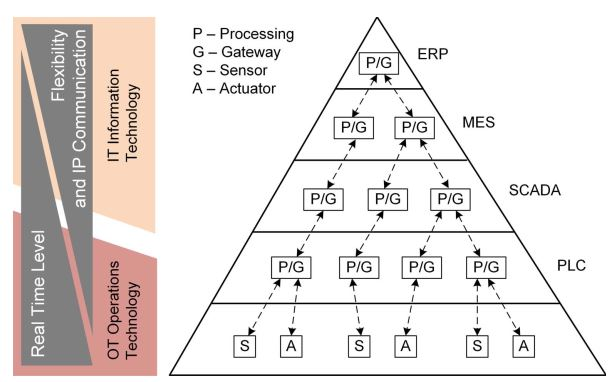
\includegraphics[width=0.7\textwidth]{imgs/intro-industryarchitecture2.jpg}
    \caption{Classical automation pyramid structure, source from \cite{tsn_intro}.}
    \label{fig:pyramid-classic}
\end{figure}

Coming from top-level-related frameworks, there is, e.g., the OPC UA project; whereas names like Profinet,
DeviceNET, EtherCAT, Powerlink, etc, come from the field bus side---the lowest level. All of them have developed in an individual way as response
to market needs, however meeting in the late decade through the necessity for unified standards to improve interoperability between the incredible number
of projects. This happens at a time were information, technical as well, and development tools have become even more available and
open to the end-user and the developer. Leading then now to a situation where the private initiatives are not any longer the full owners of the technology development.
See Fig.~\ref{fig:pyramid-iiot} for the IIoT's approach.

\begin{figure}[h]
    \centering
    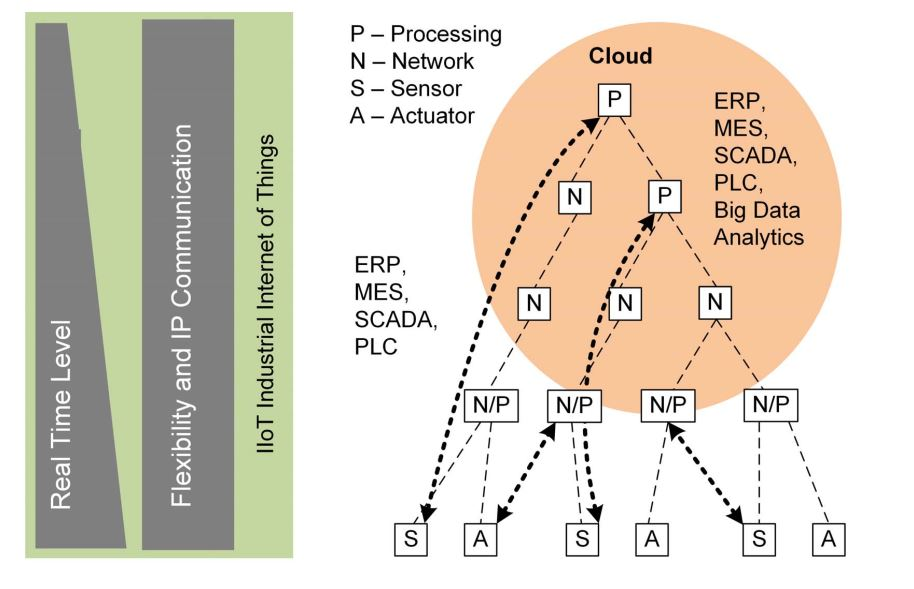
\includegraphics[width=0.7\textwidth]{imgs/intro-industryarchitecture.jpg}
    \caption{\emph{Industry 4.0} a more flexible automation structure. Industrial Internet of Things, source from \cite{tsn_intro}.}
    \label{fig:pyramid-iiot}
\end{figure}

Another line of work, closely related to interoperability, is the Real Time (RT) applications in their both versions with \emph{hard} and \emph{soft} requirements. 
Nowadays, there is an increasing number of applications in robotics that demand control loops and device chains that
require hard real time performance. Although these requirements are more common at the operational technology level, such as, robots, CNCs, servo motors, etc. 
They all face now the IIoT demands; hence, their networks should meet as well certain degree of RT capability. 
Moreover, synchronization of time sensitive
systems within manufacturing lines, for instance, has been addressed for years by the RTE protocols and now this kind of features are increasingly
been demanded as well at upper layers.

The current automation industry has many competitors and close technologies, as a natural consequence for specific processes requirements---depending on the industry;
but also as a response of the market. However, the search for standardization
can be tracked back to the 1980s, as the field buses were standardized by the International Electrotechnical Commission (IEC). 
This continued and Ethernet took its place within the industry. As an important note, during the last two years, according to the HMS Industrial Networks' annual study,
the total market shares of new industrial nodes in factory automation increased for the Industrial Ethernet from \num{52}$\%$ to \num{64}$\%$; while the
field buses decreased in the same period from $42\%$ to only $30\%$. Finally, the industrial wireless remained around the \num{6}$\%$, see Fig.\ref{fig:fieldbus_shares}.

It is yet worthy to mention that the name \emph{Industrial Ethernet} is used only as a 
generalization for the group of protocols that historically developed on IEEE's Ethernet specification; even though they all are almost no further
compatible with each other---because of the modified Media Access Control (MAC) layers. 
Details about the differences is addressed in the following chapters.  

\begin{figure}[h]
    \centering
    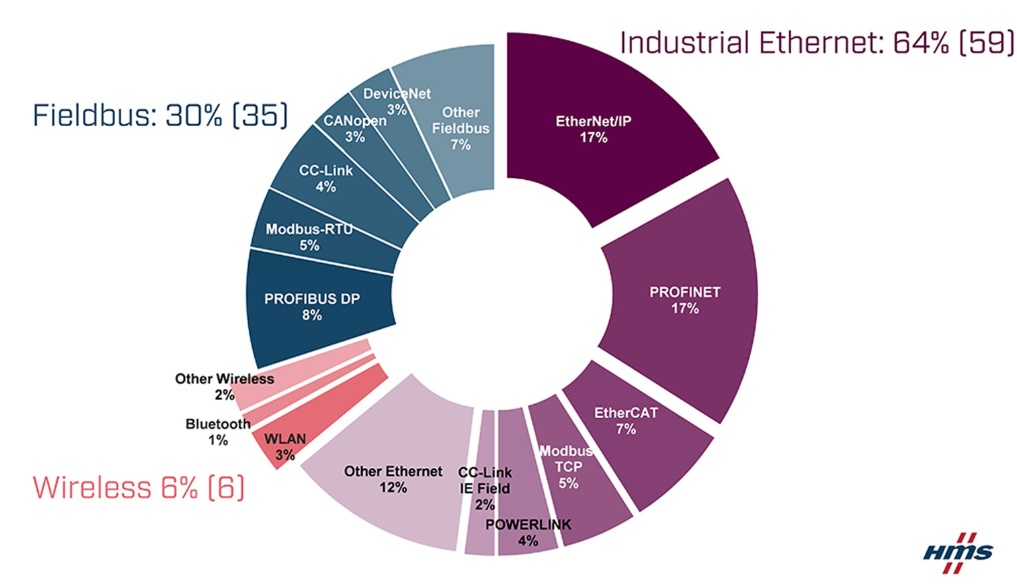
\includegraphics[width=.8\textwidth]{imgs/intro-buses-share.jpg}
    \caption{Industrial network market shares 2020 according to HMS Networks. Source from \cite{fieldbus_shares}.} %Add the reference, this could be a table
    \label{fig:fieldbus_shares}
\end{figure}

Vendor protected technology has its limit when there are plenty of possibilities for automation technologies, even if they are in ongoing development. 
For instance, as happened during the lifetime of the Open Platform Communications (OPC) project---predecessor of OPC UA---that was started only upon Microsoft Windows and 
as the time went by, the emerging needs made it change to use open standards and a multiplatform approach.

To introduce the reader to a common ground regarding standardization, the following section will present a brief summary of the standards that 
are of interest for anyone who wants to start developing using industrial interfaces.

\section{Industrial standards and the TSN initiative}\label{sec:standards} 

This section is intended to provide the starting developer a rough but useful reference of the standards related to industrial 
communication networks. 

First, due to the historical and technological process of innovation within the information and communication 
systems, several parties have been related and, at some extension have merged results, bringing out an interconnected 
set of norms that thrive continuously onto a global standardization.

The following list is intended to be a quick reference to the current standards for Ethernet, legacy and current field buses, 
Time-Sensitive Networks in their American and international initiatives. This way, the reader has a roadmap to be taken into
account for deeper research within the industrial applications. 
Furthermore, information related to the similar standardization processes between 
the IEC, ISO and IEEE, and their unavoidable cooperation, can be read in \cite{standards_coop}. %a comparisson of the ieee and iec standars processes

\begin{description}
    \item[ISO/IEC/IEEE 8802-3:2015] Revision of the Ethernet standard for half and full-duplex communication up to \SI{100}{\mega\bit\per\second}. 
    Originally published by American IEEE 802-3 in 1985 and accepted internationally in 1989. The last revision 8802-3-2017/Amd 10-2019 includes
        MAC controls for \SIlist{200;400}{\giga\bit\per\second}. More information in \cite{iso8802_ethernet}. %https://www.iso.org/standard/72048.html 
        After 2019 The name Ethernet is not longer used, instead CSMA/CD or a reference to the corresponding ISO standard 8802.3 is the formal name.
    \item[IEC 61158:1999-2000] First international field bus standard published in 1999, where 8 \emph{Types} of field buses were introduced addressing the 
        Physical Layer (PhL), the services and protocols of Data Link Layer (DLL) and Application Layer (AL). Some included brand 
        names were the following: H1/HSE/H2, ControlNet, EtherNET/IP, Profibus, Profinet, Interbus. This standard has an interesting story
        concluding with the signing of the \emph{Memorandum of Understanding} by the main contenders to put end to the field bus war. The latter can be reviewed in \cite{fieldbus_history}.%The Fieldbus Standards: History and Structures
         The standard's most updated version in 2019 includes 26 Types of protocols, creating out of them the so-called Communication Profiles (CP), likewise grouped
        into field bus Communication Profile Families (CPF). 
    \item[IEC 61784-Part 2:2008] It is extension for the RT capable CPs that are based on the IEEE 8802-3 standard. Commercial names included 
        are the next: EtherCAT, Profinet, Ethernet/IP, Ethernet Powerlink, and Modbus TCP. An interesting overview of the current development 
        of the industrial communication networks can be reviewed in \cite{future_iiot}. %Industrial Communication Systems and Their Future Challenges: Next-Generation Ethernet, IIoT, and 5G
        The SERCOS CPF is highlighted, since its third version is, altogether with the EtherCAT profile, the fastest one in the list; providing as well
        a more efficient use of the available bandwidth with an open source resources. It shows even advantages over CAN devices due
        to its original design intended for hard RT motion control; for more information review \cite{sercos_origin} and \cite{sercos_performance}. %https://www.designnews.com/sercos-picks-pace %https://www.sercos.org/technology/advantages-of-sercos/performance/. 
        This is a very interesting hard RT protocol whose applications might need further study out of the scope of this 
        Research Project.
    \item[IEEE 802.1A/B/C/D/Q] Time-Sensitive Networking standards is an initiative to improve the IEEE 802-3 in order to meet the industrial real time requirements, 
        which story can be tracked back to 2005, as the IEEE 802-3 group was merged with the IEEE 802.1 Audio Video Bridging Task Group and started to work for
        industrial environments. This a response to the vast alternatives of the RTE CPs. About 60 individual IEEE standards oriented to improve
        the ISO/OSI layer 2, including 13 focused on its security, are within the scope of the TSN project. A nice introduction to this standard's scope can be read from TSN 
        section in \cite{future_iiot}. %section about the TSN
        The mentioned project covers the lower layers of the communication system, whereas the upper ones, representation and transfer of data, is
        addressed by OPC UA. Moreover, it is important to mention that this is an ongoing project and still around $40\%$ of its standards are
        in draft or preparation phase. For further information regarding the current standard development, visit \cite{tsn_homepage}.
    \item[IEC/IEEE 60802] TSN Profile for Industrial Automation is the stand alone TSN base standard that will include the common advancements
        from IEC SC65C/WG18 and IEEE 802 work groups mentioned in the previous item. See \cite{tsn_profile} for the current development group's activities. %https://1.ieee802.org/tsn/iec-ieee-60802/
        This is an ongoing project started around 2017, still being in a draft phase. Since this will be the international standard, it would be 
        the equivalent to the effort once given during the creation of the IEC 61158 for the legacy field buses.
    \item[IEC 62541:2016-2020] Set of IEC standards for OPC UA. Individually, the IEC 62541-14:2020 defines the OPC Unified Architecture 
        (OPC UA) PubSub communication model. It defines an OPC UA publish/subscribe pattern which complements the client server pattern defined 
        by the Services in IEC 62541-4. IEC TR 62541-1 gives an overview of the two models and their distinct uses. For the concrete list of contents, review \cite{opcua_standard}. %https://webstore.iec.ch/publication/61108  
        An overview of this technology and how it is planned to complement the TSN can be reviewed in \cite{opc_tsn_application}. %Open Source OPC UA PubSub over TSN for Realtime Industrial Communication
\end{description}



% CANopen protocol is not capable of hard real time capabilities?


% >>Here comes information about SERCOS. The SERCOS interface started as a project for providing a Hard Real Time capable communication
% bus, it has been developed during the years, having nowadays three versions. The first ones operating over a serial bus and submitted
% to the IEC, which in 1995 released it as IEC 61491.[2] After the release of the original standard, original working group member companies 
% including ABB, AEG, AMK, Robert Bosch, Indramat, and Siemens founded the "Interest Group Sercos" to steward the standard. \ref{dummy} %https://en.wikipedia.org/wiki/SERCOS_interface#cite_note-3
% Even though the capabilities meet hard real time requirments, compared to other technologies, is rather limited. %https://en.wikipedia.org/wiki/SERCOS_interface#cite_note-3
% For the last version it has been capable to address up to 60 Motion Axes and makes use of the Ethernet standard, making it an alternative
% for the mentioned technology comming from BEckhoff. Together with EtherCAT, Sercos is the fastest 100Mps industrial Ethernet technology.
% One advantage so far of this protocol is its parallel development with the OPC UA, making it natively compatible with such networks* 
% and security layers.



\chapter{State of the art}\label{cha:state}

%% Proposed roadmap
%
%   The use of RT in the industrial environments
%   Current standards IEEE and IEC and the TSN
%           Roadmap of standards
%           RTE protocols and OPC UA   
%           How are they related
%  
%   -----------State of the art--------------------------------
%   Applications with RTE and OPC UA in Hard Real Time applications     
%   A brief overview about the RT tools in robotics
%           The importance of EtherCAT as an open RTE protocol within robotics
%   Comparison of openess
%   EtherCAT introduction (selected by Hans Robot)
%           Focus on EtherCAT XoE <<THIS ONLY NEEDS TO BE MENTIONED
%------------------Out of scope--------------------------------------
%   HW ASICS and stuff like that
%   SW Stacks for EtherCAT development and other RTEs
%

This chapter introduces some current applications mainly focused on robotics, since this area is closely
related to the environment with which the ACB will be interacting. Robotics sees various advantages
from the RT communication protocols, when it comes to integrate motion controllers and 
any other industrial peripheral. Afterwards, an overview about industrial development frameworks is 
given, yet focused not on the RT interfaces, but its specific software. The latter is of great importance,
for the Real Time Operative Systems (RTOS) are a corner stone for embedded systems that need to provide a 
deterministic service within their environment.


\section{Current applications}\label{sec:applications}

As rapidly mentioned in Sect.~\ref{sec:standards}, the SERCOS motion control interface has been standardized within the 
CPFs of IEC 61784-Part 2. Furthermore, it has been even integrated to EtherCAT as a compatible CP. 
This service is available within the DLL and AL and is called Servo Drive Profile over EtherCAT  (SoE), 
which provides access to motion controllers under 
the SERCOS specifications and, consequently, offers interoperability within its own RT features and the latter's hard RT 
capabilities.  
An example of this compatibility is presented in ~\cite{ecat_sercos}, %Motion Control System using SERCOS over EtherCAT
it shows that jitter of 30 microseconds is feasible in a control loop while the Master uses the SoE service.

Another interesting application has been the characterization of an EtherCAT Master within a RT control 
loop for Servo Motors, which run CAN devices over EtherCAT (CoE service). The implementation of the Master 
device ran on different open source Real Time Operating Systems (RTOS) based on Linux, 
namely, Xenomai and Linux with the \emph{RT\_PREEMPT} patch. It was concluded that both of the approaches 
were capable to achieve update periods of \SI{1}{\milli\second} 
, and an average jitter of \SI{1.5}{\micro\second}. Moreover, Xenomai could averagely achieve execution times around \SI{100}{\micro\second}; 
the mentioned data can be reviewed in ~\cite{ecat_xenomai}.%Real-time Servo Control using EtherCAT Master on Real-time Embedded Linux Extensions. 
It is worth to mention that the EtherCAT Master features were available in both RTOS kernels, 
for the IgH EtherCAT Master stack was running on top of them. This open source stack will be commented in ~\ref{sec:openness}.

The characterization and optimization of performance for different RTE profiles within TSN is a currently expanding topic, 
as the TSN standards and the RTE commissions are still working together. In ~\cite{tsn_and_sdn} %Integrated Industrial Ethernet Networks: Time-sensitive Networking over SDN Infrastructure for mixed Applications
are presented simulations of TSN topologies with EtherCAT and SERCOS data frames, where the Quality of Service (QoS) 
is addressed and evaluated through the usage of Software-defined Network (SDN) switches. 
The approach of this project is to test different scheduling features given fixed cycle times for the data frames, 
which were proposed to be similar to the current real industrial applications
in both technologies. In this manner, the importance of an unified network that supports different protocols is highlighted, 
but further research in this topic, including tests with other RTE data frames are still to be researched.

Besides robotics, a recent industrial application concerning CBD extraction equipment for high-performance large-scale processing,
implemented distributed control and monitoring based on EtherCAT open protocol. This article can be seen in ~\cite{ecat_industrial}.

Addressing the usage of open source tools, such as OS and RTE Protocols, for development of complex robotic systems, in ~\cite{ecat_motionplanning} %Motion Planning for Quadrupedal Locomotion: Coupled Planning, Terrain Mapping and Whole-Body Control
is presented a \emph{Motion Planning for Quadrupedal Locomotion}. This is roughly composed, besides the hydraulic actuators, mechanics and other peripherals, of two PCs on board with RT capabilities and shared memory. 
RT Linux (Xenomai) runs on both of them and take care of different levels of the control threads at two different rates depending on the tasks, 
namely \SI{1}{\kilo\hertz} and \SI{250}{\kilo\hertz}. The former rate is used
for communicating with the motor controllers over EtherCAT interfaces.

Currently, Han's Robot Germany GmbH focuses on enhancing robots’ cognitive abilities by developing in the fields of environment perception, 
drive technologies, 
control theory, material science, mechanical design and artificial intelligence. Interfaces within the robotic system rely on various
industrial protocols to make its interoperability one of the key features. For instance, current motor drivers
are linked over internal EtherCAT chain to the main controller.

The above mentioned applications are just a tiny number of examples that shows the importance of an already standardized open industrial communication protocol, 
within a broad set of fields that cannot be completely covered in the scope of this document. Nevertheless, it paves the road to understand why generating the know-how 
to any of the mentioned technologies, represents a high-impact resource for any research or development group, regardless of its commercial or academic purposes.

\section{An overview about the RT capable SW in robotics}

As mentioned in the previous section, several resources and examples showed the current usage of RT
open source software and its community. Since this Research Project has a goal of introducing the reader a 
roadmap for RTE communication interfaces and 
its applications, this section was added to summarize the RT software for development in robotics.

The usage of middlewares within the field of robotics is growing and it relies on \emph{robot software} that 
exists between the application and an RTOS, as detailed in the following articles ~\cite{ecat_xenomai} and ~\cite{ecat_motionplanning}.%the robot examples.

A list of requirements is suggested in ~\cite{middleware_industrial} %2020-Real-Time Robot Software Platform for Industrial Application 
to address the mentioned middlewares and how to consider them \emph{Real Time Robot Software Platforms}.  
The list is as follows and it is useful to start getting familiar with the capabilities 
and features of the so-called Robot Software: 
\begin{enumerate}
    \item Data exchange support.
    \item Real time support (strict periodic execution and sporadic events support).
    \item Thread and process types for user defined programs support.
    \item Easy configuration of applications (robot control SW, PLC SW, vision inspection SW, non-real-time SW, etc.)
    \item Multiple periods for scheduling.
    \item Threads or processes running in the same period are classified by priority.
    \item Check and handle the event through the event handler.
\end{enumerate}

Common names for different projects aiming to create these development frameworks are the following: Common Object Request Broker Architecture
(CORBA), Real-Time CORBA (RT-CORBA), Data Distribution Service (DDS), OPC UA, Open Platform for Robotic Services (OPRoS), 
Open Robotics Technology Middleware (OpenRTM), Open Robot Control Software (OROCOS), 
and Real-Time Middleware for Industrial Automation devices (RTMIA). Further comments and a comparisson between their features
can be seen in the previously referenced paper. As to what concerns to this document, only some of them will be roughly commented
as they ended up being somehow related to the RTE profiles. For more information review ~\cite{middleware_xbotcore}.

\begin{description}
    \item[OPC UA] As frequently mentioned before, this is an open standard for data sharing among nodes within industrial networks and has
    been considered in some projects related to robotics. Nevertheless, it is important to highlight that this is not considered a full 
    middleware, since it only provides a protocol to control the exchange of data between nodes, a good degree of reliability and security.
    However, it does not provide RT capabilities to the system only compatibility. Hence, it needs an operative system and the consequent 
    lower layers capable of RT scheduling and communication, concerning the latter the TSN set for protocols is an example.
    \item[ROS/OROCOS/OpenRTM] These are projects that aim to create a suitable middleware for robots by implementing Xenomai or Linux operating systems. 
    ROS prioritizes the final user, avoiding in the way some fine-grained features due to its difficulty, therefore having sometimes
    issues to meet the hard RT requirements. Whereas OROCOS has further improved its compatibility, similarly to OpenRTM.
    \item[CODESYS and TwinCAT] To fully meet compatibility with the industry, the so-called PLC Software has been also used in open robotics.
    These applications essentially need to run both, the robot functional blocks and the robot tasks. For further details on it the following
    references can be reviewed ~\cite{middleware_xbotcore} and ~\cite{middleware_xbotcloud}. %referemces from the italian robot Xrobotcore
    \item[xbotcore] This is an attempt to provide of a highly compatible open middleware for industrial robotics, it runs over the Xenomai and 
    uses a SOEM stack to interface with any compatible industrial device, recall ~\ref{sec:openness}. % XBotCore: A Real-Time Cross-Robot Software Platform 
    Applications have been already mentioned in ~\ref{sec:applications}, which have reached control loops down to 1khz for 33 axes. More details about the 
    latter application in ~\cite{middleware_xbotcore}.
    %\item[RTMIA] RTMIA middleware + Linux or Xenomai but used open PLC running parallely[?] << This needs further reading [?]
\end{description}


The previous information was presented only to draw an idea for the non-familiar reader about the applications and, since this topic is in ongoing development 
and, furthermore, many other platforms are addressing similar challenges; the reader is invited
to go deeper into these topics, for instance, by reviewing this resource ~\cite{middleware_industrial}. %add the resouce fromt he open community 

\section{Approaching openness within the RT protocols}\label{sec:openness}

Among the industrial standards mentioned in ~\ref{sec:standards}, there are some related initiatives to include a certain degree of open source
software to improve the development of applications. The following is a brief list of a few interesting references to them. 
However, as expected, most of the software stacks
for industrial communication systems are commercial and provided by third-party companies. 

%90/100
\begin{description}
    \item[OSADL] Open Source Automation Development Lab eG (OSADL):It is a German group that intends to lead the development of open source development
    for industrial automation. Closely related in the developing of OPC UA and other Linux features for industrial applications.
    \item[open62541] Within the official scope of OPC UA, there is this Certified SDK project that is within its second phase, at which it is expected 
    from the research and industrial community to develop applications to test its performance. Moreover, as the TSN specification is of huge importance, 
    a set of enhancements for the open62541 project were developed by Fraunhofer IOSB and series of patches for the Linux kernel have been released to 
    make it an RT compatible. To review the overview of the project, visit ~\cite{open62541_homepage}. %https://www.osadl.org/OPC-UA-over-TSN.opcua-tsn.0.html 
    The OPC UA is developed under GPL 2.0 license and due to its current phase implies a further adaptation for the physical node, e.g., ARM arquitechtures 
    to make them compatible with the mentioned patches. 
    \item[SOEM/SOES] RT Labs Industrial development group focused on Software Stacks for industrial protocols. Among their commercial communication stacks
    there are software stacks under GPL for EtherCAT Master and Slave devices SOEM/SOES. More details about these stacks can be found in ~\cite{soesm_homepage}. %https://rt-labs.com/product/soes-ethercat-slave-stack/ 
    \item[Sercos Stacks] Sercos III technology is able to be operated in a common TSN-based network, % Ethernet TSN heralds a new era of industrial communication
    since its development group has been working closing together with the TSN group; a more detailed scope can be seen in ~\cite{sercos_tsn}. 
    They also made available open source software dedicated for development of master and slave devices, namely: Common Sercos Master API (CoSeMa),
    Sercos Internet Protocol Services (IPSS), and The Sercos III SoftMaster, the latter even allows the host to use any standard Ethernet controller. %https://www.sercos.org/technology/implementation/driver-software/. 
    It is important to mention that there are testing tools to certificate those devices and achieve a Safety Integrity Level 3 (SIL-3). A description of the
    different available libraries is provided in ~\cite{sercos_stacks}.
    \item[EtherNet/IP Stacks] There are several commercial stacks that comply with the Open DeviceNet Vendors Association's (ODVA) EtherNet/IP specification. 
    OpEner is an open source alternative which targets PCs with a POSIX operating system and a network interface. 
    Integration examples are provided only in Linux and Windows in ~\cite{opener_stack}; %http://eipstackgroup.github.io/OpENer/index.html
    nevertheless, a variation for embedded systems has been presented for an STM32 microcontroller. In the mentioned project, more tools had to be adapted, for instance,
    STM32F4x7 Ethernet Driver v1.1.0, lwIP v1.4.1 (TCP/IP Stack), MicroHTTP v5.1.0.1, a patched version of OpENer v1.2., among others. A detailed description
    of the requirements can be reviewed in ~\cite{opener_stm32}%https://www.emb4fun.de/archive/chibiosopener/index.html
    \item[IgH EtherCAT Master] This is a bundle of libraries to give a Linux host (LinuxCNC for example) EtherCAT Master features, it is developed under the GPLv2 license. 
    An interesting example of this open source resource within an Airbus Test Rig can be reviewed in the following reference ~\cite{ecatstack_igh}. %https://etherlab.org/en/success/airbus-testrig.php
\end{description}

As the scope of this Research Project is only focused on the industrial communication profiles capable of RT and, so far has been clear how 
the EtherCAT is a reliable one, yet open and significantly considered in the industry ---recall Sect. ~\ref{sec:applications}. 
Hence, it makes sense to invite the reader to read the introduction to the protocol itself in the Appendix ~\ref{sec:ecat_protocol}. 
This way it is easier to go sensibly to the implementation of what is one of the basic chain-elements in what could become a very complex application: 
an EtherCAT Slave device with open source elements.


\chapter{Design requirements and approach}\label{cha:solution}

This chapter presents the main goals of the project and the technical specifications. It is also 
intended to give the reader a summary of the proposed functional modules and its structure. 
Any other constraint not mentioned here 
was adjusted or set while being within the design-test loop, as consequence of the prototype nature of the project.
\section{Objectives}
The main goal of this project is to develop a device using open-source tools to read out sensor data from a robot
axis that can be interfaced with an RTE Network. Such that this device can be used afterwards as a test platform 
within an industrial environment to characterize its compatibility with the ongoing IEC/IEEE 60802
TSN Profile for Industrial Automation.

To achieve the main goal the following has to be carried out:
\begin{itemize}
  \item To specify the requirements of the system
  \item Comparison considering the state of the art
  \item To develop the embedded system as a functional EtherCAT Slave Device
  \item To design and manufacture a PCB prototype
  \item To test and report the overall system functionality
\end{itemize}

\section{Technical specifications}

In the table \ref{tbl:tech_specs} the requirements for this project and their state after the implementation can be observed.
This comparison helps as a good summary of the overall achievements that are further detailed in the next chapters.

  \begin{tuhhtable}
    \footnotesize\centering
    \begin{tabular}[hbp]{L{.22\textwidth}L{.22\textwidth}L{.22\textwidth}L{.22\textwidth}}
        \THc{1}{c}{Feature} & \THc{1}{c}{Requirement} & \THc{1}{c}{Implementation} & \THc{1}{c}{Remark} \\
      \abovebodyrule
      \TRh{1}{l}{Upper layer interface}  & Ethernet/EtherCAT compatibility.\newline Non-safety relevant.\newline Services and synchronization: - 
                                        & EtherCAT slave.\newline Services: Mailboxing and CoE\newline Synchronization: Free Run and SM  
                                        & \tblYes\newline FoE and SD synchronization possible in the medium term.\\\TRc
      \TRhc{1}{l}{Display/signaling}    & LED stripes with serial interface:\newline WS2812 \newline 2 Ch  
                                        & 2-4 Ch modifiable in SW\newline Animation capable 
                                        & \tblYes\newline Chs can increase up to number of DMA-Timers (8)   \\
      \TRh{1}{l}{Temperature}           & Data interface for 1-Wire bus     
                                        & 1-Wire Master\newline 15 sensor in bus & \tblYes\newline 6 Sensors simultaneously tested \\\TRc
      \TRhc{1}{l}{PCB}                  & PCB Prototype\newline Layout and size: -   
                                        & Attachable PCB for LAN9252-EVB-SPI.\newline Size: \SI{55 x 38}{\milli\metre} & \tblYes\newline Second layout with both chips included possible in the short term. \\
      \TRh{1}{l}{Safety}                & \tblNA     
                                        & Non Safety-Critical for this prototype & \tblNo\newline FSoE could be researched in the long term.\\\TRc
      \TRhc{1}{l}{Extra interface}      & SPI or I2C interface for current/IMU/black channel   
                                        & Extra SPI considered in PCB and SW\newline JTAG/SWD compatible interface & \tblYes\newline Currently working \\
      \TRh{1}{l}{Speed/position}        & Possible interface of BISS-C type
                                        & Not required for this prototype & \tblNo \\\TRc
      \TRhc{1}{l}{Refresh data cycle}   & -   
                                        & No hard RT deadlines.\newline Deterministic refresh cycle of $\sim$\SI{10}{\milli\second} by RTOS.\newline Timeout faults handling. & \tblGood\newline Timing through RTOS  \\
      \TRh{1}{l}{Data structure}        & -     
                                        & Functional and parametrization data structure as Object Dictionary.\newline Standard ESI file. & \tblYes\newline Currently working\\\TRc
      \TRhc{1}{l}{FW programming}       & -   
                                        & CMSIS - FreeRTOS for thread, event and time management. & \tblGood\newline Currently working \\
      \belowbodyrule
    \end{tabular}
    \caption{Technical specifications;}
    \label{tbl:tech_specs}
  \end{tuhhtable}

Regarding the functional safety features of the device, it is important to mention that, even though this device is considered as non Safety-Critical within
this prototyping stage, the means to create a framework that could be extended to address further reliable development are taken into account, namely
by considering fault tolerance within the software. More comments about this will be done in the results section. 

\section{Solution proposal}
In Fig.~\ref{fig:sysStruct} the proposed layered structure of the functional blocks can be seen, this will help the reader
localize how is the level of interaction of each of the parts that are described along the document. For instance, the project itself 
focuses mainly on the non-dashed blocks; nonetheless, they still need to be configured or adapted according to ACB features. The layered
representation shows three general concepts, namely physical or hardware, middleware and application software. Even though, the blocks
help the reader differentiate between functionalities, most of them are interacting between each other, mostly the Devices' State Machines (DSM).

\begin{figure}[ht]
  \centering
  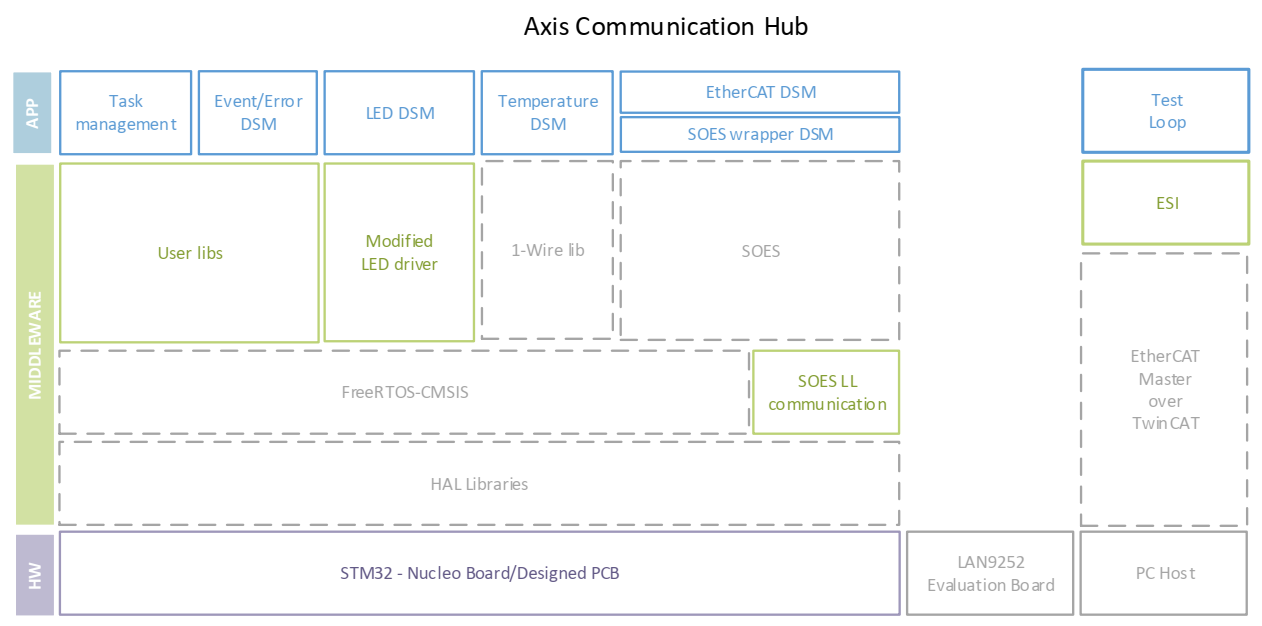
\includegraphics[width=\textwidth]{imgs/prop-system_struct_v2.png}
  \caption{Layered structure of the proposed functional blocks.}
  \label{fig:sysStruct}
\end{figure}

\section{Hardware selection}

In this part it is presented the base hardware that was available to develop the prototype. The microcontroller (MCU) was chosen
due to its active community, resources and current on-develop projects. Other MCUs were though considered, since the overall characteristics
were somewhat similar and generic---regarding peripherals like serial interfaces or Direct Memory Access (DMA) and processing power and memory, for instance.
Therefore, MCUs from Infineon and 
Texas Instruments were good possible candidates---see technical information in ~\cite{infineon_esc},~\cite{infineon_dramfine} and ~\cite{texasi_esc}, respectively; 
however, the basic familiarity with the STM32CubeIDE and the related ST technology 
was a crucial factor. In addition, and concerning the chosen MCU as well, the learning curve is not negligible when it comes to develop any 
firmware at a fair level, even more when it deals with other to-learn
tasks, for instance, development with RTOS, modification of open libraries, EtherCAT protocol itself and the Network Controller chip.

Regarding the Network Controller, the LAN9252 belongs to a set of ASICs that are verified and certified by Beckhoff Automation GmbH. For a further
reference for other alternatives visit ~\cite{beckhoff_esccomparison}. The LAN9252 integrates a so-called EtherCAT Slave Controller (ESC) and it represents a good 
alternative to the Beckhoff's original ASIC ET1100. This way, the basic hardware is there to fulfill Han's Robot Germany's
proposal for developing industrial compatible devices that could enhance the prototyping process within the electronics department. 
Moreover, the mentioned ASIC has a wide compatible control interface that make it be suitable to any microcontroller with which 
the developer has experience. The Table~\ref{tbl:hardware_characteristics} lists the main characteristics of the above mentioned hardware.

\begin{tuhhtable}
    \footnotesize\centering
    \begin{tabular}[tp]{L{.44\textwidth}L{.44\textwidth}}
        \THc{1}{c}{STM32F446ZE} & \THc{1}{c}{LAN9252} \\
      \abovebodyrule
        ARM®32-bit Cortex®-M4 + FPU + Chrom-ART™ Accelerator
        Up to 180MHz CPU\newline
        512 kB of Flash\newline
        128 KB of SRAM
                                        & EtherCAT slave controller with
                                        3 FMMUs and 4 SyncManagers\newline
                                        Distributed clock support\newline
                                        4KB of DPRAM\\\TRc
        General-purpose DMA\newline
        Up to 17 timers\newline
        Up to 4 × I2 C interfaces\newline
        Up to 4 USARTs/2 UARTs\newline
        Up to 4 SPIs\newline
        2 × CAN (2.0B Active)\newline
        USB 2.0 full-speed device/host/OTG 
                                        &100Mbps Ethernet transceivers compliant with IEEE 802.3/802.3u (Fast Ethernet)\newline
                                        8/16-Bit Host Bus Interface, indexed register or multiplexed bus\newline
                                        SPI/Quad SPI\newline
                                        Digital I/O Mode\newline
                                        Multifunction GPIOs
                                        \\
        LQFP64, LQFP100 and LQFP144 packaging     
                                        & Pb-free RoHS compliant 64-pin QFN or 64-pin TQFPEP packaging 
                                        \\\TRc
      \belowbodyrule
    \end{tabular}
    \caption{Summary of the characteristics of both STM32F446ZE and LAN9252 used in the prototype.}
    \label{tbl:hardware_characteristics}
  \end{tuhhtable}

%\subfigbox{
%    \subfigure[NUCLEO-STM32F446ZE]{\label{subfig:stmboard}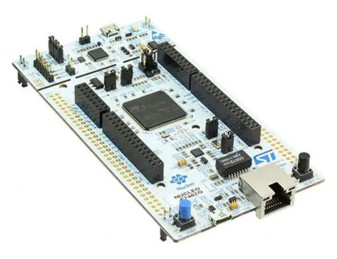
\includegraphics{imgs/sol-stmboard.jpg}}
%    \subfigure[LAN9252-EVB-SPI]{\label{subfig:lanboard}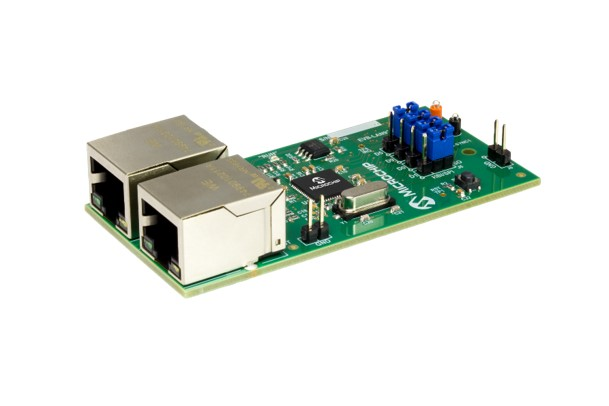
\includegraphics{imgs/sol-lanboard.jpg}}
%}{Evaluation boards for prototyping.}{fig:evalboards}

\begin{figure}[ht]
    \centering
    \subfigure[NUCLEO-STM32F446ZE]{\label{subfig:stmboard}{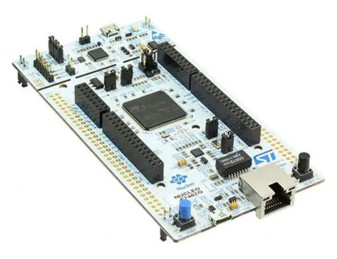
\includegraphics[width=0.4\textwidth]{imgs/sol-stmboard.jpg}}}\hfill
    \subfigure[LAN9252-EVB-SPI]{\label{subfig:lanboard}{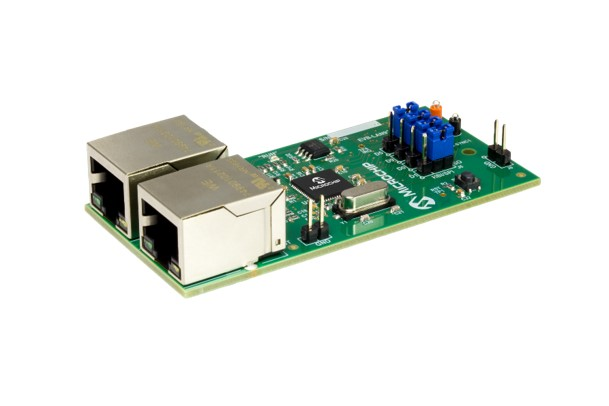
\includegraphics[width=0.4\textwidth]{imgs/sol-lanboard.jpg}}}
    \caption{Evaluation boards for prototyping.}
    \label{fig:evalboards}
\end{figure}

\section{PCB design}\label{sec:pcb_proposal}
As it can be seen in the figure \ref{subfig:lanboard}, the evaluation board includes on-board male pins, this was taken as an advantage and the PCB to be designed
consisted on a pluggable PCB that would be mounted on top of it, increasing minimally the volume already occupied by the evaluation board. This idea needed to be 
designed taking into account the minimum of components based on the Nucleo-STM32F446ZE original design and the requirements of the LAN9252. This means that 
it had to provide, both 5V and 3.3 V power supply, physical ports for the prioritized communication capabilities, minimally SPI, One-Wire JTAG and the LED ports 
according to the technical specifications \ref{tbl:tech_specs}.

\section{Firmware structure}

Since the compatibility with the EtherCAT protocol is the highest priority, all the tasks related to the adjustment of existing libraries and 
the synchronization between them are also prioritized, such that the main functionality can operate. Taking this into consideration and 
recalling the final proposal for the structure of the embedded system, Fig.~\ref{fig:sysStruct}, the functional blocks are represented differently. 
The ones in gray or dashed lines are mainly components that are planned not to be modified
at all or not in deep, because of either its complexity or its given reliability. This means, its functionality is almost granted. 
Nevertheless, the progress relies on documentation that can be either good or poor, for instance, TwinCAT has good resources, 
whereas SOES does not. Regarding the latter, the block refers to the main library to be integrated, that enables the EtherCAT features; 
although, 
it is represented with dashed-lines, it was changed but not restructured.
However, detailed information about these concerns are presented along the implementation and result chapters.

The word firmware rather generalizes the set of written/modified code that needs to be carried out through the implementation, for instance, the
top layer in blue corresponds to the application-related source files written in C, while the Test loop executes over TwinCAT3 and is written
in SText, which needs mandatory an EtherCAT Slave Information (ESI) file written in XML. The name middleware, in this case, represents not 
only the Hardware Abstraction Layer (HAL) libraries provided by STM, nor the CMSIS-RTOS's, but also represents the user-define libraries for each
DSM and the modified libraries, namely those for the LED and One-Wire---as well as the already mentioned case of SOES. This structure is important to have
in mind, mainly while going through the implementation chapter.

Additionally, another thing to consider within this document is the abbreviation \emph{DSM} (Device's State Machine) which is used as substitute for State Machine,
such that it is not confused with Synchronization Manager, defined as well by Beckhoff Automation as SM.



%TODO this figure needs to be updated changing the Error handler to Event handler, configuration/management to auxiliar functions --monitor for debugging
%adding as well the ESI file as a functional block running on top of the LAN9252 Evaluation board
%Where could I mention about the wrappers used to integrate the functions contained within the 3rd party libraries and my SMS?
\chapter{Implementation}\label{cha:implementation}
The following chapter documents the different functional modules that were implemented according to the proposal. 
The tasks related to EtherCAT compatibility and usage of RTOS are highlighted within this and the following chapter,
 as they were of higher priority.

Moreover, the functional blocks or modules interact with each other through the DSMs, which has been added as well 
as a module for its understanding.

\section{LED Control}\label{sec:leds}


In order to notify to the user the current state of each axis, the robot includes one or more LED rings. These rings are 
 a serial array of LEDs that are programmed and controlled through a serial communication protocol. Basically, the final implementation
 is an adaptation of a library that uses a PWM peripheral to generate a signal that is modulated according to the data that 
 controls the LEDs, namely digital 1s, 0s and reset as a specific duty cycle. The input pin of the first LED is connected to the MCU and depending on the modulated data, it will be 
 passed over the next LEDs, being the first LED's output the input of the next til the last component. A summary of the 
 protocol is explained in ~\cite{led_protocol}. 

Furthermore, the current LED control in the robotic system uses MCU Devices without communication capabilities leading to 
static status indication that cannot be set from the Master.

 In the next paragraphs a summary of the activities that were carried out during the implementation is presented.

\begin{description}
\item[First control tests] Learning the basics of the interface used to control one LED
\item[Code for one LED control] Using the peripherals of the MCU simple routines were written to set different basic colors in RGB. 
    The peripheral used were a two Timers (hardware libraries) to keep control of the data timing and refresh rate.
\item[Search for libraries] Once the basic communication was understood, it was clear that the usage of libraries would be more practical,
    since the first approach were not suitable for higher number of LEDs and effects; moreover, the CPU was kept busy while waiting 
    the timer state polling. The libraries found were aiming roughly either 8/16 bits processors whose main task was controlling the LEDs, 
    or more complex libraries that used DMA modules within 32-bit processor. One of the latter implemented modulation of the data over a PWM and a
    DMA peripheral for one LED strip.
\item[First library selection] Due to the inexperience working with DMA modules and as the LED control was not of a higher priority compared to other tasks, 
    it was decided to run first one of the basic libraries to achieve a multi LED control. The implementation was able to control a set of 20 LEDs
    with the processor mainly polling the Timer states.
\item[Further control tests] Despite the success of the library with one channel, the overall structure of the basic library
    was not easily portable to the proposed solution using FreeRTOS. Additionally, the DMA libraries showed afterwards being easier 
    to modify as they were designed with a more abstracted and multi-purpose approach.
\item[Second library selection] As the usage of DMA became clearer, it was decided to improve the approach by 
selecting a 32-bit processor based library, that implemented only general control functions to avoid massive code lines
related to effects and other rather unnecessary features, yet structured enough to be easily adapted. 
The final result was based upon the WS2812 Library for STM32F4 from Uwe Becker, see \cite{led_library}. 
Main modifications were the addition of multiple channels capability and global flags needed for synchronizing with DSMs.
\end{description}


\section{Temperature acquisition}\label{sec:temperature}

Similar to the LED control's library, the temperature readout needed a library to be modified to match the current project.
\begin{description}
\item[First readouts] Working with the temperature sensors was the first task in schedule, so it helped train the basic usage
    of the IDE STM32Cube, along with the hardware configuration of the MCU and the HAL libraries. 
    The sensor uses a one-wire serial protocol, which similarly to LED Control's first approach was implemented by using 
    timers for controlling 1s and 0s high levels, a continuous polling of data and a general while loop approach. 
    This method worked as intended but it was known from the beginning that it would not match the multi-tasking proposal. 
    However, it was of great importance to get to know the hardware and software, besides more functions were needed to 
    access the sensor's ROM needed e.g. for identification.
\item[FreeRTOS first tests] Short after the working code was used to do the first tests with the RTOS, 
    in this manner the code was translated as a Task (Thread as called by CMSIS) and some features like prioritization, 
    task attributes, task handling and signals were tested with other generic functions, e.g. clocks and PWM generators. 
    However, this implementation was not able to handle multiple one-wire devices due to its absence of CRC comparison.
\item[Integration of library] Finally, it was decided to adapt one open source library designed for STM32 processors. 
    This is based on the principle that UART speeds at \SIlist{9600;11200}{\bit\per\second} suit the One-Wire timing, such that the 
    detection of One-Wire devices and communication process can be downloaded to hardware already included in many 
    general-purposes processors using USART. The integration of this library is from design compatible with RTOS, 
    namely with CMSIS-RTOS. The library selected was developed by Tilen MAJERLE, review in \cite{temp_library}, and it 
    was barely modified as it contained already the desired functionalities and the development
    focused only on the integration into the DSMs and usage of it. 
\end{description}

The strategy the final library is based on is rather interesting and more details can be read in \cite{onewire_theory}.

\section{EtherCAT Slave communication: SOES adaptation}\label{sec:soes}

This functional module had the highest priority, therefore most of the effort given was focused not only 
on the library itself but the protocol and the hardware commissioning, it is hence recommendable to read through the introduction 
to the protocol in Appendix~\ref{sec:ecat_protocol}. In this sense, the current section was structure
as follows: first, a bit more technical details are presented regarding the EtherCAT specification, and some constraints for 
the prototype such that the library could be tested accordingly to the scope of the project; afterwards the EtherCAT Slave
Controller (ESC) is briefly summarized and finally, the main points of the implementation are presented.

\subsection{EtherCAT data consistency and constraints for design}\label{sec:ecat_sms}
This subsection describes both the features with which the \emph{Axis Communication Board} has compatibility, and a summary of the mechanism that the protocol
implements at the low level to work with the data exchange between Master and Slave. The constraints that were set were part of a live process that ran 
all along
the learning process of the protocol. This is important to mention, since the understanding of the protocol leads to a sinful selection of the features
that a device should have implemented. Therefore, the understanding process was a natural consequence of the integration of the SOES library. 

The reader may recall the set of Communication Profiles that are available within the EtherCAT field bus. 
A slave device must comply at least with CoE and the Mailbox, whereas the Master may comply with all the communication profiles. This of course
needs to be suited to the requirements of the application and the degree of flexibility that is to be achieved. From it, 
the Mailbox and CoE 
are the main features with which the Axis Communication Board works. Leaving aside for future integration the FoE and EoE, the former would make possible 
update the device by sending a firmware binaries to the device's bootloader; whereas the latter would make the ACB accessible for any IT tool based on TCP/IP.
Moreover, the scope of this prototype covers the Free run and SM-Synchronous mode, as they are the basic ones for communication Master-Slave, recall 
the graphical representation of synchronization modes in Fig.~\ref{fig:syncmodes}.

The Synchronization Managers play a key role, therefore the correct setup of the SMs ensure the consistency of the data and needs to be linked correctly 
depending on the specifications of each type of ESC and SW Stack that are being used, this information is also linked to the CoE Object Dictionary (OD) 
and EtherCAT Slave Information (ESI) file---a roadmap for the Slave development can be reviewed in \cite{beckhoff_slavetutorial}. 
The last mentioned activities were the main challenge within this project.


\subsection{SOES library}
%*Here comes the information about what SOES do, how is the license, what are the features that has already included, the futures that don't, how general it is, an image of its structure, the work that needs to be done*
As briefly commented in Sect.~\ref{sec:openness}, the types of licenses allow open development and integration of software. 
SOES software stack was written in C and published based upon the GPLv2, which is a Copyleft License. However, the tools developed 
by the Open EtherCAT Society which support the design, implementation and certification of EtherCAT slaves using the mentioned stack 
are commercial ones. A significant part of the challenge covered by this Project Research was to achieve the EtherCAT Slave functionality
in the prototype without those tools, as the protocols are open.
In the Table~\ref{tbl:soesrequirements} can be seen the main features abstracted and available in the stack, as well as the overall tasks to 
carry out for a device to work properly.


\begin{tuhhtable}
    \begin{tabular}[tp]{L{.3\textwidth}L{.3\textwidth}}
      \THc{1}{c}{Features} &  \THc{1}{c}{Requirements} \\
      \abovebodyrule
        EtherCAT State Machine  & Build up the SII-EEPROM Data-Layout     \\\TRc
        Mailbox Interfaces      & Create the ESI-file     \\
        CoE                     & Port libraries to the STM32 using HAL drivers     \\\TRc
        FoE + bootstrap template& Use FreeRTOS for scheduling (Hardware Requirements RAM$>$\SI{64}{\kilo\byte})     \\
      \belowbodyrule
    \end{tabular}
    \caption{Features of SOES library and the overall requirements to make it work.}
    \label{tbl:soesrequirements}
  \end{tuhhtable}


\subsection{EtherCAT Slave Controller (ESC): LAN9252} 
As part of the available hardware introduced in Chapter \ref{cha:solution}, the LAN9252-EVB-SPI is an evaluation kit for the ASIC LAN9252 manufactured by Microchip. 
This IC is an EtherCAT Slave Controller with \SI{4}{\kilo\byte} of Dual Port memory (DPRAM) and 3 Fieldbus Memory Management Units (FMMUs). 
Each FMMU performs the task of mapping logical addresses to physical addresses.
The EtherCAT slave controller also includes four SyncManagers to allow the exchange of data between the EtherCAT master and the 
local application, further technical details in ~\cite{lan9252_data}.%Reference to LAN9252 datasheet 
As briefly summarized in Sect.~\ref{sec:ecat_sms}, each SM direction and mode of operation is configured by the EtherCAT master. Two modes of operation 
are available: buffered mode or mailbox mode. 
In the buffered mode, both the local microcontroller and EtherCAT master can write to the device concurrently. The buffer within the LAN9252 
will always contain the latest data. If newer data arrives before the old data can be read out, the old data will be dropped. In mailbox
mode, access to the buffer by the local microcontroller and the EtherCAT master is performed using handshakes, guaranteeing that no data 
will be dropped. The overall structure of the ASIC can be seen in Fig.~\ref{fig:lan92struct}. This prototype works with the buffered mode and uses SPI as Process Data Interface (PDI).

%Which mode is more efficient, what are the advantages and disadvantages?

\begin{figure}[ht]
  \centering
  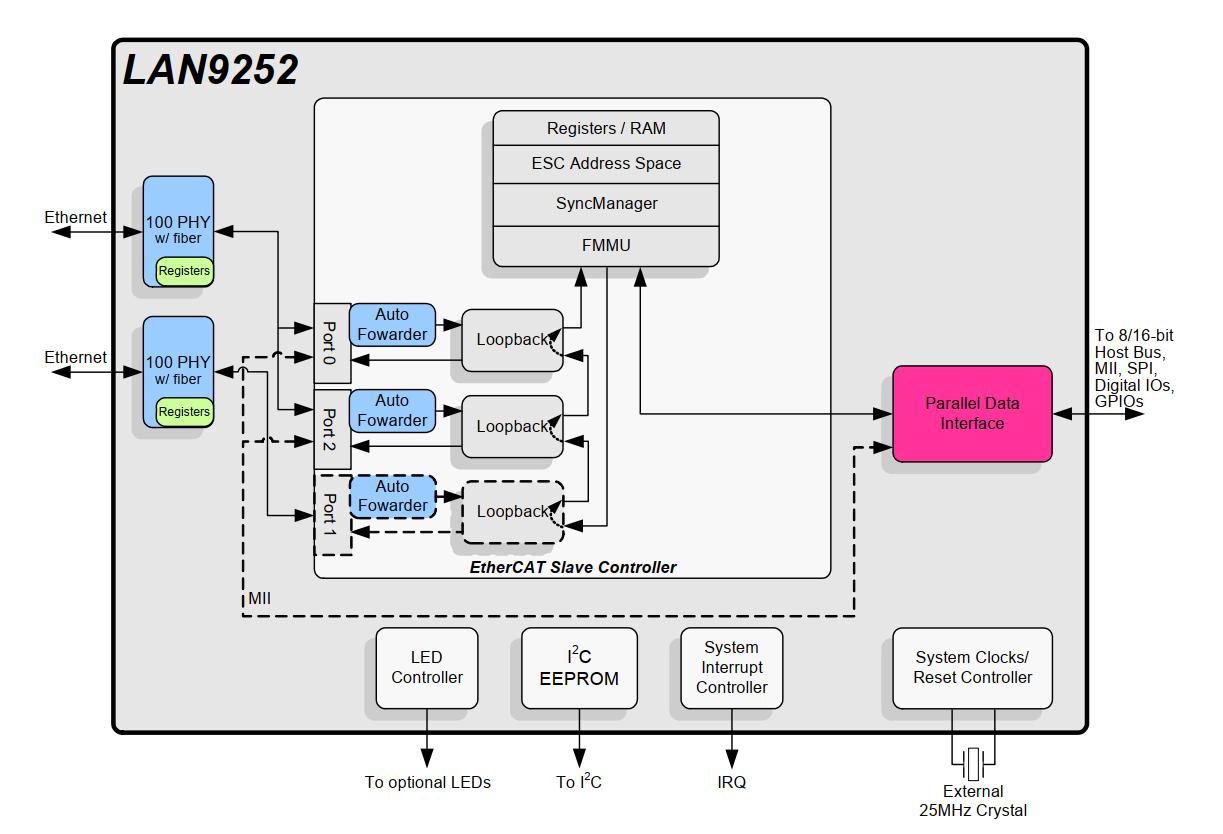
\includegraphics[width=\textwidth]{imgs/impl-lan-structure.PNG}
  \caption{Internal structure of the LAN9252, notice the PDI and EEPROM's location.}
  \label{fig:lan92struct}
\end{figure}


\subsection{Development}

Once explained the general information regarding the Communication Profile, the library and the hardware, the following lines will list and
expose some of the most relevant information during the integration. 

\begin{description}
\item[Porting of low-level functions] All the variations of functions for reading and writing ESC's registers (directly and non-directly addressed)
      are needed to be defined. HAL libraries can be used, DMA, interruption or timeout based, nevertheless, tests are required for library performance.
\item[First tests] Before integrating the SOES library, basic tests with self written functions over SPI-DMA and SPI-timeout were compared by accessing
      to test registers available in the LAN9252.
\item[Selection of the features] At the same time, in order to have the SOES library running, the features it includes needed to be selected depending on
      their usage, complexity and other things. For example, there are some MCUs that include EEPROM memory, that is mandatory for the implementation of FoE service.
      In the case of the STM32F4xx that does not have any EEPROM, the flash memory can be used instead. However, this approach represented extra effort
      in this early stage of the development. Therefore, in addition to the initial requirements, this service was avoided and the SOES integration could
      continue in a relatively lighter way.
\item[Second tests] Once understood the logic behind the library, SPI commands are sent in interruption mode and communication with the ESC was tested for the
      directly addressable registers, namely the ones related to configuration of the PHY and general chip configuration, not the ESC functions.
\item[Third tests with the Master] At this stage a compliant EtherCAT Master was configured through a PC running TwinCAT3. 
      In order to ensure a reliable configuration two different EtherCAT devices were connected synchronizing their data with the Master. Namely, 
      a commercial 3-Phase Motor Controller and an in-house multi-protocol end-effector tool. For those different devices, data structures were declared 
      and very simplistic update loops were programmed within the XAE (TwinCAT) environment using \emph{SText} programming language.
\item[Creation of an ESI file] Since the EtherCAT Core registers are indirectly addressed and only available till the ESC has been firstly readout by a 
      Master, the ESI file needs to be defined and loaded to the EEPROM of the ESC. In this way, the Master can compare and verify its compatibility and 
      the described Data Object Dictionary. The latter is closely related with the mentioned ESI file, since they are both in the same file. 
      The available information and tools provided by Beckhoff are originally designed for Beckhoff's ET1100. Microchip in turn provides some test
      examples running on PIC32 MCUs in specific development boards. The challenge was to analyze the available information to adjust the configuration
      files to the LAN9252 interfacing with the STM32 MCU. In ~\ref{app:esi_file} the main structure of the created ESI file can be consulted.
\item[Object dictionary] The object dictionary was also included in the SOES library, matching it to the one contained in the ESI file, but mapped 
    according to the few documentation available of SOES.
\item[Fourth tests] Longer tests and configuration loops were located at this stage due to the deepening on the protocol. 
Constant comparisons between the data read by the Master and the data received by the MCU host took place.
\end{description}


\section{Device State Machines (DSMs)}\label{sec:statemachines}

% Guideline
%     Introduction
%     SMS and interaction    
%     Synchronization approach, UPPAAL representation
%     Introduce the SMs what things have to be taken into account for the scheduling and prioritization

In order to have a deterministic behavior of the embedded system, a set of State Machines (DSM) -not to be confused with Synchronization Manager- 
were proposed and implemented as part of the project library. 
The DSMs software implementation follows a \emph{switch case} comparator approach, since it was simple, yet effective and flexible enough, 
to work during the prototype. 
These characteristics were very important, since the DSMs structures were in constant change as the integration of new libraries 
and the functionalities developed. 
The proposed DSMs are as follows and the diagrams can be reviewed in Appendix \ref{cha:state_machines}.

\begin{description}
\item[LED] Initializes and updates periodically the RGB value of the LED Rings. See in Fig.~\ref{fig:dsm_led}.
\item[Event Handler] Its purpose is to react to notifications or errors that could appear within other DSMs and notify to update the LED rings in accordance.
                    The approach of having defined this DSM was mainly thought for fault handling and will be the base for the inclusion of future features, e.g.,
                    receiving commands or interruption requests from any of the interfaces. See in Fig.~\ref{fig:dsm_event}.
\item[ECAT] Initializes the EtherCAT communication and activates the SOES App. It is important to mention, that this DSM is rather focused on synchronization 
            with the SOES state machine. The latter changed as the development advanced, since the native infinite loop the SOES library is based on had to be adapted.
            The two involved DSMs can be seen in Fig.~\ref{fig:dsm_ecat}.
\item[Temperature] Initializes and runs the temperature related functions. It relies primarily on the open-source library described in Sect.~\ref{sec:temperature}. 
            The DSM can be seen in Fig.~\ref{fig:dsm_temp}.

\end{description}

As to the representation of the DSM, it is important to consider the general two approaches for Finite State Machines, namely Mealy and Moore, since both 
of them provide advantages while abstracting the desire logic of the different functional blocks. In this rather practical approach the formalities are not fully
met, for instance, to choose strictly for transitions dependent on the state and inputs with actions, but using exit actions as part of each state, when it is convenient.
There are though transitions that explicitly executes a synchronization edge. This flexibility was opted due to the inherent interconnection of the DSMs
as they are not fully independent. To meet a suitable representation, the previously said is integrated with the approach of UPPAAL 
software to model timed automata and the reader is invited to look it up in \cite{uppaal_tutorial}.
As a summary, since the modelling of automata for real time systems demands a synchronization feature, this is represented and attached to the edges between 
locations (location in the sense that a state is a location constrained to valuated time and other variables) with the symbols $?$ and $!$, the former acting as 
a wait action, while the latter as a notification. Those, clearly can be understood as signals between different threads.


\subsection{Scheduling}\label{sec:scheduling_intro}

%Guidelines
% introduction
% --------------------
%     Mention the scheduling apporach of RTOS
        
%         List of proposed threads and description of them (only proposal)
%         Priority based, fixed and not based on Execution times
%            >> Time proposed for each one, mention that it is also configurable. 
%           SPI speed calculation?
%         This is a Table
     
% ---------------------This is in results-----------------------------------
%     Problems in the implementation 
%         Priority of each task + timer priority
%             Solutions + Task manager
%          Present the final table of threads
%         explains events its problems with timers, etc    
%             Solutions
%     List of resources that might demand mutex
%             List of general variables
%         Regardinf the synchronization: How the OS prevents from problems?
%             solutions
%           Future improvement (3 items for OS debugging)

In the present section, the main points regarding thread management and scheduling is presented.
All the DSMs were implemented as \emph{Threads} using CMSIS-RTOS on STM32. All threads have fixed priorities and the desired execution time
(\emph{release}) is controlled to each thread through the OS-native delay function. The previously mentioned function is not to be confused 
with the \emph{HAL} version of it, since using HW-related functions while executing an OS is conveniently avoided. The OS-function allows 
the scheduler to allocate CPU resources to any next-priority tasks. For further information regarding HAL and CMSIS implementation of delay
can be seen in ~\cite{hal_drivers} and in section \emph{Time Management} of \cite{cmsis_doc} respectively.
The time constraints are defined as \emph{desired}, since the system is
non Safety-Critical---recall the safety specification in Table~\ref{tbl:tech_specs}; hence, it has no hard real time constraint and the overall 
execution follows a best-effort approach. This, however, opens the door to further improvement in the sense of characterizing and optimizing
the reliability and task execution; the latter will be commented in Sect.~\ref{sec:scheduling_results}. 

In Table ~\ref{tbl:threads_generals} are presented the basic timing requirements depending on the functionalities of each DSM related to the thread.
Each parameter that sets up the duration can be changed in a header file, see the Appendix~\ref{appx:code}, and the individual functionality can be 
reviewed in the previous DSM section.
%**Here comes a table with the priority for each task**
\begin{tuhhtable}
    \begin{tabular}[tp]{L{.3\textwidth}C{.3\textwidth}}
      \THc{1}{c}{Thread} &  \THc{1}{c}{Release period (\si{\milli\second})} \\
      \abovebodyrule
        SOES APP SDM    & \numrange{5}{10}     \\\TRc
        LED SDM         & \num{33}    \\
        ECAT SDM*        & \num{100}     \\\TRc
        Temperature SDM & \num{1000}     \\
      \belowbodyrule
    \end{tabular}
    \caption{Basic timing requirements for threads, deadlines are rather desired since the device is non Safety-Critical. \emph{*ECAT SDM 
        is mainly event driven, nevertheless, in the connected state it has a periodic update}}
    \label{tbl:threads_generals}
  \end{tuhhtable}

A final list of priorities and threads is presented in the Table~\ref{tbl:threads_final} within Chapter~\ref{sec:results}.

%RAte monotonic oder deadline monotonic???
%EDF ----Scheduling , is this for dynamic priorities?


\section{PCB development}
%Guidelines
%   Purpose : to have a prototype
%              Altium design
%               Create a framework for hardware development
%   Based on NUCLEO 
%   Altium 3D design
%  ! Foto of real one 
%       List of issues with a simple solution
%       List of improvements
%   
%   -------------Not necessary
%   Table with, number of layers, size
%   BOM, connectors, pcb specifications
In this section straightforward information regarding the manufacturing of the PCB proposal is given.
The schematics and PCB layout can be consulted within the Appendix~\ref{appx:pcb}. The main idea around this design was introduced in Sect.~\ref{sec:pcb_proposal} 
and has the purpose of providing experience in embedded hardware design and a base work for coming projects, where
the functionalities of this prototype will be merged with other boards. Therefore, to have a physical prototype to recognize
possible opportunity areas, such as physical connectors, sizes, power source quality and signal integrity, is a corner stone for any 
future design.
The overall stages of this design are as follows:

\begin{description}
\item[Design] Altium Designer was used to prototype the PCB for this project. During the process the first approach was
                based on the open files for both the NUCLEO-F446ZE Development Board by STM and LAN9252-EVB-SPI by Microchip. By analyzing
                the general diagrams and selecting and adapting the different modules to adapt the requirements was the main challenge. To ensure
                usage of less extra devices as possible, two voltage regulators were included for \SIlist{5;3.3}{\volt}.
                To meet the routing needs a four layered PCB was selected. The final 3D model can be seen in Fig.~\ref{fig:pcb3d}.
\end{description}

\begin{figure}[ht]
    \centering
    \subfigure[ACB 3D view top]{\label{subfig:pcbtop}{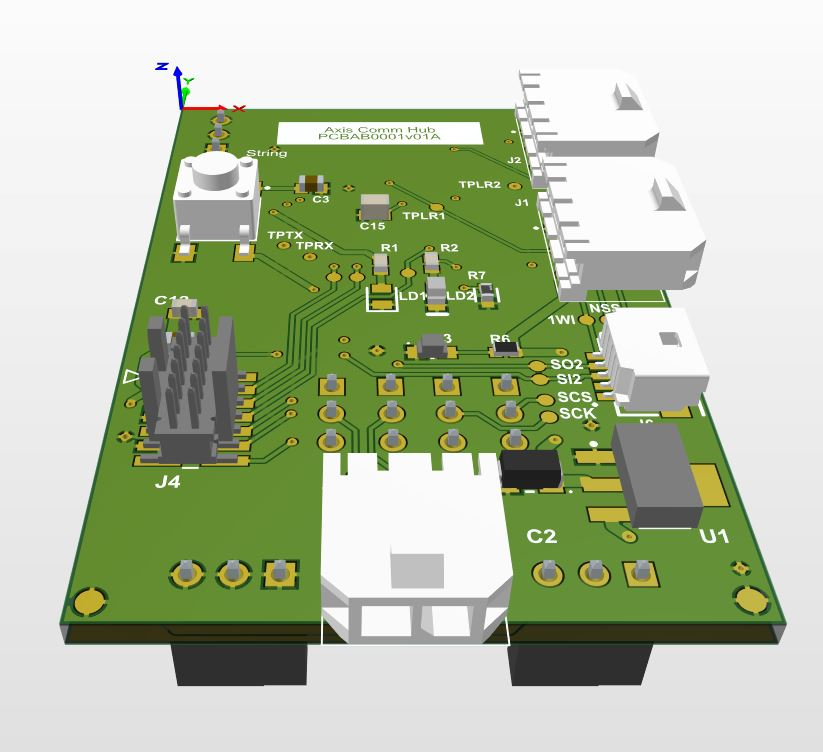
\includegraphics[width=0.4\textwidth]{imgs/pcb3d_1.JPG}}}\hfill
    \subfigure[ACB 3D view bottom]{\label{subfig:pcbbottom}{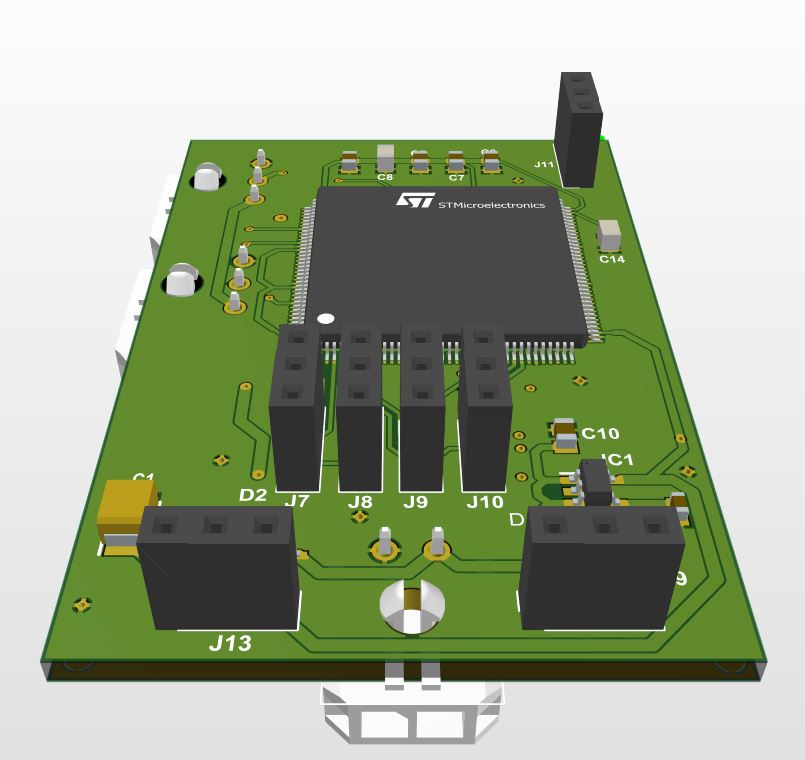
\includegraphics[width=0.4\textwidth]{imgs/pcb3d_2.JPG}}}
    \caption{3D model generated by Altium for the final design.}
    \label{fig:pcb3d}
\end{figure}


\begin{description}
\item[Manufacturing]    Due to practical reasons, the board manufacturing process was in charge of an external PCB manufacturer. In respect
                to soldering, it was made in-house.

\item[Testing I] The overall integrity and functioning of the Power-on and SWD-Programming of the STM32 MCU via SWD/JTAG connector on-board was firstly tested with good results. 
\end{description}

\begin{description}
\item[Testing II] By this stage, the readout of directly addressed memory space, specifically test and ID register, of the LAN9252 had been already done
                    with the NUCLEO board. In this manner, the code was programmed onto the ACB and so, the SPI communication gave good results. Moreover,
                    the PWM Outputs over the two channels for WS2812 LED control and the 1-wire connection were also physically tested.  
\item[Testing III] This phase is an ongoing task, since depending on the development of all the features, communication speeds and hardware 
                configurations, different scenarios are continuously emerging. A deeper analysis will be taken into account for next versions.
\end{description}




\chapter{Results}\label{cha:results}

In this chapter it is presented a set* of evidences from the final results. And it is summarized the challenges and further improvements that can be considered in later versions of the \emph{Axis Communication Hub}.

\section{Photographic evidences*}
\begin{description}
\item[Wireshark trace] **Insert captures of the EtherCAT frames/datagrams for initialization or a change of state INIT-OP
\item[TwinCAT] **Insert a capture of XAE showing the EtherCAT Slave within the EtherCAT tree. Moreover, the data types declared in SText to update in free-run mode the values sent by the Slave device.
\item[Board peripherals] The figure that shows two LED strips and 10 temperature sensor connected to the Board. **inserts the figure**
\end{description}

\section{Challenges and accomplishments}\label{sec:challenges}
\subsection{LED Control}

An open point which did not represent an obstacle for the project, but keeps the door open to further improvement is the possibility of using more than one channel per PWM generator. The reason was this was not implemented lays on the time required for testing. The straightforward option is use one DMA channel and one PWM Channel per ring, as the MCU host contains several DMA channels* *here comes a reference to a table* this does not represent a problem. Nonetheless, it could be argued that with the same PWM X generator more channels could be controlled if they are updated in a row; this is, updating the Y number of LEDs within the Ring1 using DMA stream attached to PWM X, then switching the channel to CH+1 and, using the same DMA stream, update the Ring 2 and so on. This approach would imply apparently longer times but if the Rings are taken as a fraction of the same buffer then it's the same time*. This could also lead to the discussion about using two streams at the same time for a total of 8 Rings with only two PWM generators and two DMA streams, since they rely on independent hardware -one of the main characteristics of the DMA modules-. The optimization of this LEDs control is not part of the scope of this project but the following links resulted interesing.*add the link*

*Mention the priority of the functionalities << important, maybe in introduction

\subsection{Temperature acquisition}

*here comes the problematic about the parasistic power supply* and the polling of the hardware status, this means, there is more space for improvement with YIELD or timeouts from OS funcitons.***


\subsection{SOES}

Understand the variations between Little/Big Endian within buses. That the library is based on polling by one by one the unique FIFO register of the ESC, such that the PDOs can be written and read in the PD RAM, as it was thought that a direct access to the RAM would permit the User Address Space of the MCU to be extended and the access then would be transparent for manipulating the data,  and that the SM would permit only the safe access from the Master device to read/write the same address space. It could be then understood that there is a significant delay that van be even measure, that in some papers is determined as "Stack Delay" which in this case *Reference the paper of the design of the communication/delay analysis*.
The advantages of reducing it through the implementation of the SQI or the HSI interface -which at the end does not have that much purpose since for achieving less delays the FPGA or ASIC maybe implemented-. The question, is it still sensible to develop EtherCAT devices with this approach or should it be switched completely to the FPGA and ASIC approach. An analysis considering costs and other things could be then carried out. ***
**Making available the Szstem Interrupt Controller without polling would also increase the performance of the application, this can be aimed in next versions where physically the the pins are connected to the Host MCU.
**A brief analysis of the bandwidht achieved as the bandwidth necessarz to make sensible a change of PDI would make sensce, since the HBI****reference to internet or anz specification of HBI*** is mainly foucsed to Board-To-Board connections or communication between ASICS, hence  4Gbps per pin die-to-die connectivity with low latency may not be needed at all *https://www.synopsys.com/designware-ip/interface-ip/die-to-die.html**.
**Important to mention is the HBI only helps exchanging process data, so it could be implemented for applications where data chunks are needed to be transmitted at high bandwidth since it is a direct fifo access to the ESC's SRAM.
**Here should be also commented the problems by reading and writing, mainly writting due to the noisy medium (cabling).

\subsection{State Machines and RTOS}
\subsection{PCB and hardware}
\subsection{Challenges}
The overall functionalities of the PCB were achieved from the first attempt, leaving only one disadvantage that appeared until the tests for the readout of temperature sensors were in the final stage. According to the library integration process commented in ~\ref{sec:temperature}, during the first month a rather simplistic approach was coded to have access to the temperature values. The final library that was included made use of the UART peripheral in a full duplex mode, which means that two independant pins were explicetely needed, namely RX and TX. Since, within the first approach only one GPIO was being driven, the current physical routing of the board was not appropiate to test properly the one-wire communication. Nonetheless, arrangements werd carried out to use the UART RX/TX pins available in the JTAG connector. This approach was marely for testing and will be corrected in any further development out of the scope of this Project Research.

\subsubsection{SPI communication}
During the final tests some communication errors appeared that were tracked back to the following conditions: %TODO Investigate if this can be called failure modes
\begin{description}
    \item[Voltage drops] The on-board Low-Dropout voltage regulator* LDO that provided 3.3 V had random failures, where 
    the output voltage was from 3.28 to 3.29 V. This caused that the LAN9252 chip was not always ready to work as intended. 
    This behaviour increased from not-happening to failed completely to start. The mentioned condition obly affected the ESC functionalities,
    whereas the host MCU worked realiably. To revert this failure mode, an external 3.3V power source was used to continue
    the current tests. 
    \item[Noisy channels] While troubleshooting the communication problems mentioned above, an SPI communication
    test was carried out, such that the effects of different configurations could be characterized. It was concluded that
    the higher frequencies the SPI was set up, the greater communication faults appeared, leading to error states in the 
    internal SMs. Moreover, even within rhe stable range, the higher frequencies were not implying shorter execution times.
    A summary of this observations are presented in the table \ref{dummy}.  
\end{description}
Regarding the no-improvement of the execution time at a high-speed SPI configuration, the figure \ref{dummy} shows 
a relatevely constant software delay within the words being sent over the SPI bus. Therefore, it does not matter how fast the
words are sent, for this Software delay is always present *write the order of the delay*. This emergent characteristic of
the system could be optimized as long as it is determined, whether its impact is critical on the overall throughput of the system.
The reader should take into consideration the rather small amount of data and the refresh speed of the overall system. However, this
could be a stating point for improvement of the SOES stack, for those SW delays can be approached by using a fixed sending buffer
through DMA instead of the usage of the native* API functions that send word by word. A further evaluation of the worthiness*
of the library changes may be needed.*
The above mentioned challanges are addressed within the proposals for improvement presented in the section \ref{sec:improve}.

\chapter{Conclusions}\label{cha:conclusions}

% Overall status: Board and basic SOES features ready for further EtherCAT development.

% Even though, there have been delays due to the libraries being ported, and channels being noisy before having the PCB working, we're in a stage where we can ensure that the PCB manufactured and ported libraries allow to further develop an EtherCAT compatible application. Therefore, in the following calendar days the following tasks will be priorized to complete the main tasks:





% Bibliography
% if you have cited papers that are not referenced, but important for your work,
% uncommented the following line; however, this should generally by unnecessary
% and hints at improper citing.
% \nocite{*}

\tuhhbibliography{thesis}


% Appendix
% Feel free to add additional appendix chapters (e.g., measurement setups, etc.)
%Code should be added as an appendix?
\begin{tuhhappendix}
  \chapter{Device State Machines (DSMs)}\label{cha:state_machines}
%LED control
\begin{figure}[h]
    \centering
    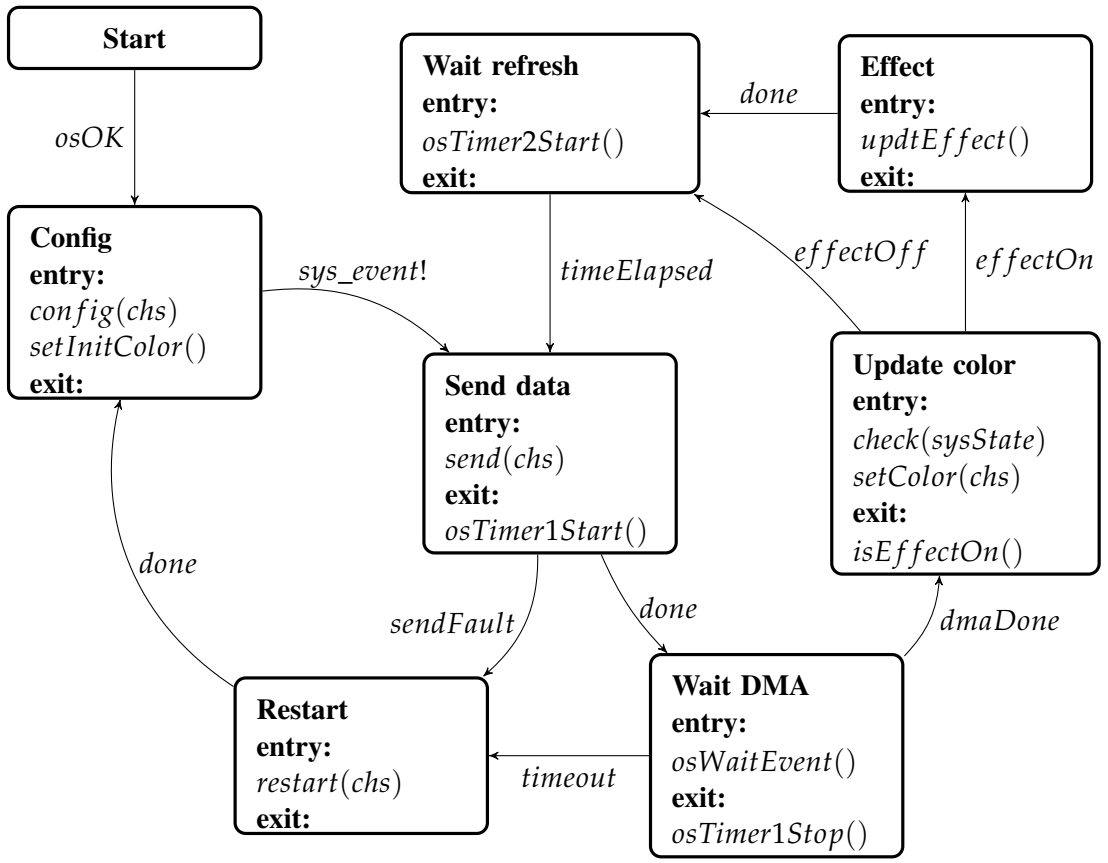
\includegraphics[width=\textwidth]{imgs/dsm_led.png}
    \caption{DSM for LED control functionality.}
    \label{fig:dsm_led}
\end{figure}
%event handler
\begin{figure}[h]
    \centering
    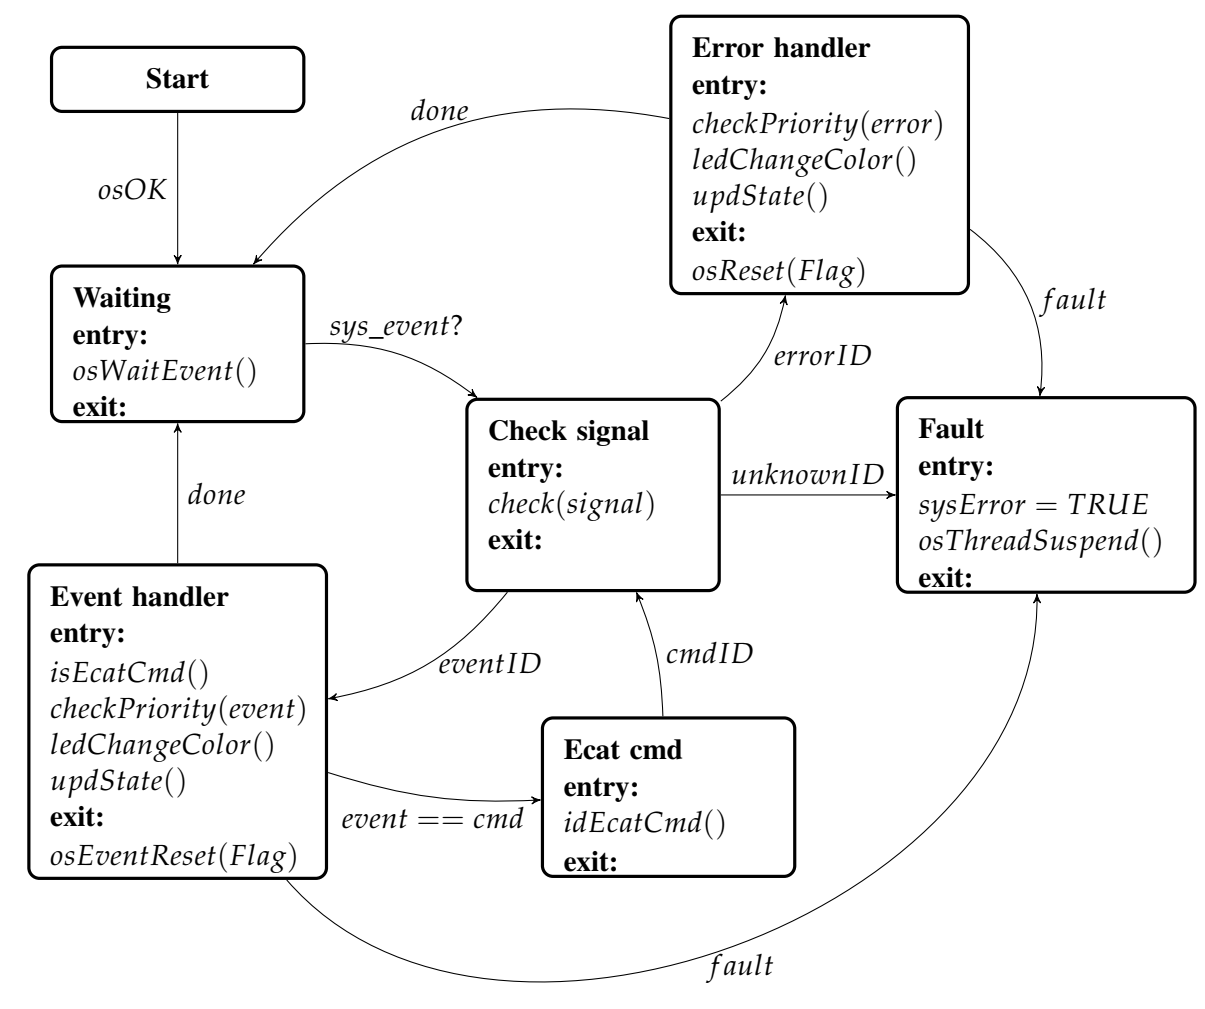
\includegraphics[width=\textwidth]{imgs/dsm_event.png}
    \caption{DSM for Event handler functionality.}
    \label{fig:dsm_event}
\end{figure}
%ecat
\begin{figure}[h]
    \centering
    \subfigure[Synchronization state machine.]{\label{subfig:ecat1}{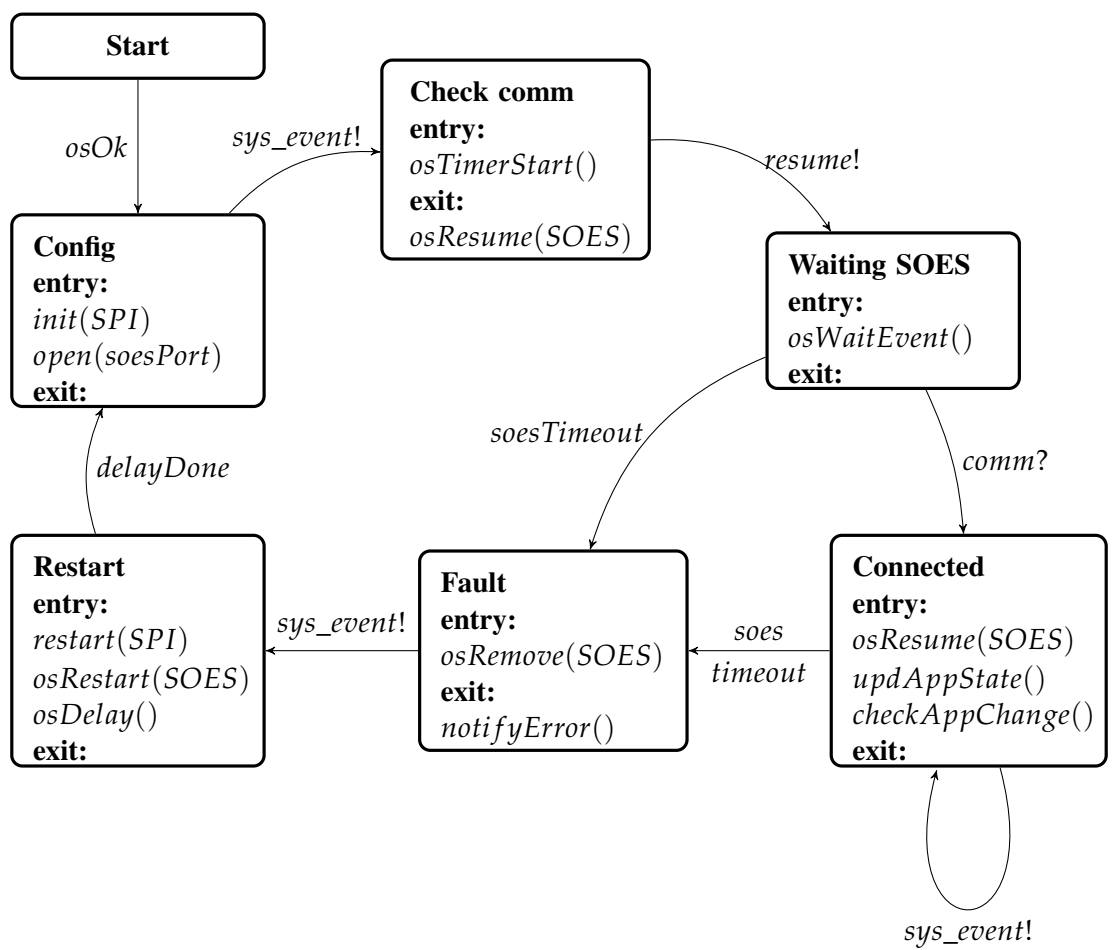
\includegraphics[width=\textwidth]{imgs/dsm_ecat1.png}}}\\
    \subfigure[SOES application state machine.]{\label{subfig:ecat2}{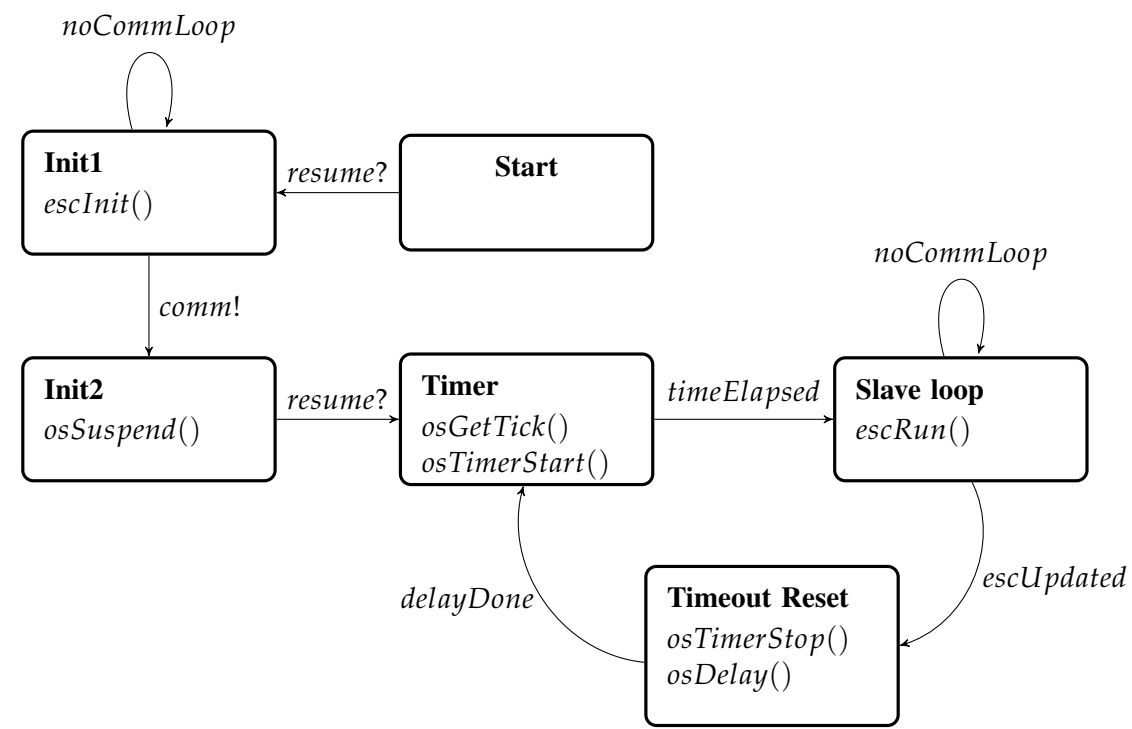
\includegraphics[width=\textwidth]{imgs/dsm_ecat2.png}}}
    \caption{DSM for EtherCAT functionality.}
    \label{fig:dsm_ecat}
\end{figure}
%temperature
\begin{figure}[h]
    \centering
    \subfigure[Synchronization state machine.]{\label{subfig:temp1}{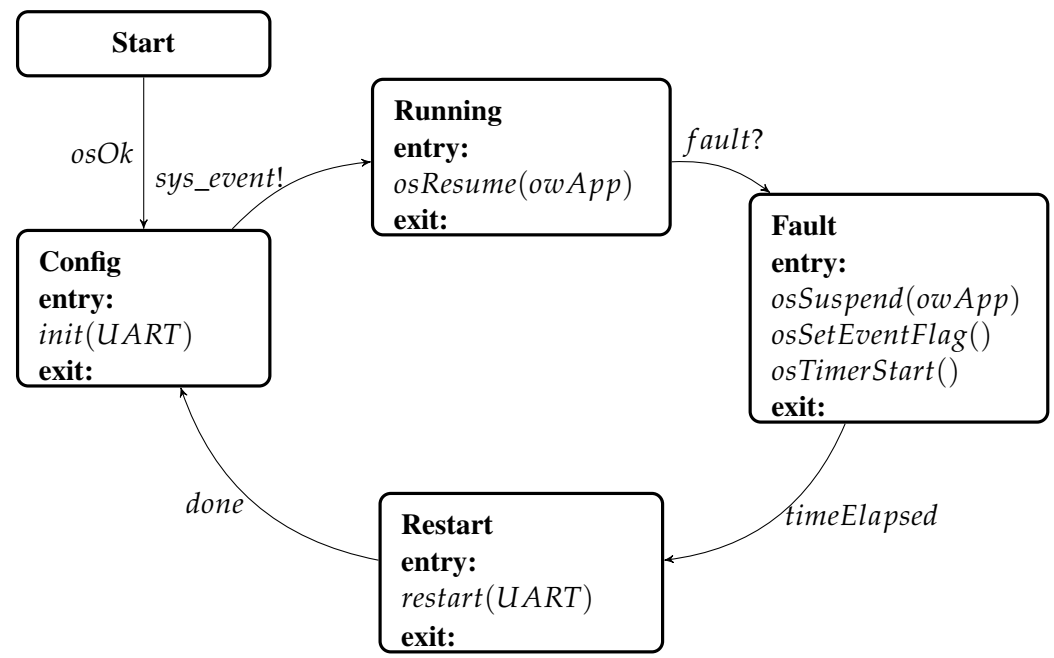
\includegraphics[width=\textwidth]{imgs/dsm_temp.png}}}\\
    \subfigure[One-wire application state machine.]{\label{subfig:temp2}{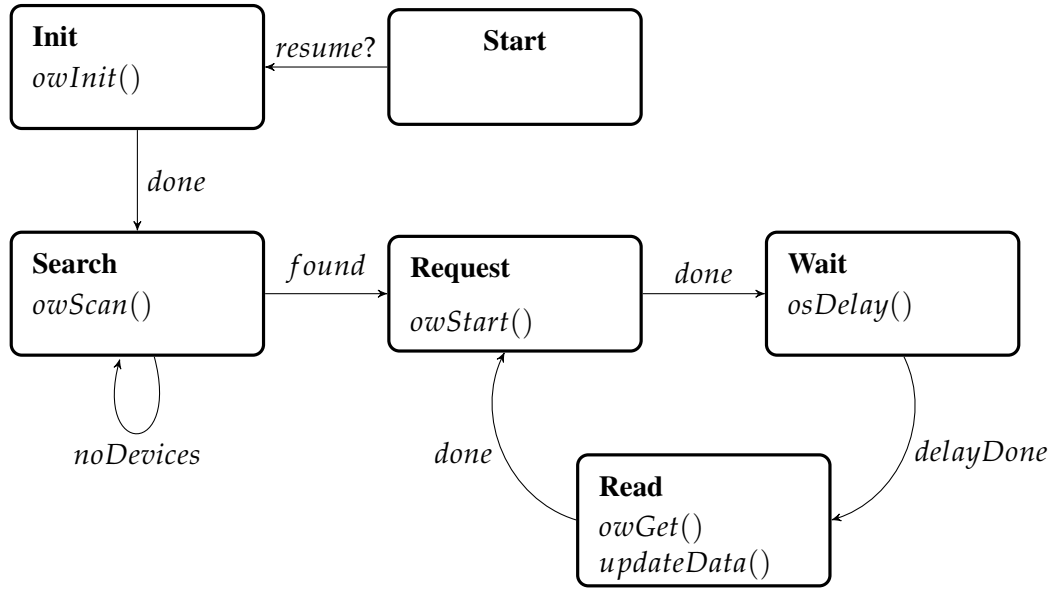
\includegraphics[width=\textwidth]{imgs/dsm_temp2.png}}}
    \caption{DSM for Temperature functionality.}
    \label{fig:dsm_temp}
\end{figure}
  \chapter{Introduction to EtherCAT}\label{sec:ecat_protocol}

As mentioned in the introduction, EtherCAT is an industrial Communication Profile developed by Beckhoff Automation GmbH that is 
standardized in the IEC 61588 under the RTE CPF. The development within this company is oriented to the use of 
open standards to increase its impact within the industry, but not only reduced to it but the overall smart cities field, in
a certain degree this approach eliminates the need for many expensive \emph{black boxes} as mentioned in ~\cite{beckhoff_automation}. %%Beckhoff_Urban_Automation_2013_e almost the introduction thing 
This implies that the interoperability of devices is almost guaranteed, at least from the specification perspective,
not only for private development centers but also for any other developer that follow the standards; if the standards 
are of public access, then this is a mean of empowerment of any group that might be willing
to create its own industrial-compatible technologies.

The OSADL emphasized in 2008, see article in ~\cite{beckhoff_vs_osadl}, for example, a vision for leading the integration
of open source in the industry by using the Linux Kernel as a certified Industrial RT (IRT) operative system for industrial embedded applications. 
Back in that day, Beckhoff Automation was involved in that discussion representing the contrary model. Nonetheless, in the last months the same company has
apparently retaken the open source initiative by the introduction of the FreeBSD compatible version of the TwinCAT Runtime---visit this newsletter ~\cite{beckhoff_freebsd}.%https://www.heise.de/newsticker/meldung/Open-Source-trifft-die-Industrie-201855.html
%**https://www.beckhoff.com/english.asp?highlights/twincat-bsd/default.htm

In comparison with other RTE profiles, EtherCAT has shown a higher performance, more flexible topology and lower costs than other field bus 
technologies. This  protocol  applies  a  master-slave  mode,  in  which  the  master  
device  uses  standard  100BASE-TX  Ethernet  adapter  and  the  EtherCAT  Slave  Controller (ESC), that implements an EtherCAT IP 
(intellectual property) core within an ASIC or an FPGA to process the frames. As  the  working  cycle starts, the  Master  
publishes a frame encapsulated a standardized 8802.3 frame. When it reaches an ESC, it analyses the address and location on the frame, decides
which parts of it are useful sections and then reads or writes data on it. As the
read-write operation finishes, the Working Counter (WKC) at the end of the frame is added by one, this way the data on the frame has been processed. 
This cycle repeats for each ESC within the topology. %Motion Control System using SERCOS over EtherCAT

EtherCAT supports almost all kinds of topology structure, such as ring, line, star and tree. The transmission speed of the interface is fixed to \SI{100}{\mega\bit\per\second}
with  full  duplex  communication.  The  network  is  able  to  connect  maximally 65535  devices  via  switch  and  media  converter.  
The  EtherCAT  system  can  update  1000  I/Os  in  just  \SI{30}{\micro\second} or  exchange \SI{1486}{\byte} contents in  \SI{300}{\micro\second}.
The previous technical data can be reviewed in ~\cite{beckhoff_datasheet} and an overview of the protocol in ~\cite{ecat_sercos}. %Motion Control System using SERCOS over EtherCAT

Important to highlight is that other CPs are also integrated as services inside the protocol, as mentioned before for 
the SERCOS specification in Sect.~\ref{sec:applications}. 
Other examples of these integrated CPs are File over EtherCAT (FoE) or Ethernet over EtherCAT (EoE), which  
make possible support a wide variety of devices and application layers in the same network.
A complete list of the communication profiles that are on hand
through the protocol's mailbox is given below, as to the overall layered integration can be seen in Fig.~\ref{fig:ecatprofiles}.
\begin{itemize}
    \item CoE: CAN application protocol over EtherCAT
    \item SoE: Servo drive profile, according to IEC 61800-7-204 (SERCOS protocol)
    \item EoE: Ethernet over EtherCAT
    \item FoE: File Access over EtherCAT (HTTP,FTP,etc)
    \item AoE: Automation Device Protocol over EtherCAT (ADS over EtherCAT)
\end{itemize}

\begin{figure}[ht]
    \centering
    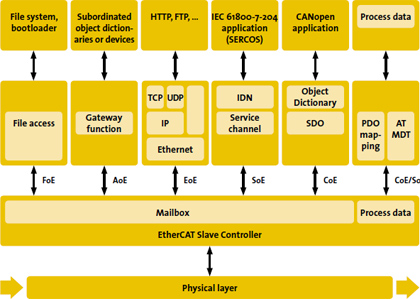
\includegraphics[width=.65\textwidth]{imgs/intro-ecatprofiles.jpg}
    \caption{Different communication profiles can coexist in the same system. Source from ~\cite{beckhoff_compatibility}.}
    \label{fig:ecatprofiles}
\end{figure}

An EtherCAT device with switch port properties using EoE would be the equivalent of the TSN compliant
switches, since they would insert any non time-sensitive TCP/IP fragment into the RTE traffic preventing
in this way the real time properties from being affected. Furthermore, the architecture of the protocol itself and
its early cooperation with the IEEE 802.1 group and the OPC Group ensure its continuous compatibility with the
standardization of TSN, OPC UA and the IoT paradigm. See the following article about compatibility \cite{beckhoff_compatibility}.%https://www.ethercat.org/en/technology.html#1.12


% *Add the image of the Ethernet frame having the EtherCAT datagram inside.
% *Explain the XAE tool and the PDI meaning
% *Quote maybe from paper section BASICS OF ETHERCAT AND PROFINET IRT Network Delay Analysis of EtherCAT and PROFINET IRT Protocols***
%** Question. What would happen if the synchronization mode within an EtherCAT network wants to be integrated to those of a TSN???


\begin{figure}[ht]
    \centering
    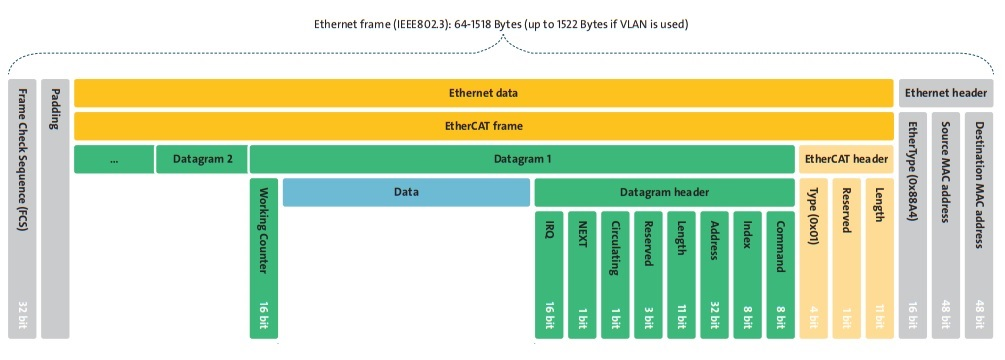
\includegraphics[width=\textwidth]{imgs/impl-dataframe.jpg}
    \caption{EtherCAT datagram within the Ethernet frame. Source from ~\cite{beckhoff_datalink}.}
    \label{fig:dataframe}
\end{figure}

\subsubsection{The data frame and the Synchronization Managers}\label{sec:synch_managers}

Besides the challenge of setting up the hardware and basic firmware for a correct data transmission between ESC and the host MCU; the description of the EtherCAT 
Slave device is a task that demands, at least, a basic understanding of the data frame exchange and how the protocol demands its synchronization. From here on, the following
topics are going to be summarized: Synchronization modes and managers.
Whenever there are Real Time constraints, and the device takes part of a control loop, synchronization modes are needed to be set correctly between the Master and
any Device present. For this task the Distributed Clocks (DC) are need to be synchronized. See the section 20 in ~\cite{beckhoff_enhancements}. %ETG.1020 - Synchronization and ETG.2000 - DC

There are three synchronization modes:  
\begin{description}
    \item[Free Run] Application is triggered by local clock and runs independently of EtherCAT cycle. 
    \item[SM-Synchronous] Application is synchronized whenever there are process data being written to the Synchronization Manager 2 (SM2).
    Moreover, any event generated by the Master is mapped onto an internal register or physically triggering an IRQ Pin of the ESC. 
    \item[DC-Synchronous] Within this synchronization mode the frame jitter can be even reduced down to \si{\nano\second} and use two different synchronization
    units within the ESC, namely the SM2 and SYNC/LATCH UNIT. 
\end{description}


\begin{figure}[ht]
    \centering
    \subfigure[Free Run]{\label{subfig:syncm1}{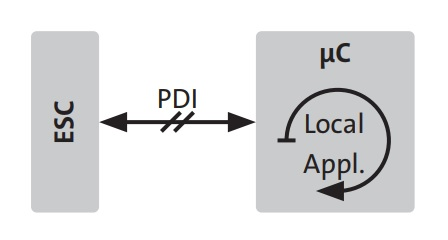
\includegraphics[width=0.3\textwidth]{imgs/impl-sync1.jpg}}}\hfill
    \subfigure[SM-Synchronization]{\label{subfig:syncm2}{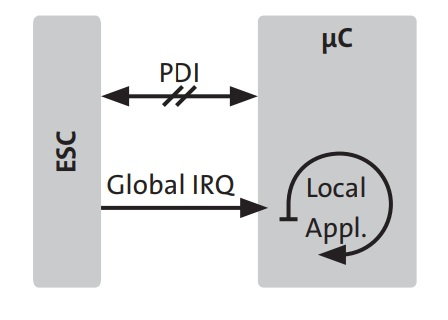
\includegraphics[width=0.3\textwidth]{imgs/impl-sync2.jpg}}}\hfill
    \subfigure[DC-Synchronization modes]{\label{subfig:syncm3}{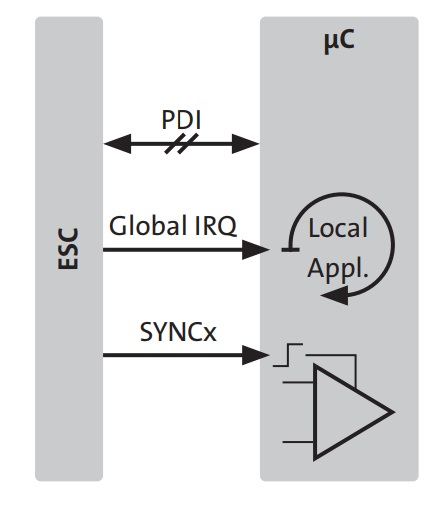
\includegraphics[width=0.3\textwidth]{imgs/impl-sync3.jpg}}}
    \caption{Synchronization modes. Definitions can be reviewed in depth within ~\cite{beckhoff_overview}.} %EtherCAT Device Protocol poster from EtherCAT resources
    \label{fig:syncmodes}
\end{figure} 

Synchronization Managers 1,2,3---as many as the hardware includes---(sometimes referred as SMXs) coordinate access to the ESC 
memory from both sides, Master and
Host MCU through the Process Data Interface (PDI). In case of process data communication it ensures that process data objects (PDO) 
can
always be written to the memory by EtherCAT and can always be read in the PDI side and vice versa (3-buffer mode). 
SyncManager 2/3 length is equal
to the Data Object lengths defined for receive and transmit data chunks respectively. SyncManagers are explained in detail in ~\cite{beckhoff_datalink}. %ETG.1000.4 Sync manager
The mapping of the process data objects within the Ethernet Frame can be seen in figure \ref{fig:dataframe} and \ref{fig:pdomapping}.
The correct setup of the SMXs ensure the consistency of the data and needs to be linked correctly depending on the characteristics of each ESC type,
 and SW Stack that are being used, this information is also linked to the CoE Object Dictionary (OD) and EtherCAT Slave Information (ESI) file.
\begin{figure}[ht]
    \centering
    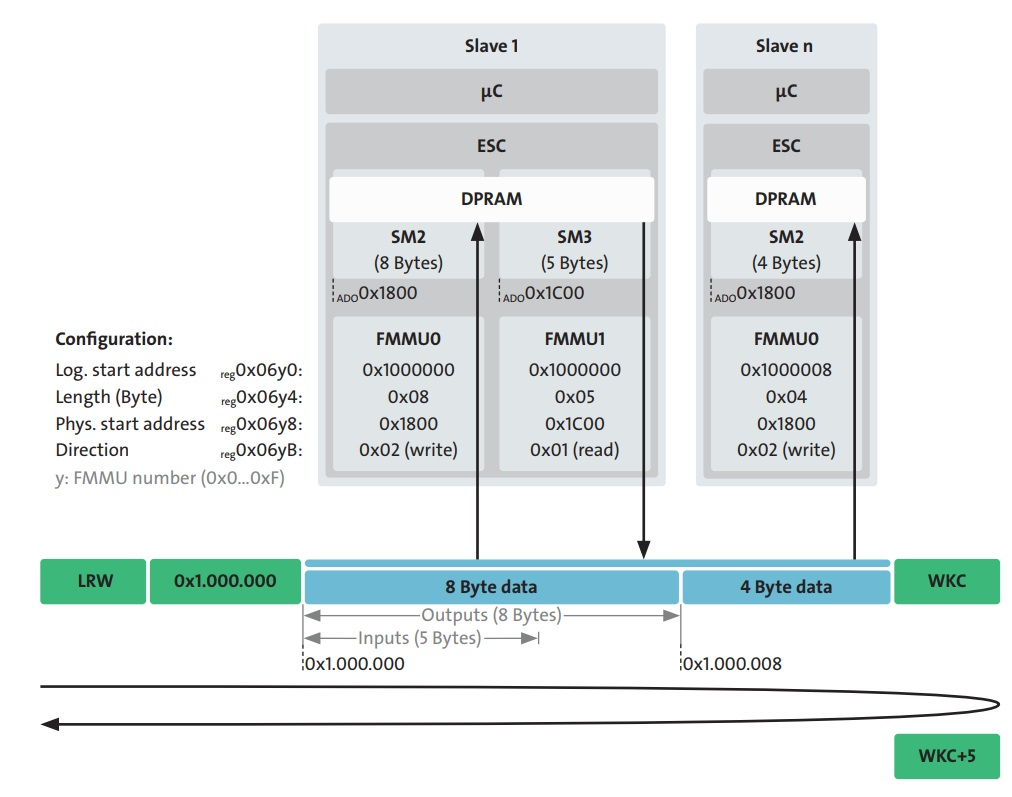
\includegraphics[width=.85\textwidth]{imgs/impl-dataframe_pdo.jpg}
    \caption{Depending on the different states of the Slave, there will be different data frames being exchanged with the Master. 
    The above one corresponds to the PDO which is updated continuously by the SM2/3 during Operation State (OP). Resource from SDO section in ~\cite{beckhoff_applayer}.}
    \label{fig:pdomapping}
\end{figure}
  % \chapter{PCB drawings and layout}\label{appx:pcb}

**here comes  the electrical diagrams and the pcb layout exported by Altium**

  % 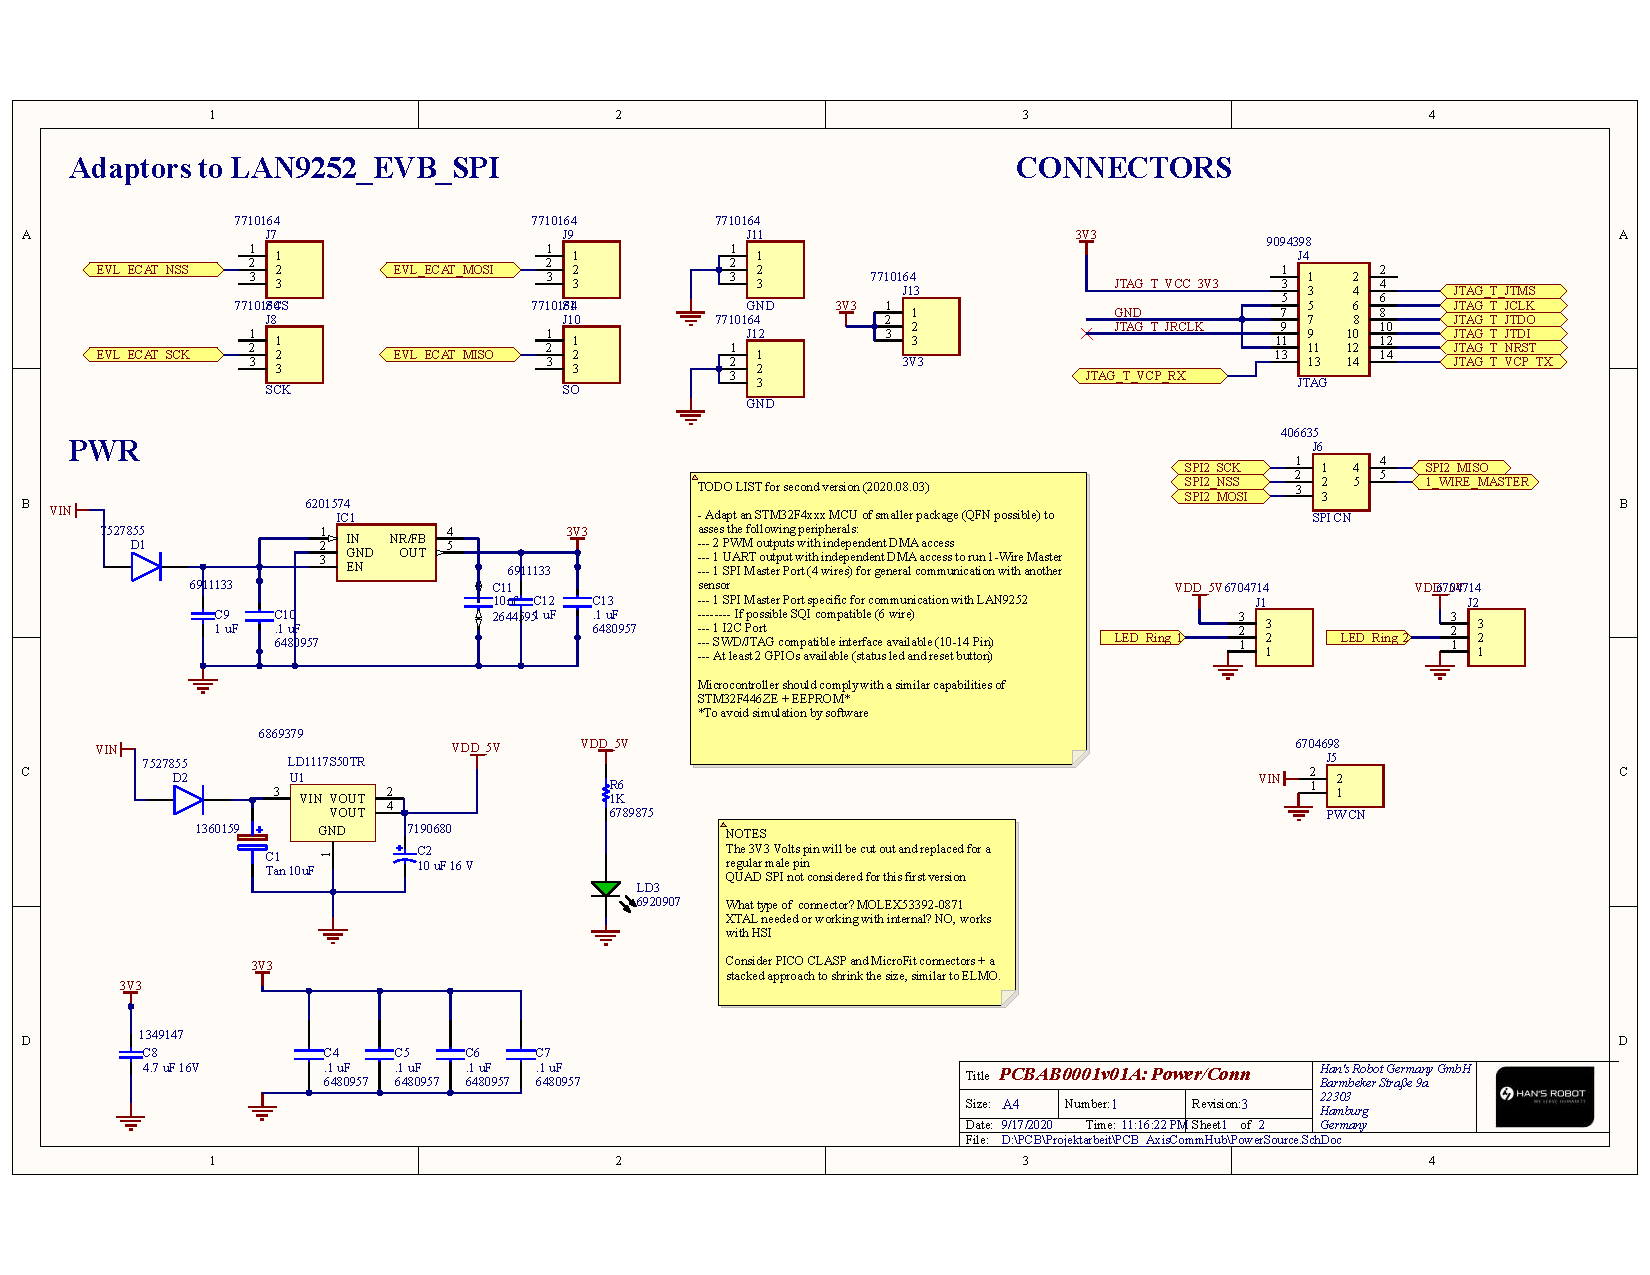
\includepdf[pages=-,landscape=true]{imgs/Schematic Prints_color.pdf}
  % \chapter{Source codes}\label{appx:code}
% This appendix shows the source code which was self written SMs and auxiliar wrappers. For any other code, namely the one-wire and soes library, since 
% they are under the GNU* license, it is easy that the reader look for oneself the code:
% \begin{description}
%     \item[LED WS2812b Driver] Original version only for one channel and suited for **add the ST family** << ** mention in the challenges \ref{sec:leds}
%         that there was a DMA incompatibility within this two families. **refer to the porting guide provided by ST.
%     \item[One-Wire generic driver] Original compatible version which includes a sample that runs in a infinite while-loop.
%     \item[SOES Library] Original version without the low level functions. << *** Mention that originally the support for ST is not provided but only for: **look 
%         the processors natively supported. \ref{sec:soes}.
% \end{description}
This appendix enlists the fundamental source codes within this implementation. The order is as follows:
\begin{itemize}
    \item Configuration header file for the main features where the full list of errors and events can be seen in ~\ref{lst:definitions}.
    \item Code for the creation and configuration of threads plus some auxiliary functions in ~\ref{lst:generalSM}.
    \item Main code for the Event Handler in ~\ref{lst:event}.
    \item Main code for the ECAT DSM in ~\ref{lst:ecatSM}.
    \item Main code for the SOES DSM in ~\ref{lst:soesAPP}. 
    \item Main code for the LED DSM in ~\ref{lst:led}.
    \item Code for the Temperature Application in ~\ref{lst:tempApp}.
\end{itemize}

\begin{lstlisting}[label=lst:definitions,caption={Main definition and configuration header file.}]
    /*
    * AxisCommHub_definitions.h
    *
    *  Created on: Jun 11, 2020
    *      Author: Carlos Reyes
    */
   
   #ifndef AXISCOMMHUB_DEFINITIONS_H_
   #define AXISCOMMHUB_DEFINITIONS_H_
   
   
   //	General include files
   
   #include "LAN9252_spi.h"
   #include "main.h"
   
   //	Definition of peripherals
   #define	NUM_OF_SENSORS			15u
   
   #define MAX_OF_LEDRINGS			4		//	This values should be modified in the LED library
   #define NUM_OF_LEDRINGS			2
   #define NUM_OF_LEDS_PER_RING	5		//	If the number is not the same for all LED Rings, then change directly within the LED library
   
   //	Generic definitions
   #define	TRUE					1
   #define	FALSE					0
   #define FAILED					-1
   
   //	Timing for SOES
   #define SOES_REFRESH_CYCLE		20u		//in Systicks
   
   // 	Mind the following structure for event flags (See #define MAX_BITS_EVENT_GROUPS     24U)
   // | 8 reserved bits | 14 bits (16383d) error space | 10 bit individual event flags|
   
   //	Declaration of event flags (10 available)
   #define SYS_EVENT			(1<<0)
   #define LED_EVENT			(1<<1)
   #define TSENS_EVENT			(1<<2)
   #define ECAT_EVENT			(1<<3)
   #define	TASKM_EVENT			(1<<4)
   
   
   //	Offsets
   #define ERR_OFFSET				1000u
   #define EV_OFFSET				2000u
   #define	SHIFT_OFFSET			10u
   //	Declaration of errors
   #define	ERR_SYS_NONE			0
   #define	ERR_SYS_UNKNOWN			101
   
   
   #define	ERR_TEMP_SENS_INIT		 1101u
   #define ERR_TEMP_SENS_LOST		 1102u
   #define ERR_TEMP_SENS_TIMEOUT	 1103u
   #define ERR_TEMP_SENS_OVERHEAT	 1104u
   #define	ERR_TEMP_DSM_FAULT		 1105u
   
   #define ERR_LED_INIT		 	1201u
   #define ERR_LED_TIMEOUT		 	1202u
   #define ERR_LED_SEND		 	1203u
   #define	ERR_LED_OSTIM		 	1204u
   #define	ERR_LED_DSM_FAULT	 	1205u
   
   #define	ERR_ECAT_INIT			 1301u
   #define ERR_ECAT_COMM_LOST		 1302u
   #define ERR_ECAT_TIMEOUT		 1303u
   #define ERR_ECAT_DSM_FAULT		 1304u
   #define ERR_ECAT_CMD_FAULT		 1305u
   #define ERR_ECAT_CMD_SOFTFAULT	 1306u
   
   //	Definition of internal events
   #define EV_TEMP_DSM_INIT	 	2101
   
   #define EV_LED_DSM_INIT		 	2201
   #define EV_LED_UPTD			 	2211
   
   #define EV_ECAT_ESC_INIT		 2301
   #define EV_ECAT_APP_OP			 2311
   #define EV_ECAT_APP_INIT		 2312
   #define EV_ECAT_APP_NOOP		 2313
   #define EV_ECAT_DSM_INIT		 2321
   #define EV_SOES_RESPAWNED		 2331
   #define EV_ECAT_CMD_ACK			 2351
   #define EV_ECAT_CMD_LED_TOGGLE	 2352
   
   
   // 	Mind the following structure for status variable (according to size of errors and events (16383d))
   // | 14 bits last event space | 14 bits last error space | 4 bit General state |
   #define	STATUS_OFFSET_FOR_ERR	4u
   #define	STATUS_OFFSET_FOR_EV	18u
   
   #define STATUS_DATA_MASK		0x3FFF
   #define STATUS_SHORT_MASK		0x0F
   
   #define	STATUS_INIT				1u
   #define	STATUS_STARTED			2u
   #define	STATUS_NO_ERRORS		4u
   #define STATUS_SOFT_ERRORS		5u
   
   
   //	Definition of specific timeouts
   //	ECAT/SOES
   #define	ESC_INIT_TIMEOUT	5u
   #define	ESC_REFRESH_TIMEOUT	10000u
   
   //	Definitions of ETHERCAT STATE MACHINE
   //	See esc.h for ALstatus Reg
   //	e.g. ESCop
   
   //	Auxiliar definitions for HAL adaptation
   
   #define CHANNEL_FOR_LED1		TIM_CHANNEL_1
   #define CHANNEL_FOR_LED2		TIM_CHANNEL_2
   #define CHANNEL_ACTIVE_FOR_LED1	HAL_TIM_ACTIVE_CHANNEL_1
   #define CHANNEL_ACTIVE_FOR_LED2 HAL_TIM_ACTIVE_CHANNEL_2
   
   
   //	Overall test definitions
   
   #define ECAT_UPDT_PERIOD_TEST_IN_MS			10u	//1>> RT	10-15 >> Industrial RT 	100>> Non-critical variables monitoring
   #define	ECAT_CONNECTION_CHECK_PERIOD_IN_MS	10u
   #define	ECAT_CHECK_PERIOD_FACTOR			ECAT_CONNECTION_CHECK_PERIOD_IN_MS/ECAT_UPDT_PERIOD_TEST_IN_MS
   #define COMM_TESTING_TIMES					100u
   
   
   //	Taken from linux definitions and needed by SOES
   #define BIT(nr) (1UL << (nr))
   
   #endif /* AXISCOMMHUB_DEFINITIONS_H_ */
   

\end{lstlisting}

\begin{lstlisting}[label=lst:generalSM,caption={Part of the code to declare threads and other auxiliar functions.}]
    /*
    * SMs.c
    *
    *  Created on: Jun 3, 2020
    *      Author: Carlos Reyes
    */
   
   #include "main.h"
   #include "AxisCommHub_definitions.h"
   #include "SMs.h"
   #include "smEcat.h"
   
   extern osTimerId_t timerEcatSM,timerEcatSOES;
   
   /*-----------------------------------------------TASKS for SMs--------------------------------------------------------------*/
   // Task Handlers declared within the SMs.h
   
   
   uint32_t tempSensTBuffer[ 192 ];
   StaticTask_t tempSensTControlBlock;
   const osThreadAttr_t tempSensT_attributes = {
           .name = "tempSensT",
           .stack_mem = &tempSensTBuffer[0],
           .stack_size = sizeof(tempSensTBuffer),
           .cb_mem = &tempSensTControlBlock,
           .cb_size = sizeof(tempSensTControlBlock),
           .priority = (osPriority_t) osPriorityNormal,
   };
   
   
   uint32_t ledRingsTBuffer[ 192 ];
   StaticTask_t ledRingsTControlBlock;
   const osThreadAttr_t ledRingsT_attributes = {
           .name = "ledRingsT",
           .stack_mem = &ledRingsTBuffer[0],
           .stack_size = sizeof(ledRingsTBuffer),
           .cb_mem = &ledRingsTControlBlock,
           .cb_size = sizeof(ledRingsTControlBlock),
           .priority = (osPriority_t) osPriorityNormal,
   };
   
   
   uint32_t ecatSMTBuffer[ 192 ];
   StaticTask_t ecatSMTControlBlock;
   const osThreadAttr_t ecatSMT_attributes = {
           .name = "ecatTSM",
           .stack_mem = &ecatSMTBuffer[0],
           .stack_size = sizeof(ecatSMTBuffer),
           .cb_mem = &ecatSMTControlBlock,
           .cb_size = sizeof(ecatSMTControlBlock),
           .priority = (osPriority_t) osPriorityNormal,
   };
   
   
   uint32_t eventHTBuffer[ 128 ];
   StaticTask_t eventHTControlBlock;
   const osThreadAttr_t eventHT_attributes = {
           .name = "eventHT",
           .stack_mem = &eventHTBuffer[0],
           .stack_size = sizeof(eventHTBuffer),
           .cb_mem = &eventHTControlBlock,
           .cb_size = sizeof(eventHTControlBlock),
           .priority = (osPriority_t) osPriorityAboveNormal,
   };
   
   /*-----------------------------------------------AUXILIAR TASKS--------------------------------------------------------------*/
   
   /*-------------------------ECAT--------------------------------------*/
   uint32_t ecatTestTBuffer[ 192 ];
   StaticTask_t ecatTestTControlBlock;
   const osThreadAttr_t ecatTestT_Attributes = {
           .name = "ecatTestT",
           .stack_mem = &ecatTestTBuffer[0],
           .stack_size = sizeof(ecatTestTBuffer),
           .cb_mem = &ecatTestTControlBlock,
           .cb_size = sizeof(ecatTestTControlBlock),
           .priority = (osPriority_t) osPriorityHigh3,
   };
   
   uint32_t ecatSOESTBuffer[1088];
   StaticTask_t ecatSOESTControlBlock;
   const osThreadAttr_t ecatSOEST_Attrbuttes = {
           .name = "ecatSOEST",
           .stack_mem = ecatSOESTBuffer,
           .stack_size = sizeof(ecatSOESTBuffer),
           .cb_mem = &ecatSOESTControlBlock,
           .cb_size = sizeof(ecatSOESTControlBlock),
           .priority = (osPriority_t) osPriorityAboveNormal,
   };
   
   /*----------------------System Monitor--------------------------------*/
   
   uint32_t taskManagerTBuffer[ 192 ];
   StaticTask_t taskManagerTControlBlock;
   const osThreadAttr_t taskManagerT_Attributes = {
           .name = "taskManagerT",
           .stack_mem = &taskManagerTBuffer[0],
           .stack_size = sizeof(taskManagerTBuffer),
           .cb_mem = &taskManagerTControlBlock,
           .cb_size = sizeof(taskManagerTControlBlock),
           .priority = (osPriority_t) osPriorityHigh,
   };

  
   /******************************************* Extern Variables from LED Rings Multichannel *********************************************************************/
   
   //volatile uint8_t currentColors[MAX_OF_LEDRINGS];	//Global array for colors to be updated, this will be changed continuously by EventHandler/Notification //CHCKME this is shared memory
   extern volatile uint8_t dmaLed1_rcvd, dmaLed2_rcvd,refreshTimeoutLed;
  
   
   /******************************************* Variables to debug ****************************************************************/
   osStatus_t static ecatStatus,uartPrintStatus;
   uint32_t *heapObserver0,*heapObserver1,*heapObserver2;
   
   /*************************************** Var task manager ***********************************************************/
   static osThreadState_t status_ecatTestT, status_ecatT, status_evHT,status_uartPT,status_tSensT,status_ledsT, status_taskMT,status_ecatSOEST;
   osTimerId_t timerTsens;	//IMPRVME	This may be a local variable to save memory
   static uint8_t timedoutTsens;
   

   
   /*-------------------------Here start the definitions of the functions needed by SM --------------*/
   /*----------------------------------- Task Manager functions ---------------------------------------*/
   /* *
    * @brief 	This function will update the status for each task and terminate a thread if needed
    * */
   
   void taskManger(void * argument) {
   
       osStatus_t status;
       while (1) {
           if (restartTaskManFlag) {
               restartTaskManFlag = FALSE;
               osDelay(100);
               status = osThreadSuspend(ecatSOESTHandler);
               status = osThreadTerminate(ecatSOESTHandler);
               ecatSOESTHandler = osThreadNew(soes, NULL, &ecatSOEST_Attrbuttes);
               status = osThreadSuspend(ecatSOESTHandler);
               osEventFlagsSet(evt_sysSignals, TASKM_EVENT|EV_SOES_RESPAWNED);
           }
   
           status_ecatTestT = osThreadGetState(ecatTestTHandler);
           status_ecatT = osThreadGetState(ecatSMTHandle);
           status_ecatSOEST = osThreadGetState(ecatSOESTHandler);
   
           //osThreadYield();	//Yield to any other thread that may be ready
           //osDelay(1000);			//1ms update rate
           osEventFlagsWait(taskManSignals, TASKM_EVENT,osFlagsWaitAny , osWaitForever);
   
           status_ecatSOEST = osThreadGetState(ecatSOESTHandler);
           status_evHT = osThreadGetState(eventHTHandle);
           status_uartPT = osThreadGetState(uartPrintTHandler);
           status_tSensT = osThreadGetState(tempSensTHandle);
           status_ledsT = osThreadGetState(ledRingsTHandle);
           status_taskMT = osThreadGetState(taskManagerTHandler);
       }
   
       //osThreadTerminate(taskManagerTHandler);	//If ever jumps out the loop
   
   }
   
   /* *
    * @brief	This function adds the threads to be executed to the OS and the general signals
    * */
   void addThreads(void) {
       evt_sysSignals = osEventFlagsNew(NULL);
       if (evt_sysSignals == NULL){
           //Handle error
           __NOP();
       }
       taskManSignals = osEventFlagsNew(NULL);
       if (taskManSignals == NULL){
           //Handle error
           __NOP();
       }
   
       heapObserver0 = evt_sysSignals;
       heapObserver1 = taskManSignals;
   
       //	Initializing main threads
       tempSensTHandle = osThreadNew(tempSens_SM, NULL, &tempSensT_attributes);
       ledRingsTHandle = osThreadNew(ledRings_SM, NULL, &ledRingsT_attributes);
       ecatSMTHandle = osThreadNew(ecat_SM, NULL, &ecatSMT_attributes);
       eventHTHandle = osThreadNew(eventH_SM, NULL, &eventHT_attributes);
   
       //	Auxiliar tasks
   
       ecatSOESTHandler = osThreadNew(soes, NULL, &ecatSOEST_Attrbuttes);
       ecatStatus = osThreadSuspend(ecatSOESTHandler);
       taskManagerTHandler = osThreadNew(taskManger, NULL, &taskManagerT_Attributes);
   
       sysState = STATUS_INIT;
       //Debug tasks
       //eventTesterTHandler = osThreadNew(eventTesterTask,NULL,&eventTesterT_Attributes);	//Pending This task could start before the system is ready
   }

\end{lstlisting}

\begin{lstlisting}[label=lst:event,caption={Main source code for Event Handler DSM.}]
    /*
     * smEvH.c
     *
     *  Created on: Jun 26, 2020
     *      Author: Carlos Reyes
     */
    
    
    #include "SMs.h"
    #include "smEvH.h"
    
    
    //External variables
    
    
    /*
     * @brief Sate Machine for error/event handler
     *
     */
    
    void eventH_SM (void * argument) {
    
        uint32_t status,flags;	
        uint16_t event_data;
    
        while(1) {		//Infinite loop enforced by task execution
    
            switch (evH_step) {
            /*-------------------------------------------------------------------*/
            case	evh_init:
                evH_initFlag = TRUE;
                evH_step = evH_waiting;
                break;
            /*-------------------------------------------------------------------*/
            case	evH_waiting:
                //	entry:
                status = osEventFlagsWait(evt_sysSignals, SYS_EVENT, osFlagsWaitAny, osWaitForever);
                //	exit:
                evH_step = evH_check;
                break;
            /*-------------------------------------------------------------------*/
            case	evH_check:
                //	entry:
                status = osEventFlagsGet(evt_sysSignals);	//TODO check whether the flags are cleared
                event_data = (status>>SHIFT_OFFSET);
                if (event_data>EV_OFFSET) {
                    evH_step = evH_notifHandling;
                }
                else if (event_data>ERR_OFFSET) {
                    evH_step = evH_errHandling;
                }
                else {
                    __NOP();
                    evH_step = evH_error;
                }
    
                //	exit:
                break;
            /*-------------------------------------------------------------------*/
                case evH_errHandling:
                    //	entry:
                    if (event_data == ERR_ECAT_DSM_FAULT ||
                            ERR_ECAT_CMD_FAULT || ERR_LED_DSM_FAULT ||
                            ERR_TEMP_DSM_FAULT || ERR_TEMP_SENS_OVERHEAT ||
                            ERR_ECAT_COMM_LOST
                            ) {
                        //	PENDING Add an specific action depending on the error
                        errorFlag = TRUE;
                        normalFlag = FALSE;
                    }	//
                    else if (event_data == ERR_TEMP_SENS_LOST ||
                            ERR_ECAT_CMD_SOFTFAULT) {
                        //	PENDING Add an specific action depending on the warning
                        warningFlag = TRUE;
                        normalFlag = FALSE;
                    }
                    else {
                        //	do nothing
                        warningFlag = TRUE;
                        __NOP();
                        evH_step = evH_error;
                        break;
                    }
    
                    sysState &= ~(STATUS_DATA_MASK<<STATUS_OFFSET_FOR_ERR);
                    sysState |= ((event_data&STATUS_DATA_MASK)<<STATUS_OFFSET_FOR_ERR);
    
                    //exit
                    flags = osEventFlagsGet(evt_sysSignals);	//	SYS_EVENT flag is cleared while returning from eventsFlagWait functions
                    osEventFlagsClear(evt_sysSignals,flags);	//	Due to the priorities, it is not possible that another task creates events while this SM is running
                    evH_step = evH_waiting;
                    break;
            /*-------------------------------------------------------------------*/
                case evH_notifHandling:
                    //	entry:
                    if (event_data == EV_TEMP_DSM_INIT) {
                        //	If needed add an specific action depending on the notification
                        temp_initFlag = TRUE;
                    }	//
                    else if (event_data == EV_LED_DSM_INIT) {
                        //	If needed add an specific action depending on the notification
                        led_initFlag = TRUE;
                    }
                    else if (event_data == EV_ECAT_DSM_INIT) {
                        //	If needed add an specific action depending on the notification
                        ecat_initFlag = TRUE;
                    }
                    else if (event_data == EV_ECAT_CMD_ACK) {
                        //	Add an specific action depending on the ECAT cmd
                        sysState = 0xFF;
                        //evH_step = evH_ecatCMD;
                        //break;
                    }
                    else if (event_data == EV_ECAT_APP_OP) {
                        //	Add an specific action depending on the warning
                        if ((sysState&STATUS_SHORT_MASK) == STATUS_STARTED ) { //&& ((sysState>>STATUS_OFFSET_FOR_ERR) & STATUS_DATA_MASK) == ERR_SYS_NONE)
                            warningFlag = FALSE;
                            normalFlag = TRUE;
                            if(((sysState>>STATUS_OFFSET_FOR_ERR) & STATUS_DATA_MASK) == ERR_ECAT_COMM_LOST) {
                                errorFlag = FALSE;
                            }
                        }
    
                    }
                    else if (event_data == EV_ECAT_APP_INIT) {
                        //	If needed add an specific action depending on the notification
                        warningFlag = TRUE;
                        normalFlag = FALSE;
                    }
                    else if (event_data > EV_ECAT_CMD_ACK) {
                        //	PENDING This could be either an error or a warning or a shortcut to CMD step
                        //evH_step = evH_ecatCMD;
                        __NOP();
                    }
                    else {
                        //	do nothing
                        __NOP();
    
                        evH_step = evH_error;
                        break;
                    }
                    if ((sysState&STATUS_SHORT_MASK) == STATUS_INIT && temp_initFlag && led_initFlag && ecat_initFlag ) {
                        status = (sysState>>STATUS_OFFSET_FOR_ERR);	//	status used temporary
                        sysState = STATUS_STARTED|(status<<STATUS_OFFSET_FOR_ERR);
                    }
    
                    sysState &= ~(STATUS_DATA_MASK<<STATUS_OFFSET_FOR_EV);	//	Clearing the previous Event
                    sysState |= ((event_data&STATUS_DATA_MASK)<<STATUS_OFFSET_FOR_EV);
    
                    //exit
    
                    flags = osEventFlagsGet(evt_sysSignals);	//	SYS_EVENT flag is cleared while returning from eventsFlagWait functions
                    osEventFlagsClear(evt_sysSignals,flags);	//	Due to the priorities, it is not possible that another task creates events while this SM is running
                    evH_step = evH_waiting;
                    break;
            /*-------------------------------------------------------------------*/
                case	evH_ecatCMD:
                    //	entry:
                    //	PENDING An specific ecat command handler need to be defined
                    //eventHandled = TRUE; //Not needed so far since Flag is being cleared
                    __NOP();
    
                    //exit
                    status = SYS_EVENT |(event_data<<ERR_OFFSET);
                    osEventFlagsClear(evt_sysSignals, status);
                    evH_step = evH_waiting;
                    break;
            /*-------------------------------------------------------------------*/
                case	evH_error:
                    //	entry:
                    // This DSM terminates since an error in the event handler is critical and should be debugged by programmer.
                    errorFlag = TRUE;
                    sysState = ERR_SYS_UNKNOWN;
    
                    //	exit
                    osThreadSuspend(eventHTHandle);
                    break;
            /*-------------------------------------------------------------------*/
                default:
                    __NOP();
                }
        }
    
        //osThreadTerminate(eventHTHandle);
    
    
    }
\end{lstlisting}

\begin{lstlisting} [label=lst:ecatSM,caption={Main source code for ECAT DSM.}]
/*
 * smEcat.c
 *
 *  Created on: Jun 26, 2020
 *      Author: Carlos Reyes
 */

#include "SMs.h"
#include "smEcat.h"
#include "LAN9252_spi.h"
#include "esc.h"
#include "esc_hw.h"


/*--------------------Variable used specially in this SM-----------------------------------------------------*/

volatile uint8_t timedoutEcat,restartEcatFlag;	
static uint8_t escAPPok;

/*----------------------------External variables----------------------------------------*/
extern TIM_HandleTypeDef htim5;		//From main.c
extern int lan9252; //From lan9252_spi.c
extern volatile uint8_t ecatDMArcvd;	//Defined in LAN9252 library

//	External variables for synchronizing with soes SM
extern volatile uint8_t soesTimeoutFlag;


osTimerId_t timerEcatSOES; // << CHCKME This is used by SOES library
extern _ESCvar ESCvar;		// << Instance of the ESC that are declared within the sampleApp.c
void APP_safeoutput ();	//CHCKME
extern _MBXcontrol MBXcontrol[];
extern uint8_t MBX[];
extern _SMmap SMmap2[];
extern _SMmap SMmap3[];

/*----------------------------smEcat functions----------------------------------------*/
/*
 * @brief Sate Machine for overall task of eCAT interface
 *
 */

void ecat_SM (void * argument) {

	//TEMP for TESTING
	uint16_t ESC_status;
	//FINISHES
	uint8_t error = 0;
	uint8_t firstExec = 1;
	uint32_t rcvdData;

	osStatus_t timerStatus;
	osTimerId_t timerEcatSM,timerEcatSM2;//timerEcatSOES;
	uint32_t timerDelay;
	timerEcatSOES = osTimerNew(timeoutSMCallback_ecat, osTimerOnce, NULL, NULL);
	//timerEcatSM = osTimerNew(timeoutSMCallback_ecat, osTimerOnce, NULL, NULL);
	//timerEcatSM2 = osTimerNew(timeoutSMCallback_ecat, osTimerOnce, NULL, NULL);


	if (timerEcatSM == NULL) {
		__NOP();	//Handle the problem of creating the timer
	}
	if (timerEcatSOES == NULL) {
		__NOP();	//Handle the problem of creating the timer
	}
	while(1) {		//Infinite loop enforced by task execution

		switch (ecat_step) {
		/*--------------------------------------------------*/
			case	ec_config:
				//	action
				if(	ecat_SPIConfig(&hspi4) == FAILED) error++;

				//exit
				if (error) {
					notifyError(ERR_ECAT_INIT);
					error = 0;
					ecat_step = ec_fault;
					} 	//TODO this should be sort of a signal, this should not stop the execution of this SM
				else {
					lan9252 = open ("LOCAL_SPI", O_RDWR, 0);
					ecat_step = ec_checkConnection;
				}

				break;
		/*-------------------------------------------------------*/
			case	ec_checkConnection:
				//	action
				timerDelay = 40u;
				timerStatus = osTimerStart(timerEcatSM, timerDelay);	//Timeout for SOES
				if (timerStatus != osOK) {
					notifyError(ERR_LED_OSTIM); // CHCKME This is a internal OS error.
				}


				osThreadResume(ecatSOESTHandler);	//>> SOES SM starts with higher priority
				osEventFlagsWait(evt_sysSignals,ECAT_EVENT, osFlagsWaitAny, osWaitForever);

				//	exit
				if (restartEcatFlag) {
					notifyError(ERR_ECAT_TIMEOUT);
					restartEcatFlag = FALSE;
					ecat_step = ec_fault;
				}
				else {
					if (osTimerIsRunning(timerEcatSOES)) {	//PENDING This OSTimer could overflow even when there is no timeout due to other threads allocated by the OS
						if (osTimerStop(timerEcatSOES) != osOK) {
							notifyError(ERR_ECAT_OSTIM);
						}
					}
					ecat_step = ec_connected;
				}
					break;
		/*---------------------------------------------------------*/
			case	ec_waitDMA:	// This state is used only if communication is test before soes app has started
				osThreadYield();
				osEventFlagsWait(evt_sysSignals, ECAT_EVENT,osFlagsWaitAny, osWaitForever);

				//exit
				if(ecatDMArcvd) {		//This DMA rcvd can be the full buffer finished transmiting interruption
					ecatDMArcvd = FALSE;
					if(ecatVerifyResp(TEST_BYTE_OFFSET) != FAILED) {
						notifyEvent(EV_ECAT_APP_READY);
						ecat_step = ec_idle;
					}	//TODO this should be improved to use a shared buffer with the data comming from SPI or something similar
					else {
						notifyError(EV_ECAT_APP_NOK);
						ecat_step = ec_fault;
					}
					break;
				} 	//TODO DMAReceived should be changed by interruption

				if(timedoutEcat) {
					notifyError(ERR_ECAT_TIMEOUT);
					timedoutEcat = FALSE;
					ecat_step = ec_fault;
				} 	//The timeout callback function modifies this error flag
				break;
		/*--------------------------------------------------------*/
			case	ec_connected:
				//	entry
				if (firstExec) {
					firstExec = FALSE;
					osThreadResume(ecatSOESTHandler);
				}

				//	action
				if (ESCvar.ALstatus == ESC_APP_OK && !escAPPok) {
					escAPPok = TRUE;
					osEventFlagsSet(evt_sysSignals, ECAT_EVENT);
				}
				else if((ESCvar.ALstatus & ESCop)&&!escAPPok){
					escAPPok = TRUE;
					notifyEvent((uint8_t)EV_ECAT_APP_OP);
				}
				else if((ESCvar.ALstatus & ESCinit)&&!escAPPok){
					notifyEvent((uint8_t)EV_ECAT_APP_NOK);
				}

				osDelay(100u);	// This could be a definition

				//	exit
				if (restartEcatFlag) {
					restartEcatFlag = FALSE;
					notifyError(ERR_ECAT_COMM_LOST);
					ecat_step = ec_fault;
				}

				break;
		/*------------------------------------------------------*/
			case	ec_sleep:
				__NOP();
				osThreadSuspend(ecatSMTHandle);

				break;
		/*--------------------------------------------------------*/
			case	ec_fault:
				//entry

				//action
				escAPPok = FALSE;
				firstExec = FALSE;
				//Task manager should have restarted the SOES Thread
				//osEventFlagsWait(evt_sysSignals,TASKM_EVENT|EV_SOES_RESPAWNED, osFlagsWaitAny, osWaitForever);
				//exit
				ecat_step = ec_restart;
				break;
		/*----------------------------------------------------------*/
			case	ec_restart:
				//action

				ecat_deinit(&hspi4);	// CHCKME whether error prompts due to shared resource
				//updateTaskManFlag = TRUE;
				//osEventFlagsSet(taskManSignals, TASKM_EVENT);	//<<Adds SOES Thread again through a higher priority system task
				//HAL_StatusTypeDef halstatus = HAL_TIM_Base_Stop_IT(&htim5);
				osDelay(3000);		//Waits to restart the communication, meanwhile another task is assessed

				//exit
				ecat_step = ec_config;
				break;
			default:
				__NOP();
			}
	}

	//osThreadTerminate(ecatSMTHandle);

}

/*------------------------------------------Temporary functions(on develop)--------------------------------------------------*/


/* *
 * @brief	This is the timeout callback function for  ECAT
 * */

void timeoutSMCallback_ecat(void * argument) {
	//do something
	uint32_t status;
	HAL_StatusTypeDef halstatus;
	//status = osThreadSuspend(ecatSOESTHandler);	//<< Cannot be called within ISR
	//suspendTaskManFlag = TRUE;
	//status = osEventFlagsSet(taskManSignals, TASKM_EVENT);
	//restartEcatFlag = TRUE;
	halstatus = HAL_TIM_Base_Stop_IT(&htim5);
//	status = osEventFlagsSet(evt_sysSignals, SYS_EVENT);
}
void timeoutSOESCallback_ecat(void * argument) {
	//do something
	//osThreadSuspend(ecatSOESTHandler);
	restartEcatFlag = TRUE;
	//osEventFlagsSet(taskManSignals, TASKM_EVENT);
	__NOP();
}

/* *
 * @brief	This is the timeout callback function specially for SOES. The timers are oneshot, no need for stop them.
 * 				This way the queues are not overflown.
 * */
void timeoutSOESCallback(void * argument) {
	uint32_t status,test;
	test = *(uint32_t *)argument;
	if(test == 1) {
		__NOP();	//Timeout in init
		//Notify event
	}
	else {
		__NOP();	//Timeout while communicating
		//Notify event
	}
	soesTimeoutFlag = TRUE;
	restartEcatFlag = TRUE;		//Flag for taskmanager should be before flag is set.
	//restartTaskManFlag = TRUE;
	//status = osEventFlagsSet(taskManSignals, TASKM_EVENT);

	}

\end{lstlisting}

\begin{lstlisting}[label=lst:soesAPP,caption={Main source code for SOES APP DSM.}]
    /*
    * soesApp.c
    *
    *  Created on: Jul 16, 2020
    *      Author: Carlos Reyes
    *      Comments: Based on the rtl_slavedemo provided within the SOES Library.
    *      	GNU General Public License header copied from the original file
    */
   
   // Comments from original file.
   
   /*
    * Licensed under the GNU General Public License version 2 with exceptions. See
    * LICENSE file in the project root for full license information
    */
   
   //#include <kern.h>			// << Kernel added within  the CMSIS+FreeRTOS
   #include "cmsis_os.h"
   #include "AxisCommHub_definitions.h"
   #include "ecat_slv.h"
   #include "utypes.h"
   //#include "bsp.h"			// << BSAP compatibility already included in the main file, stm32f446ze
   #include "bootstrap.h"
   
   //include for testing
   #include "smEcat.h"
   
   //	External global variables related to DATA
   extern int16_t	gv_temperatureData[NUM_OF_SENSORS];		//	Declared in SMs.c
   
   //	Variables needed for synchronization with SMs
   extern osThreadId_t ecatSOESTHandler;
   extern osTimerId_t timerEcatSOES;
   osTimerId_t timerSOES;
   extern volatile osEventFlagsId_t evt_sysSignals,taskManSignals;
   extern uint32_t *heapObserver0,*heapObserver1,*heapObserver2;
   
   //	Variables needed mainly for this SOES SM
   enum enum_soesStates {s_start, s_init1, s_init2, s_timerset, s_slaveloop, s_sleep, s_nostep, s_error}soes_step;
   volatile uint8_t soesTimeoutFlag;
   
   /* Application variables */
   _Rbuffer    Rb;
   _Wbuffer    Wb;
   _Cbuffer    Cb;
   
    uint16_t masterCommand,masterTest0,masterTest1,masterTest2;
   
   /*-----Test variables-------------------------------------*/
   uint8_t testInputButton;
   uint8_t testOutputLed;
   
   
   /*-----App functions-------------------------------------*/
   
   void cb_get_inputs (void)
   {
       Rb.status += 0xFA;	//	These variables will be updated by other SMs
       Rb.event += 0xFA;
       Rb.error += 0xFA;
       for (uint8_t i = 0; i < NUM_OF_SENSORS;i++) {
           Rb.temp[i] = gv_temperatureData[i]; //
       }
   }
   
   
   void cb_set_outputs (void)
   {
       //	Outputs from the master
       masterCommand = Wb.command;		// In the future this will be a shared memory
       masterTest0 = Wb.testVal0;
       masterTest1 = Wb.testVal1;
       masterTest2 = Wb.testVal2;
   
   }
   
   void soes (void * arg)
   {
       uint32_t time2soes = 0;
       osStatus_t timerStatus;
       uint32_t argument;
   
      /* Setup config hooks */
      static esc_cfg_t config =
      {
         //.user_arg = "/spi0/et1100",
         .user_arg = "LOCAL_SPI",
         .use_interrupt = 0,
         .set_defaults_hook = NULL,
         .watchdog_cnt = 1000,
         .pre_state_change_hook = NULL,
         .post_state_change_hook = post_state_change_hook,
         .application_hook = NULL,
         .safeoutput_override = NULL,
         .pre_object_download_hook = NULL,
         .post_object_download_hook = NULL,
         .rxpdo_override = NULL,
         .txpdo_override = NULL,
         .esc_hw_interrupt_enable = NULL,
         .esc_hw_interrupt_disable = NULL,
         .esc_hw_eep_handler = NULL
      };
   
      // This is the soes sm
   
   
      soes_step = s_start;
   
      while(1) {
          switch (soes_step) {
          /*--------------------------------------------------------*/
          //	Dummy state
          case s_start:
              //	entry:
              __NOP();
              //	exit:
              soes_step = s_init1;
              break;
          /*--------------------------------------------------------*/
          case  s_init1:
              //	entry:
   
              if (timerSOES != NULL) {
                  //	Timer not null might mean that it came from an strange state
                  __NOP();	//Handle error
                  soes_step = s_error;
                  break;
              }
              //	Timer for the init state sm, needs to be null at the beginning
              argument = 1u;
              timerSOES = osTimerNew(timeoutSOESCallback, osTimerOnce, &argument, NULL);
              if (timerSOES == NULL) {	//Normal check-up of timer after creation
                  __NOP();	//Handle error
                  soes_step = s_error;
                  break;
              }
   
              timerStatus = osTimerStart(timerSOES, 1000u);
              if (timerStatus != osOK) {
                  __NOP();		//Handle error
                  soes_step = s_error;
                  break;
              }
   
              ecat_slv_init (&config);
   
              //	exit:
              if(osTimerIsRunning(timerSOES)) {
                  timerStatus = osTimerStop(timerSOES);
                  timerStatus = osTimerDelete(timerSOES);
                  if (timerStatus != osOK) {
                      __NOP();	//Handle error
                      soes_step = s_error;
                      break;
                  }
              }
              if (soesTimeoutFlag) {	//	soes loop left by timeout
                  //	Handle error
                  soes_step = s_error;
                  break;
              }
              soes_step = s_init2;
              break;
          /*--------------------------------------------------------*/
          case  s_init2:
              //	entry:
              osEventFlagsSet(evt_sysSignals, ECAT_EVENT|EV_ECAT_ESC_INIT);	//TODO << Check with heap observer that two flags are set
              osThreadSuspend(ecatSOESTHandler);	// << Resumed by Ecat SM in State: Connected. This could be an event
              //	exit:
              argument = 2u;
              timerSOES = osTimerNew(timeoutSOESCallback, osTimerOnce, &argument, NULL);
              if (timerSOES == NULL) {
                  __NOP();	//Handle error
                  soes_step = s_error;
                  break;
              }
              //	Starting soes app timing
              time2soes = osKernelGetTickCount();	//PENDING This variable could be used for improved refresh cycle control
              soes_step = s_timerset;
              break;
          /*--------------------------------------------------------*/
          case  s_timerset:
              //	entry:
              timerStatus = osTimerStart(timerSOES, 1000u);
              if(timerStatus != osOK) {
                  __NOP();	//Handle error
                  soes_step = s_error;
                  break;
              }
              heapObserver1 = timerSOES;
   
              //	exit:
              soes_step = s_slaveloop;
              break;
          /*--------------------------------------------------------*/
          case  s_slaveloop:
              //	entry:
              ecat_slv();
              //	exit:
              if(osTimerIsRunning(timerSOES)) {
                  timerStatus = osTimerStop(timerSOES);
                  if (timerStatus != osOK) {
                      __NOP();	//Handle error
                      soes_step = s_error;
                      break;
                  }
              }
              if (soesTimeoutFlag) {	//	soes loop left by timeout
                  //	Handle error
                  soes_step = s_error;
                  break;
              }
              soes_step = s_sleep;
              break;
          /*--------------------------------------------------------*/
          case  s_sleep:
              //	entry:
              osDelay(SOES_REFRESH_CYCLE);
              // A better refresh cycle control could be achieved by using osDelayUntil();
              //	exit:
              if (soesTimeoutFlag) {	//	soes loop left by timeout
                  //	Handle error
                  soes_step = s_error;
                  break;
              }
              soes_step = s_timerset;
              break;
          /*--------------------------------------------------------*/
          case  s_error:
              __NOP();	//	Handle the error
              timerStatus = osTimerDelete(timerSOES);
              if (timerStatus != osOK) {
                  __NOP();	//Handle error
              }
              //osDelay(100);	//TEST
              osThreadSuspend(ecatSOESTHandler); // this should wait for event handler or something to restart
              break;
          /*--------------------------------------------------------*/
          default:
              soes_step = s_error;
              //soesTimeoutFlag = FALSE;
          }	//	End switch
      }	//	End while
   }
\end{lstlisting}

\begin{lstlisting}[label=lst:led,caption={Main source code for LED DSM.}]
    /*
    * smLed.c
    *
    *  Created on: Jun 25, 2020
    *      Author: Carlos Reyes
    */
   
   #include "SMs.h"
   #include "smLed.h"
   //#include "WS2812_Lib_MultiChannel.h"
   
   osTimerId_t refreshLed,timeoutLed;	//Pending: this could be local or static
   static volatile uint8_t boolTimeoutLed,boolRefreshTimeoutLed;	//PEnding is this necessary?
   //	Debug variables
   volatile uint32_t currentFlags1,currentFlags2;
   
   //External variables
   extern TIM_HandleTypeDef *ledCH1,*ledCH2,*ledCH3,*ledCH4;	//	Declared in WS2812 Libraries
   
   /*
    * @brief Sate Machine for overall task of LED RINGS controlled by PWM
    *
    */
   
   void ledRings_SM (void * argument) {
       uint8_t chsetupOK[NUM_OF_LEDRINGS];
       uint8_t error = 0;
       uint32_t temp32,eventStatus;
       osStatus_t timerStatus;
   
   
       timeoutLed = osTimerNew(timeoutCallback_led, osTimerOnce, NULL, NULL);
       refreshLed = osTimerNew(refreshCallback_led, osTimerOnce, NULL, NULL);
       if (timeoutLed == NULL) {
           __NOP();	//Debug the error.
       }
   
       while(1) {
   
           switch (led_step) {
           /*---------------------------------------------------------*/
               case	L_config:		//Initializes and links the handlers with WS2812 library
                   //	action
                   if (NUM_OF_LEDRINGS > 0) {
                       if(ledDMA_configCh(1,&htim8) != FAILED)
                           chsetupOK[0] = TRUE;
                       else {
                           chsetupOK[0] = FALSE;
                           error++;
                       }
                   }
                   if (NUM_OF_LEDRINGS > 1) {
                       if(ledDMA_configCh(2,&htim3) != FAILED)
                           chsetupOK[1] = TRUE;
                       else {
                           chsetupOK[1] = FALSE;
                           error++;
                       }
                   }
                   //if (NUM_OF_LEDRINGS > 2)
                   //if (NUM_OF_LEDRINGS > 3)
   
   
                   //	exit
                   if (error) {
                       notifyError(ERR_LED_INIT);	//Pending This should notify over ECAT but not stop the overall SM
                       led_step = L_restart;
                   }
                   else {
                       error = 0;
                       //Set the Effects
                       setColorState(color_preop);
                       temp32 = SYS_EVENT|(EV_LED_DSM_INIT<<SHIFT_OFFSET);
                       osEventFlagsSet(evt_sysSignals, temp32);	//	System notification
                       led_step = L_send;
                   }
   
                   break;
           /*----------------------------------------------------------*/
               case L_send:
                   //	action
                   for (uint8_t i = 1; i <= NUM_OF_LEDRINGS; i++) {
                       if (ledDMA_send(i) == FAILED)
                           notifyError(ERR_LED_SEND);
   
                   }
                   timerStatus = osTimerStart(timeoutLed, (uint32_t) 1000U);	//Timeout for DMA
                   if (timerStatus != osOK) {
                       notifyError(ERR_LED_OSTIM); //	This is a internal OS error.
                   }
   
                   //exit
                   led_step = L_waitEvent;
                   break;
           /*--------------------------------------------------------------*/
               case	L_waitEvent:
                   //	action
                   osEventFlagsWait(evt_sysSignals, LED_EVENT, osFlagsWaitAny, osWaitForever);
   
                   //	exit
   
                   if (boolTimeoutLed) {
                       if (osTimerIsRunning(timeoutLed)){
                           if (osTimerStop(timeoutLed) != osOK) {
                               __NOP();//Handle internal OS  error
                               notifyError(ERR_LED_OSTIM);
                           }
                       }
   
                       boolTimeoutLed = FALSE;
                       notifyError(ERR_LED_TIMEOUT);
                       led_step = L_restart;
                       break;
                   }
                   else if(dmaLed1_rcvd && dmaLed2_rcvd) { //	SAFE: Only updates a color state if no timeout
                       if (osTimerIsRunning(timeoutLed)) {
                           if (osTimerStop(timeoutLed) != osOK) {
                               __NOP();//Handle internal OS error
                               notifyError(ERR_LED_OSTIM);
                           }
                       }
   
                       dmaLed1_rcvd = 0;
                       dmaLed2_rcvd = 0;
   
                       led_step = L_updateColorState;
                       break;
                   }
   
                   break;
           /*------------------------------------------------------------*/
               case	L_updateColorState:
                   //	action
                   if (errorFlag) {
                       setColorState(color_error);
                   }
                   else if (initFlag) {
                       __NOP();	//	Keeps the default color
                   }
                   else if (ecatCMDFlag) {
                       setColorState(color_custom);
                   }
                   else if (warningFlag) {
                       setColorState(color_warning);
                   }
                   else if (normalFlag) {
                       setColorState(color_normal);
                   }
   
                   //	exit
                   //notifyEvent(LED_UPDATED);
                   led_step = EFFECTS_ACTIVATED ? L_updateEffect : l_waitRefresh;
   
                   break;
           /*------------------------------------------------------------*/
               case	L_updateEffect:
                   //	action
   //				if (led_effectRateUpdt()) {	This function checks whether the current effect needs to be updated
   //					__NOP();	//PENDING Effects are a future future
   //				}
   
                   //	exit
                   led_step = l_waitRefresh;
                   break;
           /*-----------------------------------------------------------*/
               case	l_waitRefresh:
                   // action
                   if(osTimerStart(refreshLed, (uint32_t)PWM_REFRESH_PERIOD)!= osOK) {
                       __NOP(); //Handle the OS TIMER starting error.
                       notifyError(ERR_LED_OSTIM);
                       led_step = L_restart;
                       break;
                   }
                   //
                   eventStatus = osEventFlagsGet(evt_sysSignals);
                   osEventFlagsWait(evt_sysSignals, LED_EVENT, osFlagsWaitAny, osWaitForever);
   
                   //exit
   
                   //Refreshing time is already elapsed
                   if (boolRefreshTimeoutLed) {
                       if(osTimerIsRunning(refreshLed)){
                           if(osTimerStop(refreshLed)!= osOK) {
                               __NOP();	//Only for error debugging
                               notifyError(ERR_LED_OSTIM);
                               led_step = L_restart;
                           }
                       }
   
                       boolRefreshTimeoutLed = FALSE;
                       led_step = L_send;
                   }
   
                   break;
           /*--------------------------------------------------------*/
               case	L_restart:		//After timeout or error
   
                   if (osTimerIsRunning(timeoutLed))
                       timerStatus = osTimerStop(timeoutLed);
   
                   if (timerStatus != osOK) {
                       __NOP(); //PENDING Handle the deletion error
                   }
   
                   for (uint8_t i = 1; i<=NUM_OF_LEDRINGS; i++) {
                       ledDMA_restartCH(i);
                   }
   
                   //exit
                   led_step = L_config;
   
                   break;
           /*----------------------------------------------------------*/
               default:
                   __NOP();
               }
       }
   
       //osThreadTerminate(ledRingsTHandle);	//If at any moment the cp reaches out of the while loop
   
   
   }
   
\end{lstlisting}

\begin{lstlisting}[label=lst:tempApp,caption={Main code for Temperature App.}]
    /*
    * owApp.c
    *
    *  Created on: Aug 19, 2020
    *      Author: Carlos Reyes
    *      Based on owApp.c from
    * 			Author:          Tilen MAJERLE <tilen@majerle.eu>
    * 			Version:         v3.0.0
    */
   
   #include "AxisCommHub_definitions.h"
   #include "cmsis_os.h"
   #include "lwow.h"
   #include "devices/lwow_device_ds18x20.h"
   #include "scan_devices.h"
   //#include "stdio.h"
   
   //Creating a new one-wire instance
   
   extern const lwow_ll_drv_t lwow_ll_drv_stm32_hal;
   lwow_t ow_inst;
   lwow_rom_t rom_ids[20];		//ROM IDs are stored here
   size_t rom_found;
   
   //Definition from MAIN
   extern UART_HandleTypeDef huart3;
   
   //Definition from SM
   extern int16_t	gv_temperatureData[NUM_OF_SENSORS];
   
   //Functions definition
   static void owApp(void* arg);
   
   const osThreadAttr_t oneWireTask_attr = {
           .priority = osPriorityAboveNormal1,
           .stack_size = 512
   };
   
   /*
    * 	@brief Simple function to spawn the application thread
    *
    */
   void initOwApp(void) {
       ow_inst.arg = &huart3;
       osThreadNew(owApp, NULL, &oneWireTask_attr);
   }
   
   /**
    * @brief           Application thread
    * @param[in]       arg: Thread argument
    */
   static void owApp(void* arg) {
       float avg_temp;
       size_t avg_temp_count;
   
       /* Initialize 1-Wire library and set user argument to NULL */
       lwow_init(&ow_inst, &lwow_ll_drv_stm32_hal, &huart3);
   
       /* Get onewire devices connected on 1-wire port */
       do {
           if (scan_onewire_devices(&ow_inst, rom_ids, LWOW_ARRAYSIZE(rom_ids), &rom_found) == lwowOK) {
               printf("Devices scanned, found %d devices!\r\n", (int)rom_found);
           } else {
               printf("Device scan error\r\n");
           }
           if (rom_found == 0) {
               osDelay(1000);
           }
       } while (rom_found == 0);
   
       if (rom_found > 0) {
           /* Infinite loop */
           while (1) {
               printf("Start temperature conversion\r\n");
               lwow_ds18x20_start(&ow_inst, NULL);      /* Start conversion on all devices, use protected API */
               osDelay(1000);                      /* Release thread for 1 second */
   
               /* Read temperature on all devices */
               avg_temp = 0;
               avg_temp_count = 0;
               for (size_t i = 0; i < rom_found; i++) {
                   if (lwow_ds18x20_is_b(&ow_inst, &rom_ids[i])) {
                       float temp;
                       uint8_t resolution = lwow_ds18x20_get_resolution(&ow_inst, &rom_ids[i]);
                       if (lwow_ds18x20_read(&ow_inst, &rom_ids[i], &temp)) {
                           printf("Sensor %02u temperature is %d.%d degrees (%u bits resolution)\r\n",
                               (unsigned)i, (int)temp, (int)((temp * 1000.0f) - (((int)temp) * 1000)), (unsigned)resolution);
                           gv_temperatureData[i] = (uint16_t) temp;
                           avg_temp += temp;
                           avg_temp_count++;
                       } else {
                           printf("Could not read temperature on sensor %u\r\n", (unsigned)i);
                       }
                   }
               }
               if (avg_temp_count > 0) {
                   avg_temp = avg_temp / avg_temp_count;
               }
               printf("Average temperature: %d.%d degrees\r\n", (int)avg_temp, (int)((avg_temp * 100.0f) - ((int)avg_temp) * 100));
           }
       }
       printf("Terminating application thread\r\n");
       osThreadExit();
   }
\end{lstlisting}




\end{tuhhappendix}


%\chapter{SMs tests}

% Event handler

\begin{figure}[ht]
    \centering
    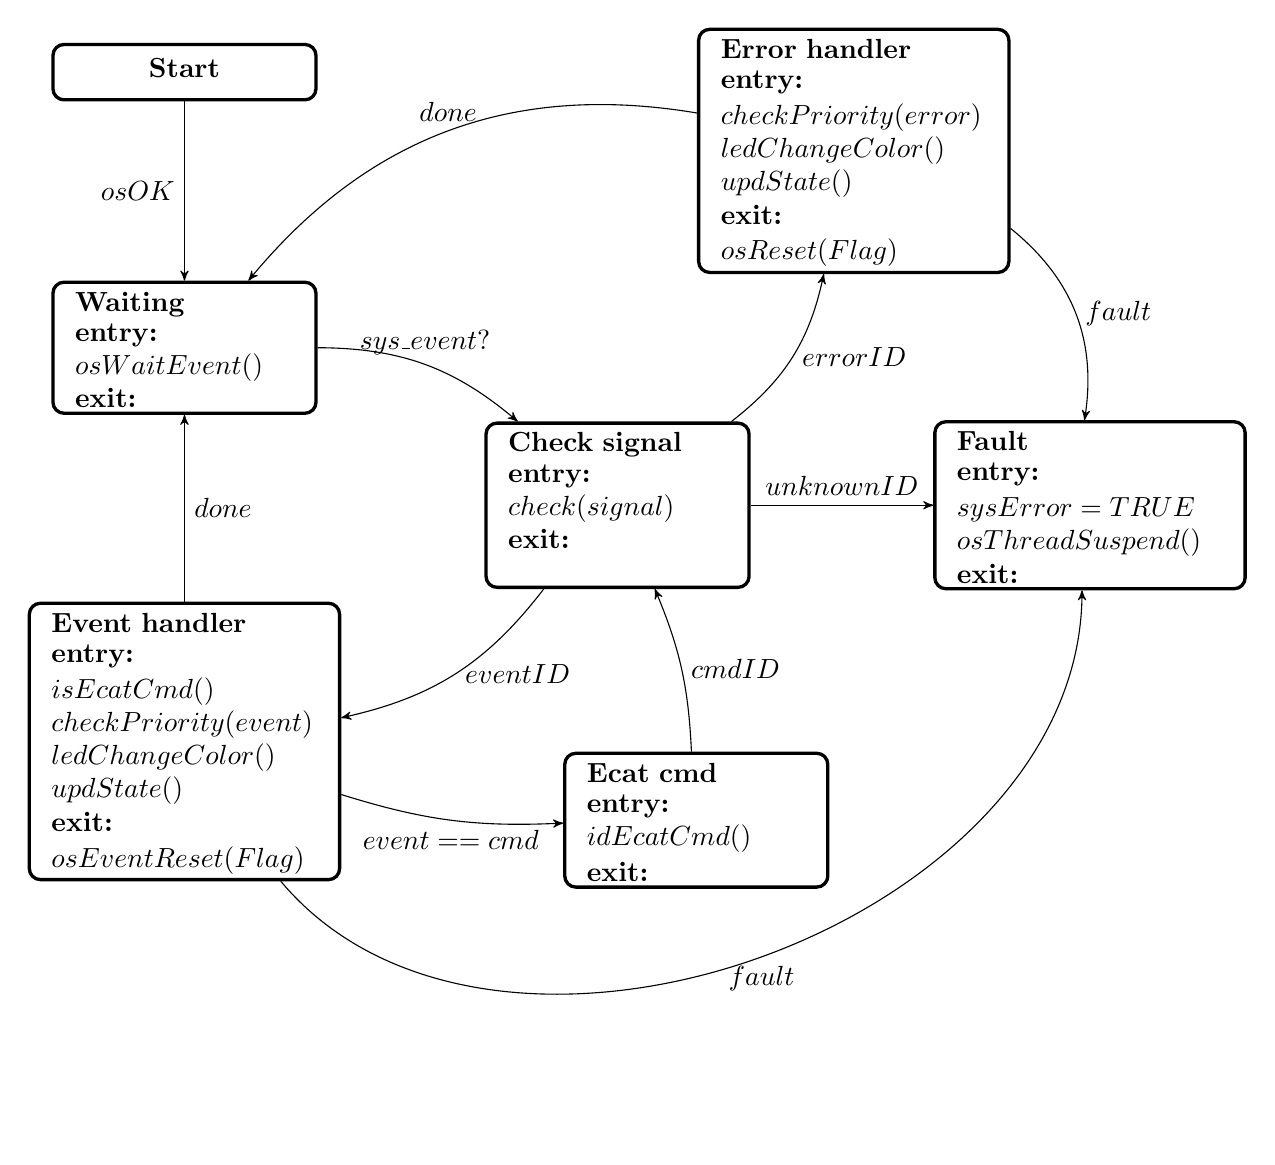
\begin{tikzpicture}[->,>=stealth']
        %   Event Handler
        % Position of Start 
        % Use previously defined 'state' as layout (see above)
        % use tabular for content to get columns/rows
        % parbox to limit width of the listing
        \node[state,
            text width=3.2cm 	
            ] (EV_START) 
        {
            \begin{tabular}{l}
            \textbf{Start}\\[.1em]
            
        \end{tabular}
        };
    
      % STATE E_WAIT
      \node[state,
      text width=3.2cm,
          below of=EV_START,
          %yshift=-2cm,
          node distance=3.5cm, 
          anchor=center ] (EV_WAIT) 
        {
          \begin{tabular}{l}
          \textbf{Waiting}\\[.1em]
          \parbox{3cm}{
              \textbf{entry:}\\
              $osWaitEvent()$\\
              \textbf{exit:}
              }
      \end{tabular}
      };
    
        % State: Check
        \node[state,    	% layout (defined above)
            text width=3.2cm, 	% max text width
            yshift=-2cm, 		% move 2cm in y
            xshift=1cm,
            right of=EV_WAIT, 	% Position is to the right of QUERY
            node distance=4.5cm, 	% distance to QUERY
            anchor=center] (EV_CHCK) 	% posistion relative to the center of the 'box'
        {%
        \begin{tabular}{l} 	% content
            \textbf{Check signal}\\[.1em]
            \parbox{2.8cm}{
                \textbf{entry:}\\
                $check(signal)$\\
                \textbf{exit:}\\
                }
        \end{tabular}
        };
    
        % STATE EV_FAULT
        \node[state,
            text width=3.8cm,
            right of=EV_CHCK,
            xshift=1.5cm,
            node distance=4.5cm,
            anchor=center] (EV_FAULT) 
        {%
        \begin{tabular}{l}
        \textbf{Fault}\\[.1em]
        \parbox{4cm}{
            \textbf{entry:}\\[.1em]
            $sysError = TRUE$\\
            $osThreadSuspend()$\\
            \textbf{exit:}
            }
        \end{tabular}
        };
    
        % STATE ERROR HANDLER
        % Use previously defined 'state' as layout (see above)
        % use tabular for content to get columns/rows
        % parbox to limit width of the listing
        \node[state,
            text width=3.8cm,
            above of = EV_CHCK,
            xshift = 3cm,
            yshift = 1cm,
            node distance = 3.5cm,
            anchor = center] (EV_HANDLER_ERROR) 
        {\begin{tabular}{l}
            \textbf{Error handler}\\[.1em]
            \parbox{4cm}{
                \textbf{entry:}\\[.1em]
                $checkPriority(error)$\\
                $ledChangeColor()$\\
                $updState()$\\
                \textbf{exit:}\\[.1em]
                $osReset(Flag)$
                } 
        \end{tabular}};
    
        % STATE EVENT HANDLER
        % Use previously defined 'state' as layout (see above)
        % use tabular for content to get columns/rows
        % parbox to limit width of the listing
        \node[state,
            text width=3.8cm,
            below of = EV_WAIT,
            %xshift = -3cm,
            yshift = -1.5cm,
            node distance = 3.5cm,
            anchor = center] (EV_HANDLER_EVENT) 
        {\begin{tabular}{l}
            \textbf{Event handler}\\[.1em]
            \parbox{4cm}{
                \textbf{entry:}\\[.1em]
                $isEcatCmd()$
                $checkPriority(event)$\\
                $ledChangeColor()$\\
                $updState()$\\
                \textbf{exit:}\\[.1em]
                $osEventReset(Flag)$
                } 
        \end{tabular}};
            
    
        %STATE ECAT CMD
        \node[state,
        text width = 3.2cm,
        below of=EV_CHCK,
        yshift= 0.5cm,
        xshift = 1cm,
        node distance=4.5cm,
        anchor=center] (EV_ECATCMD) 
        {%
        \begin{tabular}{l}
        \textbf{Ecat cmd}\\[.1em]
        \parbox{4cm}{
            \textbf{entry:}\\
            $idEcatCmd()$\\[.1em]
            \textbf{exit:}
            }
        \end{tabular}
        };
    
        % EV_START
        % EV_WAIT
        % EV_CHCK
        % EV_FAULT
        % EV_HANDLER_ERROR
        % EV_HANDLER_EVENT
        % EV_ECATCMD
        % draw the paths and and print some Text below/above the graph
        \path
            (EV_START)       edge node[anchor=center,left]{$osOK$}  (EV_WAIT) 
            (EV_WAIT) 	    edge[bend left=20]  node[anchor=north,above]{$sys\_event?$} (EV_CHCK)
            (EV_CHCK)     	edge[bend right=20] node[anchor=north,right]{$errorID$} (EV_HANDLER_ERROR)
            (EV_CHCK)       	edge  node[anchor=center,above]{$unknownID$}     (EV_FAULT)
            (EV_CHCK)       	edge[bend left=20] node[anchor=center,right]{$eventID$}   (EV_HANDLER_EVENT)
            % (E_CONNECTED)   edge            node[anchor=north,above]{$soes$}     
            %                                 node[anchor=south,below]{$timeout$}(E_FAULT)
            (EV_HANDLER_ERROR)   edge[bend right=30]  node[anchor=center,above]{$done$}   (EV_WAIT)
            (EV_HANDLER_ERROR)   edge[bend left=30]  node[anchor=center,right]{$fault$}   (EV_FAULT)
            % (E_FAULT)  	    edge            node[anchor=north,above]{$thread$} 
            %                                 node[anchor=center,below]{$removed?$}   (E_RESTART)
            (EV_HANDLER_EVENT)  	edge  node[anchor=center,right]{$done$}     (EV_WAIT)
            (EV_HANDLER_EVENT)  	edge[bend right=10] node[anchor=center,below]{$event==cmd$}(EV_ECATCMD)     
                                                        %node[anchor=center,below]{$==cmd$}
            (EV_HANDLER_EVENT)  	edge[bend right=70] node[anchor=center,below]{$fault$}     (EV_FAULT)
            (EV_ECATCMD)  	edge[bend right=10]  node[anchor=center,right]{$cmdID$}     (EV_CHCK)
            ;
    
        \end{tikzpicture}
    \caption{State machine for Event Handler functionality.}
    \label{fig:sm_event}
\end{figure}





%LED DSM
\begin{figure}[ht]
    \centering
    %Her comes the figure
    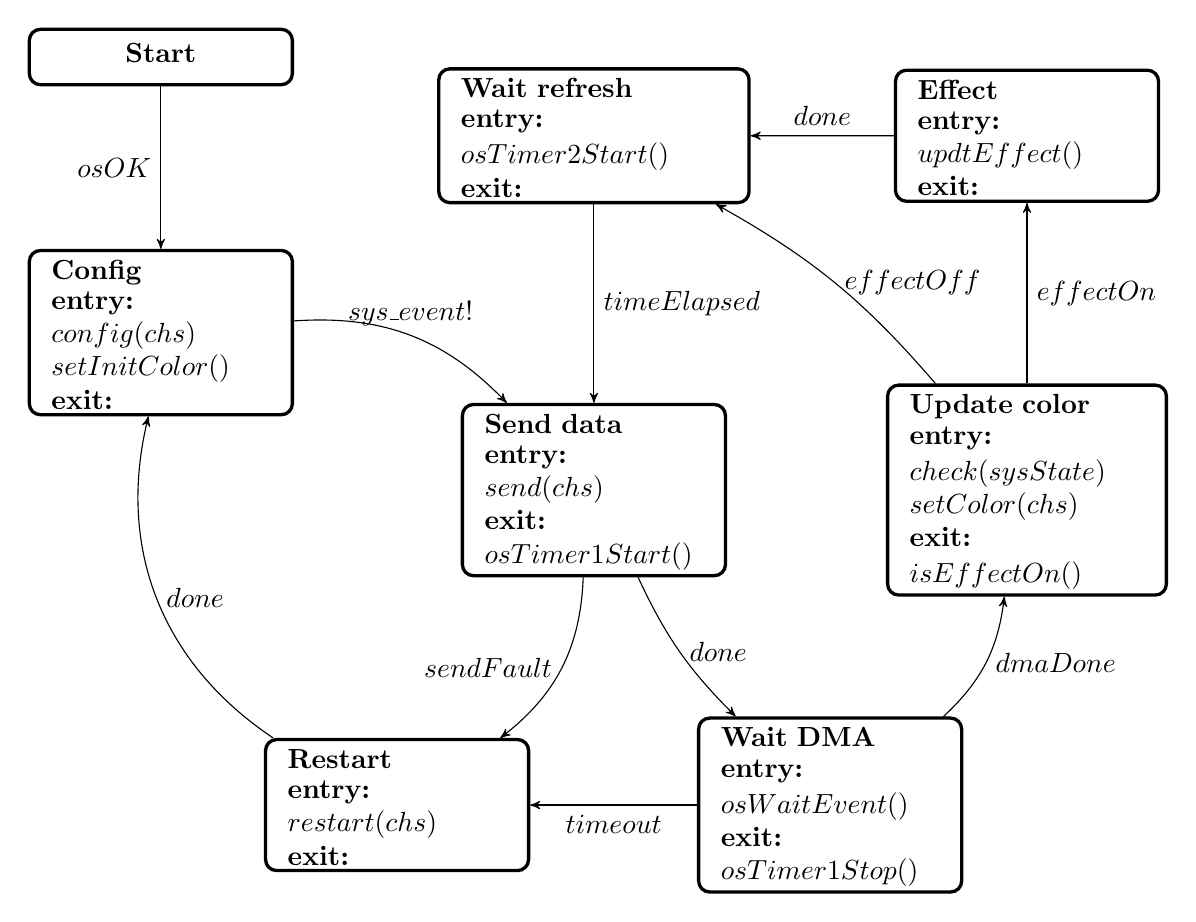
\begin{tikzpicture}[->,>=stealth']
        %   LED DSM
        % Position of Start 
        % Use previously defined 'state' as layout (see above)
        % use tabular for content to get columns/rows
        % parbox to limit width of the listing
        \node[state,
            text width=3.2cm 	
            ] (L_START) 
        {
            \begin{tabular}{l}
            \textbf{Start}\\[.1em]
            
        \end{tabular}
        };
    
      % STATE L_CONFIG
      \node[state,
      text width=3.2cm,
          below of=L_START,
          %yshift=-2cm,
          node distance=3.5cm, 
          anchor=center ] (L_CONFIG) 
        {
          \begin{tabular}{l}
          \textbf{Config}\\[.1em]
          \parbox{3cm}{
              \textbf{entry:}\\
              $config(chs)$\\
              $setInitColor()$
              \textbf{exit:}
              }
      \end{tabular}
      };
    
    
        % State: L_SEND
        \node[state,    	% layout (defined above)
            text width=3.2cm, 	% max text width
            yshift=-2cm, 		% move 2cm in y
            xshift=1cm,
            right of=L_CONFIG, 	% Position is to the right of QUERY
            node distance=4.5cm, 	% distance to QUERY
            anchor=center] (L_SEND) 	% posistion relative to the center of the 'box'
        {%
        \begin{tabular}{l} 	% content
            \textbf{Send data}\\[.1em]
            \parbox{2.8cm}{
                \textbf{entry:}\\
                $send(chs)$\\
                \textbf{exit:}\\
                $osTimer1Start()$
                }
        \end{tabular}
        };
    
        % STATE L_WAIT_REFRESH
        \node[state,
            text width=3.8cm,
            above of=L_SEND,
            %xshift=1.5cm,
            node distance=4.5cm,
            anchor=center] (L_WAIT_REFRESH) 
        {%
        \begin{tabular}{l}
        \textbf{Wait refresh}\\[.1em]
        \parbox{4cm}{
            \textbf{entry:}\\[.1em]
            $osTimer2Start()$\\
            \textbf{exit:}
            }
        \end{tabular}
        };
    
    
    
    
        % STATE L_C_UPDATE
        % Use previously defined 'state' as layout (see above)
        % use tabular for content to get columns/rows
        % parbox to limit width of the listing
        \node[state,
            text width=3.4cm,
            right of = L_SEND,
            xshift = 1cm,
            %yshift = -1.5cm,
            node distance = 4.5cm,
            anchor = center] (L_C_UPDATE) 
        {\begin{tabular}{l}
            \textbf{Update color}\\[.1em]
            \parbox{4cm}{
                \textbf{entry:}\\[.1em]
                $check(sysState)$
                $setColor(chs)$\\
                \textbf{exit:}\\[.1em]
                $isEffectOn()$
                } 
        \end{tabular}};
    
    
        % STATE 
        % Use previously defined 'state' as layout (see above)
        % use tabular for content to get columns/rows
        % parbox to limit width of the listing
        \node[state,
            text width=3.2cm,
            below of = L_C_UPDATE,
            xshift = -2.5cm,
            %yshift = -3.5cm,
            node distance = 4cm,
            anchor = center] (L_WAIT_DMA) 
        {\begin{tabular}{l}
            \textbf{Wait DMA}\\[.1em]
            \parbox{4cm}{
                \textbf{entry:}\\[.1em]
                $osWaitEvent()$\\
                \textbf{exit:}\\
                $osTimer1Stop()$
                } 
        \end{tabular}};
    
        %STATE L_EFFECT
        \node[state,
        text width = 3.2cm,
        above of=L_C_UPDATE,
        yshift= 1cm,
        %xshift = 1cm,
        node distance=3.5cm,
        anchor=center] (L_EFFECT) 
        {%
        \begin{tabular}{l}
        \textbf{Effect}\\[.1em]
        \parbox{4cm}{
            \textbf{entry:}\\
            $updtEffect()$\\
            \textbf{exit:}
            }
        \end{tabular}
        };
    
            %STATE L_RESTART
        \node[state,
        text width = 3.2cm,
        below of=L_SEND,
        %yshift= 0.5cm,
        xshift = -2.5cm,
        node distance=4cm,
        anchor=center] (L_RESTART) 
        {%
        \begin{tabular}{l}
        \textbf{Restart}\\[.1em]
        \parbox{4cm}{
            \textbf{entry:}\\
            $restart(chs)$\\
            \textbf{exit:}
            }
        \end{tabular}
        };
    
        % L_START
        % L_CONFIG
        % L_WAIT_DMA
        % L_SEND
        % L_C_UPDATE
        % L_WAIT_REFRESH
        % L_EFFECT
        % L_RESTART  
    
        % draw the paths and and print some Text below/above the graph
        \path
            (L_START)       edge node[anchor=center,left]{$osOK$}  (L_CONFIG) 
            (L_CONFIG) 	    edge[bend left=25]  node[anchor=north,above]{$sys\_event!$} (L_SEND)
            (L_SEND)     	edge[bend right=10] node[anchor=north,right]{$done$} (L_WAIT_DMA)
            (L_WAIT_DMA)       	edge[bend right=20]  node[anchor=center,right]{$dmaDone$}     (L_C_UPDATE)
            (L_WAIT_DMA)       	edge  node[anchor=center,below]{$timeout$}     (L_RESTART)
            (L_C_UPDATE)       	edge[bend right=10] node[anchor=center,right]{$effectOff$}   (L_WAIT_REFRESH)
            (L_C_UPDATE)   edge node[anchor=center,right]{$effectOn$}   (L_EFFECT)
            (L_EFFECT)   edge  node[anchor=center,above]{$done$}   (L_WAIT_REFRESH)
            % (E_FAULT)  	    edge            node[anchor=north,above]{$thread$} 
            %                                 node[anchor=center,below]{$removed?$}   (E_RESTART)
            (L_WAIT_REFRESH)  	edge  node[anchor=center,right]{$timeElapsed$}     (L_SEND)
            % (L_SEND)  	edge[bend right=10] node[anchor=center,below]{$event==cmd$}(EV_ECATCMD)     
            %                                             %node[anchor=center,below]{$==cmd$}
            (L_SEND)  	edge[bend left=25] node[anchor=center,left]{$sendFault$}     (L_RESTART)
            (L_RESTART)  	edge[bend left=35]  node[anchor=center,right]{$done$}     (L_CONFIG)
            ;
    
        \end{tikzpicture}
    \caption{State machine for LED Ring control functionality}
    \label{fig:sm_led}
\end{figure}




\begin{figure}[ht]
    \centering
    \subfigure[Synchronization state machine]{\label{subfig:ecat_sm}{
        %General state machine 80/100
        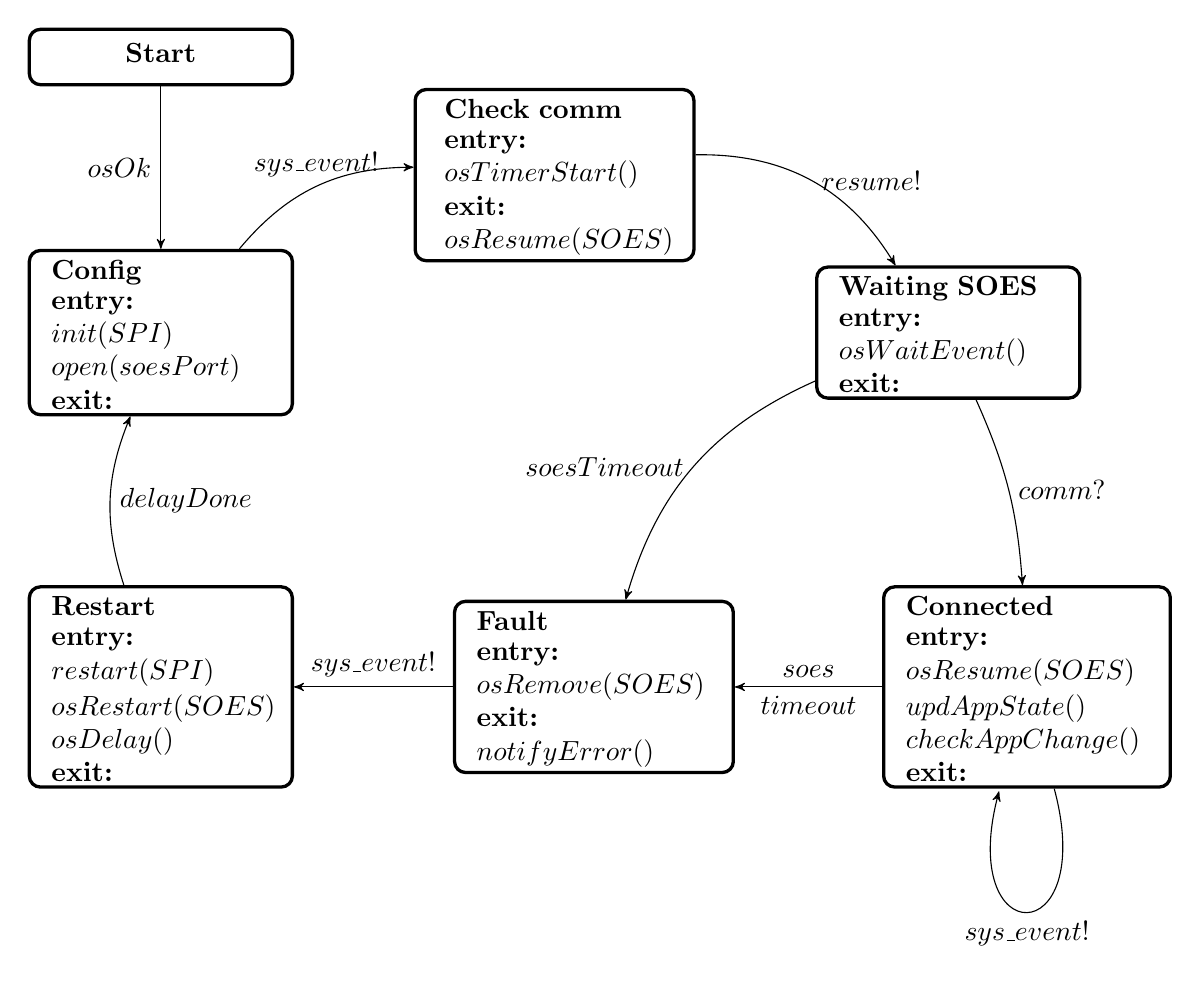
\begin{tikzpicture}[->,>=stealth']
        % Position of QUERY 
        % Use previously defined 'state' as layout (see above)
        % use tabular for content to get columns/rows
        % parbox to limit width of the listing
        \node[state,
            text width=3.2cm 	
            ] (E_CONFIG) 
        {\begin{tabular}{l}
            \textbf{Config}\\[.1em]
            \parbox{4cm}{
            \textbf{entry:}\\
            $init(SPI)$\\
            $open(soesPort)$\\
            \textbf{exit:}
            }
        \end{tabular}};
  
        % STATE START 
        % Use previously defined 'state' as layout (see above)
        % use tabular for content to get columns/rows
        % parbox to limit width of the listing
        \node[state,
            text width=3.2cm,
            above of = E_CONFIG,
            node distance = 3.5cm,
            anchor = center] (E_START) 
        {\begin{tabular}{l}
            \textbf{Start}\\[.1em]
            
        \end{tabular}};
  
  
            
        % State: ACK with different content
        \node[state,    	% layout (defined above)
            text width=3.4cm, 	% max text width
            yshift=2cm, 		% move 2cm in y
            right of=E_CONFIG, 	% Position is to the right of QUERY
            node distance=5cm, 	% distance to QUERY
            anchor=center] (E_CHCK) 	% posistion relative to the center of the 'box'
        {%
        \begin{tabular}{l} 	% content
            \textbf{Check comm}\\[.1em]
            \parbox{2.8cm}{
                \textbf{entry:}\\
                $osTimerStart()$
                \textbf{exit:}\\
                $osResume(SOES)$
                }
        \end{tabular}
        };
        
        % STATE E_WAIT
        \node[state,
        text width=3.2cm,
            %below of=ACK,
            right of=E_CHCK,
            yshift=-2cm,
            node distance=5cm, 
            anchor=center ] (E_WAIT) 
        {%
        \begin{tabular}{l}
            \textbf{Waiting SOES}\\[.1em]
            \parbox{2.8cm}{
                \textbf{entry:}\\
                $osWaitEvent()$\\
                \textbf{exit:}
                }
        \end{tabular}
        };
        
  
        
        %STATE CONNECTED
        \node[state,
        text width = 3.5cm,
        below of=E_WAIT,
        xshift= 1cm,
        node distance=4.5cm,
        anchor=center] (E_CONNECTED) 
        {%
        \begin{tabular}{l}
        \textbf{Connected}\\[.1em]
        \parbox{4cm}{
            \textbf{entry:}\\
            $osResume(SOES)$\\[.1em]
            $updAppState()$\\
            $checkAppChange()$\\
            \textbf{exit:}
            }
        \end{tabular}
        };
  
        % STATE E_FAULT
        \node[state,
            text width=3.4cm,
            left of=E_CONNECTED,
            %xshift=-2.5cm,
            node distance=5.5cm,
            anchor=center] (E_FAULT) 
        {%
        \begin{tabular}{l}
        \textbf{Fault}\\[.1em]
        \parbox{4cm}{
            \textbf{entry:}\\
            $osRemove(SOES)$\\
            \textbf{exit:}\\
            $notifyError()$
            }
        \end{tabular}
        };
  
        %STATE RESTART
        \node[state,
        text width = 3.2cm,
        left of=E_FAULT,
        node distance=5.5cm,
        %xshift = 2cm,
        anchor=center] (E_RESTART) 
        {%
        \begin{tabular}{l}
        \textbf{Restart}\\[.1em]
        \parbox{4cm}{
            \textbf{entry:}\\
            $restart(SPI)$\\[.1em]
            $osRestart(SOES)$\\
            $osDelay()$\\
            \textbf{exit:}
            }
        \end{tabular}
        };
  
        % draw the paths and and print some Text below/above the graph
        \path
            (E_START)       edge node[anchor=center,left]{$osOk$}  (E_CONFIG) 
            (E_CONFIG) 	    edge[bend left=25]  node[anchor=center,above]{$sys\_event!$} (E_CHCK)
            (E_CHCK)     	edge[bend left=30] node[anchor=north,right]{$resume!$} (E_WAIT)
            (E_WAIT)       	edge[bend left=10]  node[anchor=center,right]{$comm?$}     (E_CONNECTED)
            (E_WAIT)       	edge[bend right=25] node[anchor=center,left]{$soesTimeout$}                                         (E_FAULT)
            (E_CONNECTED)   edge            node[anchor=north,above]{$soes$}     
                                            node[anchor=south,below]{$timeout$}(E_FAULT)
            (E_CONNECTED)   edge[loop below]  node[anchor=left,below]{$sys\_event!$}                   (E_CONNECTED)
            (E_FAULT)  	    edge            node[anchor=north,above]{$sys\_event!$} (E_RESTART)
            %                                node[anchor=center,below]{$removed?$}   (E_RESTART)
            (E_RESTART)  	edge[bend left=20]  node[anchor=center,right]{$delayDone$}                                          (E_CONFIG)
            ;
  
        \end{tikzpicture}
    }}\hfill
    \subfigure[SOES application state machine]{\label{subfig:soes_sm}{
        %SOES state machine 80/100
        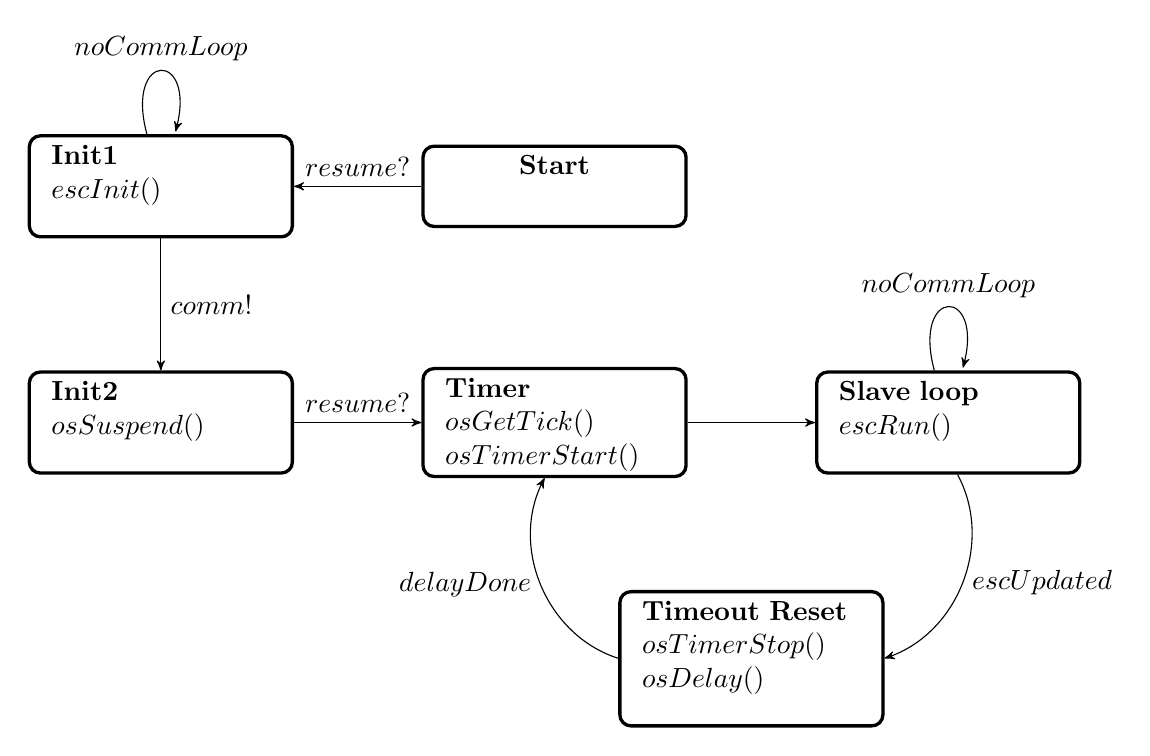
\begin{tikzpicture}[->,>=stealth']
        % STATE 1 SOES
        % Use previously defined 'state' as layout (see above)
        % use tabular for content to get columns/rows
        % parbox to limit width of the listing
        \node[state,
            text width=3.2cm 	
            ] (SOES_INIT1) 
        {\begin{tabular}{l}
            \textbf{Init1}\\[.1em]
            \parbox{4cm}{
            
            $escInit()$\\
            
            }
        \end{tabular}};
            
        % STATE SOES INIT 2
        \node[state,    	% layout (defined above)
            text width=3.2cm, 	% max text width
            %yshift=2cm, 		% move 2cm in y
            below of=SOES_INIT1, 	
            node distance=3cm, 	% 
            anchor=center] (SOES_INIT2) 	% posistion relative to the center of the 'box'
        {%
        \begin{tabular}{l} 	% content
            \textbf{Init2}\\[.1em]
            \parbox{2.8cm}{
                $osSuspend()$\\
                }
        \end{tabular}
        };
  
        % STATE 0 SOES
        % Use previously defined 'state' as layout (see above)
        % use tabular for content to get columns/rows
        % parbox to limit width of the listing
        \node[state,
            text width=3.2cm,
            right of = SOES_INIT1,
            node distance = 5cm,
            anchor = center] (SOES_INIT0) 
        {\begin{tabular}{l}
            \textbf{Start}\\[.1em]
            \parbox{4cm}{
            
            }
        \end{tabular}};
        
        % STATE SET TIMER
        \node[state,
        text width=3.2cm,
            %below of=ACK,
            right of=SOES_INIT2,
            %yshift=-2cm,
            node distance=5cm, 
            anchor=center ] (SOES_TIMER) 
        {%
        \begin{tabular}{l}
            \textbf{Timer}\\[.1em]
            \parbox{2.8cm}{
                $osGetTick()$\\
                $osTimerStart()$
                }
        \end{tabular}
        };
        
  
        
        %STATE SLAVE LOOP
        \node[state,
        text width = 3.2cm,
        right of=SOES_TIMER,
        %xshift= 2.5cm,
        node distance=5cm,
        anchor=center] (SOES_SLAVE) 
        {%
        \begin{tabular}{l}
        \textbf{Slave loop}\\[.1em]
        \parbox{4cm}{
            $escRun()$\\
            }
        \end{tabular}
        };
  
        % STATE SOES_RESET TIMEOUT
        \node[state,
            text width=3.2cm,
            below of=SOES_SLAVE,
            xshift=-2.5cm,
            node distance=3cm,
            anchor=center] (SOES_RESET) 
        {%
        \begin{tabular}{l}
        \textbf{Timeout Reset}\\[.1em]
        \parbox{4cm}{
            $osTimerStop()$\\
            $osDelay()$\\
            }
        \end{tabular}
        };
  
        
        draw the paths and and print some Text below/above the graph
        \path
        (SOES_INIT0)    edge node[anchor=center,above]{$resume?$} (SOES_INIT1) 
        (SOES_INIT1) 	edge  node[anchor=south,right]{$comm!$}  (SOES_INIT2)
        (SOES_INIT1)    edge [loop above]   node[anchor=east,above]{$noCommLoop$} (SOES_INIT1)
        (SOES_INIT2)    edge node [anchor=center,above]{$resume?$} (SOES_TIMER)                                          (SOES_TIMER)
        (SOES_TIMER)    edge                   (SOES_SLAVE)
        (SOES_SLAVE)    edge [loop above]       node[anchor=center,above]{$noCommLoop$}       (SOES_SLAVE)
        (SOES_SLAVE)    edge [bend left = 50]   node[anchor=center,right]{$escUpdated$}   (SOES_RESET)
        (SOES_RESET)    edge [bend left = 50]   node[anchor=center,left]{$delayDone$}   (SOES_TIMER)
        ;
  
        \end{tikzpicture}
    }}
    \caption{State machines for EtherCAT slave functionality.} %EtherCAT Device Protocol poster from EtherCAT resources
    \label{fig:sm_ecatsoes}
  \end{figure} 

% \begin{figure}[ht]
%     \centering
%     \subfigure[Synchronization state machine]{\label{subfig:ecat_sm}{
%         %General state machine 80/100
%         \begin{tikzpicture}[->,>=stealth']
%         % Position of QUERY 
%         % Use previously defined 'state' as layout (see above)
%         % use tabular for content to get columns/rows
%         % parbox to limit width of the listing
%         \node[state,
%             text width=3.2cm 	
%             ] (E_CONFIG) 
%         {\begin{tabular}{l}
%             \textbf{Config}\\[.1em]
%             \parbox{4cm}{
%             \textbf{entry:}\\
%             $spi\_init()$\\
%             $open\_soesPort()$\\
%             \textbf{exit:}
%             }
%         \end{tabular}};

%         % STATE START 
%         % Use previously defined 'state' as layout (see above)
%         % use tabular for content to get columns/rows
%         % parbox to limit width of the listing
%         \node[state,
%             text width=3.2cm,
%             above of = E_CONFIG,
%             node distance = 3.5cm,
%             anchor = center] (E_START) 
%         {\begin{tabular}{l}
%             \textbf{Start}\\[.1em]
            
%         \end{tabular}};


            
%         % State: ACK with different content
%         \node[state,    	% layout (defined above)
%             text width=3.2cm, 	% max text width
%             yshift=2cm, 		% move 2cm in y
%             right of=E_CONFIG, 	% Position is to the right of QUERY
%             node distance=5cm, 	% distance to QUERY
%             anchor=center] (E_CHCK) 	% posistion relative to the center of the 'box'
%         {%
%         \begin{tabular}{l} 	% content
%             \textbf{Check comm}\\[.1em]
%             \parbox{2.8cm}{
%                 \textbf{entry:}\\
%                 $timeout\_start()$
%                 \textbf{exit:}\\
%                 $resume\_SOES()$
%                 }
%         \end{tabular}
%         };
        
%         % STATE E_WAIT
%         \node[state,
%         text width=3.2cm,
%             %below of=ACK,
%             right of=E_CHCK,
%             yshift=-2cm,
%             node distance=5cm, 
%             anchor=center ] (E_WAIT) 
%         {%
%         \begin{tabular}{l}
%             \textbf{Waiting SOES}\\[.1em]
%             \parbox{2.8cm}{
%                 \textbf{entry:}\\
%                 $osWaitEvent()$\\
%                 \textbf{exit:}
%                 }
%         \end{tabular}
%         };
        

        
%         %STATE CONNECTED
%         \node[state,
%         text width = 3.2cm,
%         below of=E_WAIT,
%         xshift= 2.5cm,
%         node distance=4.5cm,
%         anchor=center] (E_CONNECTED) 
%         {%
%         \begin{tabular}{l}
%         \textbf{Connected}\\[.1em]
%         \parbox{4cm}{
%             \textbf{entry:}\\
%             $osResume(SOES)$\\[.1em]
%             $update\_state()$\\
%             \textbf{exit:}
%             }
%         \end{tabular}
%         };

%         % STATE E_FAULT
%         \node[state,
%             text width=3.2cm,
%             below of=E_WAIT,
%             xshift=-2.5cm,
%             node distance=4.5cm,
%             anchor=center] (E_FAULT) 
%         {%
%         \begin{tabular}{l}
%         \textbf{Fault}\\[.1em]
%         \parbox{4cm}{
%             \textbf{entry:}\\
%             $notify\_error()$\\
%             $osThreadRemove()$\\
%             \textbf{exit:}
%             }
%         \end{tabular}
%         };

%         %STATE RESTART
%         \node[state,
%         text width = 3.2cm,
%         left of=E_FAULT,
%         node distance=5cm,
%         %xshift = 2cm,
%         anchor=center] (E_RESTART) 
%         {%
%         \begin{tabular}{l}
%         \textbf{Restart}\\[.1em]
%         \parbox{4cm}{
%             \textbf{entry:}\\
%             $deInit_SPI()$\\[.1em]
%             $restartSOES$\\
%             $delay()$
%             }
%         \end{tabular}
%         };

%         % draw the paths and and print some Text below/above the graph
%         \path
%             (E_START)       edge node[anchor=center,left]{$os\_ready$}  (E_CONFIG) 
%             (E_CONFIG) 	    edge[bend left=20]  node[anchor=north,above]{$port\_ok$} (E_CHCK)
%             (E_CHCK)     	edge[bend left=20] node[anchor=north,right]{$Resume!$} (E_WAIT)
%             (E_WAIT)       	edge[bend left=10]  node[anchor=center,right]{$Comm?$}     (E_CONNECTED)
%             (E_WAIT)       	edge[bend right=10] node[anchor=center,left]{$soes\_timeout$}                                         (E_FAULT)
%             (E_CONNECTED)   edge            node[anchor=north,above]{$soes$}     
%                                             node[anchor=south,below]{$timeout$}(E_FAULT)
%             (E_CONNECTED)   edge[loop below]  node[anchor=center,below]{$update\_loop$}                   (E_CONNECTED)
%             (E_FAULT)  	    edge            node[anchor=north,above]{$thread$} 
%                                             node[anchor=center,below]{$removed?$}   (E_RESTART)
%             (E_RESTART)  	edge[bend left=30]  node[anchor=center,left]{$delay\_done$}                                          (E_CONFIG)
%             ;

%         \end{tikzpicture}
%     }}\hfill
%     \subfigure[SOES application state machine]{\label{subfig:soes_sm}{
%         %SOES state machine 80/100
%         \begin{tikzpicture}[->,>=stealth']
%         % STATE 1 SOES
%         % Use previously defined 'state' as layout (see above)
%         % use tabular for content to get columns/rows
%         % parbox to limit width of the listing
%         \node[state,
%             text width=3.2cm 	
%             ] (SOES_INIT1) 
%         {\begin{tabular}{l}
%             \textbf{Init1}\\[.1em]
%             \parbox{4cm}{
            
%             $lib\_init()$\\
            
%             }
%         \end{tabular}};
            
%         % STATE SOES INIT 2
%         \node[state,    	% layout (defined above)
%             text width=3.2cm, 	% max text width
%             %yshift=2cm, 		% move 2cm in y
%             below of=SOES_INIT1, 	
%             node distance=3cm, 	% 
%             anchor=center] (SOES_INIT2) 	% posistion relative to the center of the 'box'
%         {%
%         \begin{tabular}{l} 	% content
%             \textbf{Init2}\\[.1em]
%             \parbox{2.8cm}{
%                 $suspend\_thread()$\\
%                 }
%         \end{tabular}
%         };

%         % STATE 0 SOES
%         % Use previously defined 'state' as layout (see above)
%         % use tabular for content to get columns/rows
%         % parbox to limit width of the listing
%         \node[state,
%             text width=3.2cm,
%             right of = SOES_INIT1,
%             node distance = 5cm,
%             anchor = center] (SOES_INIT0) 
%         {\begin{tabular}{l}
%             \textbf{Start}\\[.1em]
%             \parbox{4cm}{
            
%             }
%         \end{tabular}};
        
%         % STATE SET TIMER
%         \node[state,
%         text width=3.2cm,
%             %below of=ACK,
%             right of=SOES_INIT2,
%             %yshift=-2cm,
%             node distance=5cm, 
%             anchor=center ] (SOES_TIMER) 
%         {%
%         \begin{tabular}{l}
%             \textbf{Timer}\\[.1em]
%             \parbox{2.8cm}{
%                 $osGetTick()$\\
%                 $osStartTimeout()$
%                 }
%         \end{tabular}
%         };
        

        
%         %STATE SLAVE LOOP
%         \node[state,
%         text width = 3.2cm,
%         right of=SOES_TIMER,
%         %xshift= 2.5cm,
%         node distance=5cm,
%         anchor=center] (SOES_SLAVE) 
%         {%
%         \begin{tabular}{l}
%         \textbf{Slave loop}\\[.1em]
%         \parbox{4cm}{
%             $eca\_slv()$\\
%             }
%         \end{tabular}
%         };

%         % STATE SOES_RESET TIMEOUT
%         \node[state,
%             text width=3.2cm,
%             below of=SOES_SLAVE,
%             xshift=-2.5cm,
%             node distance=3cm,
%             anchor=center] (SOES_RESET) 
%         {%
%         \begin{tabular}{l}
%         \textbf{Timeout Reset}\\[.1em]
%         \parbox{4cm}{
%             $reset\_Timeout()$\\
%             $osDelay()$\\
%             }
%         \end{tabular}
%         };

        
%         draw the paths and and print some Text below/above the graph
%         \path
%         (SOES_INIT0)    edge node[anchor=center,above]{$Resume?$} (SOES_INIT1) 
%         (SOES_INIT1) 	edge  node[anchor=south,right]{$Comm!$}  (SOES_INIT2)
%         (SOES_INIT1)    edge [loop above]   node[anchor=east,above]{$no\_comm\_loop$} (SOES_INIT1)
%         (SOES_INIT2)    edge [loop below]   node[anchor=south,below]{$no\_eventFlag$} (SOES_INIT2)
%         (SOES_INIT2)    edge node [anchor=center,above]{$Resume?$} (SOES_TIMER)                                          (SOES_TIMER)
%         (SOES_TIMER)    edge                   (SOES_SLAVE)
%         (SOES_SLAVE)    edge [loop above]       node[anchor=center,above]{$no\_comm\_loop$}       (SOES_SLAVE)
%         (SOES_SLAVE)    edge [bend left = 50]   node[anchor=center,right]{$esc\_updated$}   (SOES_RESET)
%         (SOES_RESET)    edge [bend left = 50]   node[anchor=center,left]{$delay\_done$}   (SOES_TIMER)
%         ;

%         \end{tikzpicture}
%     }}
%     \caption{State machines for EtherCAT slave functionality} %EtherCAT Device Protocol poster from EtherCAT resources
%     \label{fig:syncmodes}
% \end{figure} 

% \begin{figure}[ht]
%     \centering
%     %Her comes the figure
%     \caption{This is a figure}
%     \label{fig:this_is_a_label}
% \end{figure}

% The End
\end{document}


